%
%  Introduction
%
%-- Chapter Title
\chapter{Introduction}
\noindent
The Immersed Boundary (IB) Method, introduced by Peskin~\cite{Peskin77}, offers a flexible approach  for the simulation of flow-structure interaction. It combines a Lagrangian representation of 
the immersed structures with  an Eulerian flow description.  The Lagrangian representation of the immersed boundaries endows the method with a versatile structure-building capability while the  Eulerian flow description permits  the use of fast flow solvers. The connection of the two representations is done seamlessly through {\em spreading} (of interfacial forces) and {\em interpolation} (of velocity at the immersed boundary) steps via mollified delta functions.

The flexibility of the Immersed Boundary Method has lead to its adoption for the computational simulation of a staggering number of diverse applications. A great deal of work has been done utilizing the method to simulate the cardiac fluid dynamics of blood flow through hearts
\cite{mcqueen2002heart,McQueenPeskin2000,McQueen-Peskin89,mcqueen1997shared}. Indeed, one of the original applications by Peskin himself was to study flow past artificial heart valves \cite{peskin1972flow}. The method has found use on smaller length scale applications as well, such as modeling the unsteady flows involved in insect flight \cite{miller2004vortices,miller2009flexible} and investigating air flow inside the cochlea \cite{beyer1992computational}. The method has found use modeling biological cells, including aggregates of red blood cells \cite{liu2006rheology}. Additional work is being carried out to extend the method to smaller regimes where Brownian motion plays an important role \cite{atzberger2007stochastic} in the fluid dynamics. The method is easily wed to models of complex fluids; for example, to model the peristalsis of polymeric fluids \cite{teran2008peristaltic,chrispell2010peristaltic}, as well as to investigate the effects that viscoelastic fluid responses can have on the speed of microswimmers~\cite{teran2010viscoelastic}.
  
The immersed structures used in these and other applications often have very stiff components and as a consequence strong  {\em tangential} forces are generated,  which in turn   induce severe time-step restrictions for explicit discretization~\cite{SW95,SW99}.  Fully implicit discretizations remove this  hindering constraint but are seemingly impractical due to their elevated cost~\cite{TP92, MP93}.

Progress has been made eliminating stiffness for the case of simple periodic interfaces, as in the work of Hou and Shi~\cite{HS2008b,HS2008a}.
For the more general case involving non-periodic interfaces in 2D and 3D, some encouraging results have been obtained using Krylov subspace methods to solve suitable semi-implicit discretizations~\cite{MP93,MP2008,le2009implicit}. Krylov methods are often ineffectual when the relevant	 linear or linearized system is non-definite, which is a common occurrence for Immersed Boundary applications. Krylov methods also often suffer from increased costs as the resolution of the simulation increases, requiring more iterations to achieve the same degree of convergence.

This work seeks to eliminate stiffness in the fully general case, where immersed structures need not be periodic or even continuous and can include cross links, tethers, and other important structure building components. In addition to differences in geometry, immersed structures also differ in the force they exert on the surrounding fluid. This force can be an arbitrary function of the 	structural configuration and time, and in general can make the task of removing stiffness arbitrarily difficult. Our methods developed here do not apply to all cases of force functions, but do apply to a wide range of cases, including important linear and non-linear cases, as well as cases where the Jacobian of the linearized force is both definite and non-definite. Additionally, we demonstrate that our iterative methods scale very well for high resolutions.

The methods developed here are iterative methods for solving robust, semi-implicit discretizations of the Immersed Boundary Method. Such discretizations are well known. Indeed, one such discretization was introduced by Peskin~\cite{Peskin77} in the late 70's, in which
the spreading and interpolation operators are lagged, i.e. evaluated at the current interfacial configuration rather than at the future one. Newren, Fogelson, Guy, and Kirby
proved that this scheme, in its first order or second order Crank-Nicolson form, is unconditionally stable when inertia is neglected and the interfacial  force is linear and self-adjoint~\cite{NFGK2007}. Numerical experiments in~\cite{NFGK2007}, as well as our own extensive experiments, suggest the robustness of this discretization extends to the inertial case with nonlinear interfacial force.

This semi-implicit discretization leads to a system of equations, generally nonlinear,  for the interface configuration at the future timestep. Solving this system is non-trivial and has been prohibitively expensive with previous methods. The heart of this work is developing fast methods for solving the implicit system, allowing for the efficient removal of stiffness from the IB Method.

There are two interrelated problems for removing robustly and efficiently the numerical stiffness of the IB Method:
\begin{enumerate}
\item The design of efficient solvers for the (nonlinear) system of the interface configuration.
%\item The fast evaluation of key computations used by the implicit solvers.
\item The fast evaluation of flow-mediated  interactions between immersed boundary points (flow-structure interactions).
\end{enumerate}

In this work we will attack both problems. We will focus on Krylov solvers and Multigrid methods for our implicit solvers, as well as develop a novel implicit solver for a difficult case when the fiber force is non-linear with non-definite Jacobian. The heart of this work, however, lies in the acceleration of key computations needed for these implicit solvers.

The predominant computational cost incurred by our solvers is the calculation of flow-mediated interactions between immersed boundary points. We will encapsulate this calculation in an operator which we refer to as the {\em flow-structure operator}. Accelerating the computation of this operator's output is a key component of our strategy.

In Chapter~\ref{part:Matrix}, we develop an approximate matrix representation of the flow-structure operator, as well as the entire implicit system. In many cases this representation allows for large acceleration of the implicit solvers. In addition, the matrix representation allows for the easy implementation of multigrid solvers. We provide both analytic and numerical evidence that the approximations employed do not degrade the overall accuracy of the IB Method.

In Chapter~\ref{part:Treecode} we
show that the flow-structure operator can be seen as a {\em multipole summation} with a suitable choice of potential. Using the Singular Value Decomposition and a new, efficient,  iterative algorithm we compute $L^2$-optimal far field expansions of this potential to be used in an effective treecode strategy.
 The treecode method is in some sense an extension of the matrix method, and allows for even greater acceleration. Indeed, we will see that in some cases the acceleration is so great that sophisticated solvers such as multigrid can be replaced by much simpler Krylov methods.


\chapter{The Immersed Boundary Method}
\label{part:IB}
\noindent
In the following sections we will overview the continuous equations describing the IB Method, as well as one of the most popular explicit discretizations used in numerical simulations, known as the Forward Euler/Backward Euler Method (FE/BE). In Section~\ref{Sec:Stiffness} we will then discuss the problem of stiffness.

\section{The continuous equations}
\label{Sec:Continuous}
We review the IB Method in its simplest form. We consider an incompressible, Newtonian fluid occupying a domain $\Omega \subset \mathbb{R}^2$ or $\Omega \subset \mathbb{R}^3$. Inside this domain
we assume that there is an immersed, neutrally buoyant, elastic structure. This structure may be a 1D filament or a 2D surface, but may also be a more complex,  dense 3D mesh, or some combination of all these elements. The structure need not be closed or even continuous. We refer to the set of points comprising the structure as $\Gamma$. We further assume there is some parametrization of $\Gamma$, given over a parameter space $B$. The configuration of $\Gamma$ at time $t$ is then provided in the Lagrangian form $\B{X}(s,t)$, where $s \in B$ is a Lagrangian parameter. The fluid and immersed structure form a coupled system evolving according to:
\begin{align}
\rho \left(\frac{\partial \B{u}}{\partial t} + \B{u}\cdot\nabla\B{u} \right) &= -\nabla p + \mu\nabla^2 \B{u} + \B{f}, \label{meq:momentum}\\ 
\nabla \cdot \B{u} &= 0, \label{meq:incompressibility}\\
\frac{\partial \B{X}}{\partial t}  &= \B{u}(\B{X},t), \label{meq:noslip}
\end{align}
where $\rho$ and $\mu$ are the fluid density and fluid viscosity, respectively (both assumed to be constant). Here $\B{u}(\B{x},t)$ and $p(\B{x},t)$ are the velocity field and the pressure, respectively, described in terms of the Eulerian, Cartesian coordinate $\B{x}$. The term $\B{f}$ represents the singularly supported tension force of the immersed structure acting onto the fluid. The system (\ref{meq:momentum})-(\ref{meq:noslip}) is supplemented with initial and boundary conditions. Throughout this work, we consider only periodic boundary conditions. Typically we will take $\Omega = [0,1]^2$ or $\Omega = [0,1]^3$.

The crux of the IB Method and much of its versatility is the seamless connection of the Lagrangian representation of the immersed structure with the Eulerian representation of the flow. This is achieved via the identities:
\begin{align}
\frac{\partial \B{X}}{\partial t}  &= \int_{\Omega} \B{u}(\B{x},t)\delta(\B{x}-\B{X}(s,t)) d \B{x}, \label{meq:cont_interp} \\
\B{f}(\B{x},t) &= \int_{B} \B{F}(s,t)\delta(\B{x}-\B{X}(s,t)) ds
\label{meq:cont_spread},
\end{align}
where $\delta$ denotes the (two or three-dimensional) Dirac delta distribution. In (\ref{meq:cont_spread}), $\B{F}$
represents the elastic force density of $\Gamma$ and is described in Lagrangian coordinates. Typically,   the fiber force at time $t$, $\B{F}(\cdot,t)$, is given as a function of $\B{X}(\cdot,t)$, the configuration of our immersed structure at time $t$. We denote this as
\begin{equation}
\B{F} = \C{A}(\B{X}),
\end{equation}
for some potentially nonlinear operator $\C{A}$.

The IB Method is thus a coupled system. The underlying fluid and its associated velocity field $\B{u}$ dictate the motion of the immersed structure $\B{X}$. The configuration of $\B{X}$, in turn, produces a force distribution $\C{A}(\B{X})$ which acts on the fluid.


\section{The Forward Euler/Backward Euler explicit discretization}
\label{Sec:FEBE}
One of the most commonly used schemes with an explicit treatment of the immersed boundary is the 
so-called Forward Euler/Backward Euler (FE/BE)~\cite{SW99} in which the tension force is explicit (Forward Euler) and the 
viscous term is implicit (Backward Euler). We present the FE/BE method in this section.

We start by discretizing $\Omega$ as a uniform $N\times N$ or $N\times N\times N$ Cartesian grid $\C{G}_\Omega$ with grid size $h=1/N$. We represent our structure $\Gamma$ as a collection of $N_B$ points and define $h_B=1/N_B$. Note that different conventions may be used to discretize the Lagrangian parameter space $B$ when $\Gamma$ is not one-dimensional. We call our discretization $\C{G}_B$ and take it to be a one dimensional index space, so that the discretized structure $\B{X}$ may be considered as an array of $N_B$ vectors, $\{\B{X}_i\}_{i=1}^{N_B}$. 

A common discretization used for the continuous equations (\ref{meq:momentum})-(\ref{meq:noslip}) is the Forward Euler/Backward Euler discretization, written as
\begin{align}
\rho\left(\frac{\B{u}^{n+1}-\B{u}^n}{\Delta t} + \B{u}^n\cdot\B{D}_h\B{u}^n\right) &= -\B{D}_h p^{n+1}+ \mu L_h \B{u}^{n+1} + \C{S}_n\C{A}_{h_B}(\B{X}^{n}), \label{meq:FEBE_moment} \\
\B{D}_h \cdot \B{u}^{n+1} &= 0, \label{meq:FEBE_divergence} \\
\frac{\B{X}^{n+1}-\B{X}^n}{\Delta t} &= \C{S}^*_n\B{u}^{n+1}, \label{meq:FEBE_Xt}
\end{align}
where a superscript $n$ denotes a numerical approximation taken at the time $n \Delta t$ and $\Delta t$ is the timestep. We use standard,  second order finite differences for the spatial derivatives. The spatial operators $\B{D}_h$ and $L_h$ are the standard,  second order approximations to the gradient and the Laplacian, respectively, and $\C{A}_{h_B}$ is a suitable discrete version of $\C{A}$.

$\C{S}_n$ and $ \C{S}^*_n$ are the  {\em lagged} spreading and interpolation operators, respectively. In 2D they are given by
\begin{align}
(\C{S}_n G) (\B{x})&= \sum_{s \in \C{G}_B }G(s) \delta_h(\B{x}-\B{X}^n(s))h_B,
\label{meq:S} \\
(\C{S}^*_n w)(s) &= \sum_{ \B{x} \in \C{G}_\Omega} w(\B{x})\delta_h(\B{x}-\B{X}^n(s))h^2,
\label{meq:S*}
\end{align}
where $\delta_h(\B{x}) \equiv d_h(\B{x}_0)d_h(\B{x}_1)$ and $d_h$ is an approximation of the one-dimensional Dirac delta distribution. In the 3D case we replace $h^2$ in (\ref{meq:S*}) with $h^3$ and take $\delta_h(\B{x}) \equiv d_h(\B{x}_0)d_h(\B{x}_1)d_h(\B{x}_2)$.

These operators are called lagged because the interface configuration $\B{X}^n$ is used 
instead of the future configuration $\B{X}^{n+1}$. 

There is flexibility in the choice of $d_h$ but for concreteness in the presentation we choose Peskin's 
delta~\cite{Peskin77}:
\begin{equation}
d_h(r) = \begin{cases}
\frac{1}{4h}\left( 1+\cos(\frac{\pi r}{2h})\right)& \textrm{if } |r|\leq 2h, \\
0& \textrm{otherwise}.
\end{cases}
\end{equation}

We note that while the continuous equations (\ref{meq:momentum})-(\ref{meq:noslip}) present an instantaneous coupling between $\B{u}$ and $\B{X}$, the FE/BE method decouples this system into a tick-tock evolution. Holding $\B{X}^n$ fixed we evolve the fluid to its next configuration $\B{u}^{n+1}$ by solving (\ref{meq:FEBE_moment})-(\ref{meq:FEBE_divergence}). We then hold $\B{u}^{n+1}$ fixed and calculate the updated fiber configuration $\B{X}^{n+1}$ via (\ref{meq:FEBE_Xt}). This allows us to perform FE/BE timesteps without solving any system of equations relating the interdependencies of $\B{u}$ and $\B{X}$.


\section{Stiffness}
\label{Sec:Stiffness}

The simplicity of the FE/BE method presented in the previous section has spurred its use in many IB applications. Unfortunately, while flexible enough to handle most IB applications, the method suffers from a severe timestep restriction when the immersed structure has high stiffness. Typically the timestep restraint is of the form $\Delta t = Ch\sigma^{-1/2}$, for some constant $C$ dependent on the particular problem and where $\sigma$ is a stiffness constant associated with the immersed structure which can be very large, $O(10^7)$ or more.

For a concrete example we consider the case of tether points. Tether points are fixed locations in the fluid domain to which fiber points are attracted via a Hookean spring. Each fiber point $\B{X}_i$ is associated with a tether point $\B{T}_i$ and the fiber force is then given by $\C{A}_{h_B}\B{X} = \sigma(\B{T}-\B{X})$. We consider the specific geometry of an square plate sitting in a 3D fluid with an induced flow, as described in Subsection~\ref{sub:plate}. For explicit FE/BE simulations we determine what the timestep restrictions are (shown in Table~\ref{table:ExplicitTimestep_Plate_Again}), and, moreover, what are the total computational costs for the simulation in units of CPU time (shown in Table~\ref{table:ExplicitSimulationTime_Plate}). The total simulation time is set at $T=0.25$, which is roughly the time it takes for a fluid particle in the induced flow to traverse the fluid domain $\Omega=[0,1]^3$ twice.

Increasing either $N$ or $\sigma$ leads to steep timestep restrictions and large total CPU times, on the order of months. Such restrictions are typical for many IB applications. The exorbitant costs have relegated such simulations to large computers clusters, or have prevented the simulations from being pursued altogether. The intent of this work is to remove these large computational costs, opening the possibility for preforming simulations in smaller, more agile environments, as well as opening up the possibility of simulations previously too expensive to carry out at all.

\begin{table}
\caption{ $\Delta t$ in the explicit simulations of the immersed plate for various values of $N$ and $\sigma$. $\Delta t$ is approximately the largest {\em stable} timestep, given by the formula $\Delta t =10h\sigma^{-1/2}$.}
\label{table:ExplicitTimestep_Plate_Again}
\begin{center}

\begin{tabular}{c c c c c c}
  &  $\sigma=10^7$ & $\sigma=10^8$ & $\sigma=10^9$ & $\sigma=10^{10}$ & $\sigma=10^{11}$ \\
\cline{2-6}
\multicolumn{1}{c|}{$N=32$} & \TableTopSpace
3.125\e{-5} & 9.882\e{-6} & 3.125\e{-6} & 9.882\e{-7} & 3.125\e{-7} \\
\multicolumn{1}{c|}{$N=64$}  & \TableTopSpace
1.563\e{-5} & 4.941\e{-6} & 1.563\e{-6} & 4.941\e{-7} & 1.563\e{-7} \\
\multicolumn{1}{c|}{$N=128$} & \TableTopSpace
7.813\e{-6} & 2.471\e{-6} & 7.813\e{-7} & 2.471\e{-7} & 7.813\e{-8} \\
%\cline{2-6}
\end{tabular}

\end{center}
\end{table}



\begin{table}
\caption{Total CPU time in hours for the explicit simulations of the immersed plate, with varying values of $\sigma$ and N. $^*$ denotes an extrapolated value.}
\label{table:ExplicitSimulationTime_Plate}
\begin{center}

\begin{tabular}{c c c c c c}
  &  $\sigma=10^7$ & $\sigma=10^8$ & $\sigma=10^9$ & $\sigma=10^{10}$ & $\sigma=10^{11}$ \\
\cline{2-6}
\multicolumn{1}{c|}{$N=32$} & \TableTopSpace
0.214 & 0.675 & 2.146 & 6.806 & 21.296 \\
\multicolumn{1}{c|}{$N=64$}  & \TableTopSpace
4.072 & 12.906 & 40.813$^*$ & 129.063$^*$ & 408.133$^*$ \\
\multicolumn{1}{c|}{$N=128$} & \TableTopSpace
64.779$^*$ & 204.8481$^*$ & 647.787$^*$ & 2048.481$^*$ & 6477.867$^*$ \\
%\cline{2-6}
\end{tabular}
   
\end{center}
\end{table}

\chapter{The Semi-Implicit Discretization}
\label{part:Implicit}
\noindent
We present now the implicit discretization used in this work. In Section~\ref{Sec:LagrangianSystem} we will then rearrange the resulting implicit system so that it is written in terms of the Lagrangian coordinate alone. 

\section{The semi-implicit discretization}
We employ a implicit discretization very similar to the FE/BE, taking the following form
\begin{align}
\rho\left(\frac{\B{u}^{n+1}-\B{u}^n}{\Delta t} + \B{u}^n\cdot\B{D}_h\B{u}^n\right) &= -\B{D}_h p^{n+1}+ \mu L_h \B{u}^{n+1} + \C{S}_n\C{A}_{h_B}(\B{X}^{n+1}), \label{meq:dmoment} \\
\B{D}_h \cdot \B{u}^{n+1} &= 0, \label{meq:ddivergence} \\
\frac{\B{X}^{n+1}-\B{X}^n}{\Delta t} &= \C{S}^*_n\B{u}^{n+1}. \label{meq:Xt}
\end{align}
Indeed, this discretization differs from the FE/BE discretization in only a single place, replacing the occurrence of $\B{X}^n$ in (\ref{meq:FEBE_moment}) with the future configuration $\B{X}^{n+1}$ in (\ref{meq:dmoment}).

Importantly, $\C{S}_n$ and $ \C{S}^*_n$ are the {\em lagged} spreading and interpolation operators, respectively. By lagged we mean that the location of the spreading and interpolation is determined by the old fiber configuration $\B{X}^n$. This choice makes $\C{S}_n$ and $ \C{S}^*_n$ linear operators. We stress that this linearity is critical to the numerical efficiency of our algorithm.

Newren, Fogelson, Guy, and Kirby proved that this scheme, among a family of other similar semi-implicit schemes, is unconditionally stable when inertia is neglected and the interfacial  force is linear and self-adjoint~\cite{NFGK2007}. Numerical experiments in~\cite{NFGK2007}, as well as our own extensive experiments, suggest the robustness of this discretization extends to the inertial case with nonlinear interfacial force.

The use of lagged spreading and interpolation operators in a semi-implicit scheme was originally proposed by Peskin~\cite{Peskin77} in the late 70's. However, it was not known that this scheme was stable until 2007 with the work of Newren, {\em et al.}
%Indeed, it was thought that such a scheme could not be stable.

The thrust of the present work is to find efficient and robust methods for solving the specific system of equations (\ref{meq:dmoment})-(\ref{meq:Xt}). We note, however, that the methods developed here can be easily applied to many other semi-implicit schemes in the family of schemes proved stable by Newren et al. in~\cite{NFGK2007}. In particular, there is no difficulty in adapting our methods to handle the Crank-Nicolson discretization
\begin{align}
\rho\left(\frac{\B{u}^{n+1}-\B{u}^n}{\Delta t} + \B{u}^n\cdot\B{D}_h\B{u}^n\right) &= -\B{D}_h p^{n+1}+ \mu L_h \B{u}^{n+1} + \C{S}_n\C{A}_{h_B}(\frac{1}{2}(\B{X}^n+\B{X}^{n+1})), \label{meq:cr_dmoment} \\
\B{D}_h \cdot \B{u}^{n+1} &= 0, \label{meq:cr_ddivergence} \\
\frac{\B{X}^{n+1}-\B{X}^n}{\Delta t} &= \C{S}^*_n(\frac{1}{2}(\B{u}^n+\B{u}^{n+1})). \label{meq:cr_Xt}
\end{align}
\Comment{
If we instead make use of non-lagged spreading and interpolation operators ($\C{S}_{n+1}$ and $\C{S}^*_{n+1}$), then our methodology can be used inside of a larger iterative method. Here we fix a guess $\B{X}^{n+1,k}$ for $\B{X}^{n+1}$ and then use $\B{X}^{n+1,k}$ as the configuration in $\C{S}$ and $\C{S}^*$. We can then solve the system of equations for $\B{X}^{n+1}$. We may then repeat the process, taking our result to be $\B{X}^{n+1,k+1}$ and again solving for $\B{X}^{n+1}$. We have observed good convergence for this iterative method.
}

\section{The Lagrangian system}
\label{Sec:LagrangianSystem}
The discretization (\ref{meq:dmoment})-(\ref{meq:Xt}) presents a formidable implicit system to solve. Before outlining a method of solution,  we seek a simpler representation. In particular (\ref{meq:dmoment})-(\ref{meq:Xt}) is a system of both $\B{X}^{n+1}$ and $\B{u}^{n+1}$, defined on an Eulerian and Lagrangian grid respectively. It would be convenient if we could eliminate one of these variables and work on a single grid. In this section we provide a simplified form for (\ref{meq:dmoment})-(\ref{meq:Xt}) by eliminating the occurrence of $\B{u}^{n+1}$.

Let us rewrite (\ref{meq:dmoment}) as
\begin{equation}
\B{u}^{n+1}=-\frac{\Delta t}{\rho} \B{D}_h p^{n+1} + \nu\Delta t L_h \B{u}^{n+1} + \B{a}^{n+1},
\label{meq:upa}
\end{equation}
where $\nu=\mu/\rho$ and
\begin{equation}
\B{a}^{n+1}= \frac{\Delta t}{\rho}\, \C{S}_n\C{A}_{h_B}(\B{X}^{n+1})+\B{u}^n-\Delta t \, \, \B{u}^n \cdot \nabla_h \B{u}^n. \label{meq:a}
\end{equation}
We can eliminate the pressure term in (\ref{meq:upa}) using (\ref{meq:ddivergence}), by introducing a discrete projection
$P_h$ defined as 
\begin{equation}
\B{v} = P_h \B{v} + \B{D}_h \phi_v, \qquad \B{D}_h \cdot P_h \B{v} =0, \qquad P_h \B{D}_h \phi_v=0,
\end{equation}
for any smooth vector field $\B{v}$ defined on the grid $\C{G}_{\Omega}$. Applying $P_h$ to (\ref{meq:upa}), using  (\ref{meq:ddivergence}),  and the fact that for periodic boundary conditions $L_h$ and $P_h$ commute we get
\begin{equation}
\B{u}^{n+1}= \nu\Delta t L_h \B{u}^{n+1} + P_h \B{a}^{n+1},
\end{equation}
that is
\begin{equation}
\B{u}^{n+1} = (I -\nu\Delta t L_h)^{-1}  P_h \B{a}^{n+1}.
\end{equation}
Let us denote
\begin{equation}
\C{L}_h = (I -\nu\Delta t L_h)^{-1}  P_h. \label{meq:L_h}
\end{equation}
We refer to $\C{L}_h$ as the
%\textit{fluid solver}.
\textit{flow-structure operator}.
Note that with periodic boundary conditions and a standard second order finite difference approximation for the spatial derivatives,
  $I -\nu\Delta t L_h$ is symmetric and positive definite and as a result so is its inverse. 
  On the other hand, $P_h$ is also symmetric and, being 
  a projection, it is positive semi-definite. Moreover, $P_h$ and $(I -\nu\Delta t L_h)^{-1}$ commute 
  as can be shown using the discrete Fourier transform. Consequently, these two symmetric operators can be diagonalized by the same orthogonal matrix and thus the product, $\C{L}_h $, is positive semi-definite. 

For calculations of the form $\C{L}(\B{f})$ we rely on an FFT based method, although any suitable method could be employed.
Using $\C{L}_h$,  the semi-implicit method  (\ref{meq:dmoment})-(\ref{meq:Xt})  can be expressed as
\begin{align}
\B{u}^{n+1} &= \C{L}_h \B{a}^{n+1}, \label{meq:uL} \\
\B{X}^{n+1}&=\B{X}^n +\Delta t\C{S}^*_n\B{u}^{n+1}, \label{meq:Xu}
\end{align}
where $ \B{a}^{n+1}$ is given by (\ref{meq:a}). Eliminating $\B{u}^{n+1}$ in (\ref{meq:Xu}) we obtain  a system of equations for the immersed boundary configuration $\B{X}^{n+1}$:
\begin{equation}
\B{X}^{n+1} = \C{M}_n\C{A}_{h_B} (\B{X}^{n+1}) + \B{b}^n, \label{meq:Xnl}
\end{equation}
where 
\begin{equation}
 \C{M}_n =  \alpha \,  \C{S}^*_n \C{L}_h \C{S}_n,
\label{meq:M}
\end{equation}
with
\begin{equation}
\alpha = \frac{(\Delta t)^2}{\rho}
\end{equation}
and 
\begin{equation}
 \B{b}^n = \B{X}^n + \Delta t \C{S}^*_n \C{L}_h [\B{u}^n-\Delta t \B{u}^n \cdot
 \nabla_h \B{u}^n]. \label{meq:bn}
\end{equation}
We have thus reduced (\ref{meq:dmoment})-(\ref{meq:Xt}) to a single system of  equations involving only the unknown $\B{X}^{n+1}$. After solving this system we can obtain $\B{u}^{n+1}$ via (\ref{meq:uL}). We call the linear operator $\C{M}_n$ the {\em flow-structure operator}.

Assuming we can solve (\ref{meq:Xnl}) for $\B{X}^{n+1}$ we can then calculate $\B{u}^{n+1}$ via (\ref{meq:uL}).


Note that we could just as easily eliminate $\B{X}^{n+1}$ and obtain a system involving only the unknown $\B{u}^{n+1}$, but there are two compelling reasons to prefer a system in terms of $\B{X}^{n+1}$. First, typically $N_B=|C{G}_B|$ is much smaller than $|\C{G}_\Omega|$, the number of Eulerian grid points, which is $O(N^2)$ in 2D and $O(N^3)$ in 3D. By working in Lagrangian coordinates we are thus greatly reducing the number of free variables in our system.

Second, consider the fluid interaction between two fiber points $\B{X}^{n+1}_j$ and $\B{X}^{n+1}_k$. This interaction is independent of the location of any other fiber point, and depends only the locations of $\B{X}^{n+1}_j$ and $\B{X}^{n+1}_k$. We will make considerable use of this simplicity in the design of our solvers. If instead we had an equation in terms of $\B{u}^{n+1}$ only, then the interaction between two fluid cells $\B{u}^{n+1}_{j_1,k_1}$ and $\B{u}^{n+1}_{j_2,k_2}$ would depend on the location of every fiber point comprising $\B{X}^n$. This complicates the design of solvers considerably.

\subsection{On the positive-definiteness of $\C{M}_n$}
We observe that the positive semi-definiteness of $\C{L}_h$ extends to $\C{M}_n$. Indeed, considering the 2D case, if we define the inner product on $\Omega$ as
\begin{align}
(u,v)_{\Omega} &= \sum_{\B{x} \in \C{G}_\Omega} u(\B{x})v(\B{x})h^2,\label{meq:innero} \\
(\B{u},\B{v})_{\Omega} &=  (u_1,v_1)_{\Omega} + (u_2,v_2)_{\Omega},
\end{align}
and on $B$ as
\begin{align}
(F,G)_{B} &= \sum_{\B{x} \in \C{G}_B} F(\B{x})G(\B{x})h_B,\label{meq:innerb} \\
(\B{F},\B{G})_{B} &= (F_1,G_1)_{B} + (F_2,G_2)_{B},
\end{align}
then  $\C{S}_n$ and $\C{S}_n^*$ as given in (\ref{meq:S})-(\ref{meq:S*}) are adjoints to each other 
and
\begin{align}
( \B{F}, \C{M}_n\B{F} )_{B} &= \alpha ( \B{F},\C{S}^*_n\C{L}_h\C{S}_n \B{F})_{B} =\alpha ( \C{S}_n\B{F}, \C{L}_h\C{S}_n\B{F})_{B}\geq 0.
\end{align}
In fact, $( \B{F}, \C{M}_n\B{F} )_{B}>0$ for $\B{F} \neq 0$ unless the Eulerian force $\C{S}_n \B{F}$ is in the kernel of the projection, i.e. if it is a gradient field,  or if there are too many Lagrangian points per Eulerian cell and injectivity of $\C{S}_n$ is lost. There are physical situations, such as for example a circular drop under uniform surface tension at equilibrium, where the Eulerian force is a gradient field at the continuous level (to balance the gradient of the pressure). However, as it is well 
known, the IB method spreading of the force fails in general to produce a discrete gradient which results in the generation of non-zero velocities referred to as spurious currents~\cite{Tryg01}.  Ironically, this defect of the IB approach has the benefit of rendering  $ \C{M}_n$ positive definite provided $\C{S}_n$ remains injective. This is something that we will exploit via the splitting method, as detailed in Chapter~\ref{part:Splitting}.



\section{Solving the implicit system}
\label{Sec:Solving}
Within our framework, there are two main difficulties to produce a cost-efficient and robust, non-stiff IB Method. 
The first is the heavy cost of applying and inverting the flow-structure operator $\C{M}_n$. The second is to produce an effective, in general nonlinear, iterative solver 
for the implicit system (\ref{meq:Xnl}).  Because $\C{A}_{h_B}$ can be a very general nonlinear operator, the second problem can prove difficult.

In the present work we address both of these problems. Methods for reducing the computational cost of evaluating expressions of the form $\C{M}_n\B{F}$ will be developed in the following parts. In Chapter~\ref{part:Matrix} we will construct a matrix form for $\C{M}_n$, and show that, especially in 2D, this form can greatly accelerate iterative methods used to solve (\ref{meq:Xnl}). In Chapter~\ref{part:Treecode} we will instead compute expressions of the form $\C{M}_n\B{F}$ by first casting $\C{M}_n\B{F}$ as a multipole summation and then accelerating the summation via a fast treecode. In both 2D and 3D this method reduces the cost of evaluating $\C{M}_n\B{F}$ to an even greater extent than the matrix method. In fact, with the treecode in hand we can construct implicit solvers that are asymptotically faster than a single timestep of FE/BE, while maintaining a much larger $\Delta t$ than a FE/BE simulation can afford.

The second problem, designing effective iterative solvers for the implicit system (\ref{meq:Xnl}),  is more application dependent. In the case that $\C{A}_{h_B}$ is linear and negative-semidefinite a plethora of iterative solvers are available. Krylov methods in particular have been used to good success in prior work~\cite{MP2008}. With the development of the matrix method and treecode we open up the possibility of using Gauss-Seidel and Multigrid solvers, which we will show are much more efficient than the Krylov methods (Section~\ref{Sec:Multigrid}).

For non-linear choices of $\C{A}_{h_B}$ we can solve the implicit system via Newton's iterations, provided the Jacobian $J$ of $\C{A}_{h_B}$ is negative-semidefinite. In Section~\ref{Sec:drop}) we will show that such an approach converges well. At each stage of Newton's method we are left with a linear system identical in nature to the case when $\C{A}_{h_B}$ is linear and negative-semidefinite. Newton iterations can then be solved via the multigrid we develop, or via Krylov methods, as was demonstrated by Mori and Peskin in~\cite{MP2008}.

Handling a non-definite $J$ is more challenging. In Chapter~\ref{part:Splitting} a splitting algorithm is proposed which performs well for the wide class of functions $\C{A}_{h_B}$ such that the eigenvalues of $J$ are all large in magnitude. Additional work remains to be done for the case where the eigenvalues of $J$ are mixed in magnitude.

\subsection{Measuring computational cost}
With the operator $\C{L}_h$ in hand, as defined in (\ref{meq:L_h}), we can rewrite the FE/BE method as
\begin{align}
\B{u}^{n+1} &= \C{L}_h \left[\frac{\Delta t}{\rho}\, \C{S}_n\C{A}_{h_B}(\B{X}^{n})+\B{u}^n-\Delta t \, \, \B{u}^n \cdot \nabla_h \B{u}^n\right], \label{meq:FE} \\
\B{X}^{n+1}&=\B{X}^n +\Delta t\C{S}^*_n\B{u}^{n+1}. \label{meq:BE}
\end{align}
The main cost of this scheme per time step is the fluid solver, i.e. the operation involving $\C{L}_h$.  On the other hand
any solution method for our implicit system (\ref{meq:Xnl}) requires the evaluation of $\B{b}^n$, given by (\ref{meq:bn}), and thus  at
least one fluid solver operation. Hence, it seems appropriate to measure the cost of iterative methods for (\ref{meq:Xnl}) relative to that 
of one FE/BE time-step and we will refer to this unit as one FE/BE. 
Our goal is to present robust solution methods to (\ref{meq:Xnl}) that have cost of just a few FE/BE's. Naturally, 
because the semi-implicit scheme allows for time steps several orders of magnitude larger than those permitted by the FE/BE scheme in a stiff problem,  the extra computational work per time step will be more than compensated and a speed-up of several orders of magnitude could be achieved.


\chapter{The Matrix Method}
\label{part:Matrix}
\noindent
Consider the simplified case where $\C{A}_{h_B}$ is linear and negative-semidefinite. Then our implicit system (\ref{meq:Xnl}) can be rewritten as
\begin{equation}
(I - \C{M}_n\C{A}_{h_B}) (\B{X}^{n+1}) = \B{b}^n. \label{meq:ImplicitSystem}
\end{equation}
The most straightforward way to solve (\ref{meq:ImplicitSystem}) is via a Krylov method, in particular Conjugate Gradient (CG). Each iteration of CG requires the evaluation of the operator $(I - \C{M}_n\C{A}_{h_B})$, which, in particular, requires the evaluation of $\C{M}_n$ for some input. The operator $\C{M}_n$, defined via~(\ref{meq:M}), requires a fluid solve to evaluate. This fluid solve is on the same order of cost as a single timestep of the explicit FE/BE method. CG will often take a few dozen iterations to converge properly, thus rendering our implicit timestep $20$ to $30$ times more expensive than its explicit counterpart.

The implicit method has the advantage of taking much larger $\Delta t$, potentially making it cheaper than an explicit method overall. However, for non-linear $\C{A}_{h_B}$, CG will be used multiple times per timestep inside of a Newton's method, pushing up the cost of a single implicit timestep to 50 to 100 times that of an explicit method. This cost can destroy the computational savings the implicit method is intended to capture.

The following sections explore the idea of explicitly constructing an approximate matrix form for the linear operator $\C{M}_n$ and its use in iterative methods. There are many benefits to doing so. 

One of the advantages of having a matrix representation of the operator $\C{M}_n$ is that we can gain access to  a wider range of iterative methods.  Multigrid smoothers like Gauss-Seidel or S.O.R., which are inaccessible with the spreading-fluid solver-interpolation approach, could be easily implemented if the matrix  is available.
Also, multigrid-based methods are greatly simplified when we have a matrix representation of $\C{M}_n$, which allows us to employ a straightforward algebraic multigrid as opposed to a geometric one.
 
A second advantage of having a matrix representation of $\C{M}_n$ is that we can obtain direct solutions of {\em coarse} (small) linear systems of the form $\C{M}_n\B{F}=\B{Z}$ which could be useful in a number of situations; an instance of this will be discussed later in the context of the 2D heart valve model (see Section~\ref{Sec:valve}).

Perhaps the main advantage of a matrix form for $\C{M}_n$, at least in 2D, is in reducing the cost when computing quantities of the form  $\C{M}_n\B{F}$.  If this linear operator applied to $\B{F}$ is computed via the operator sequence $\C{S}^*_n \C{L}_h \C{S}_n$ (spreading, fluid solver, interpolation) then the cost is about one FE/BE or $O(N^2\log N) + O(N_B)$, when $N^2$ is the number of Eulerian nodes and the fluid solver is based on the Fast Fourier Transform (FFT).  

On the other hand, a matrix-vector multiplication involving $\C{M}_n$ requires $O(N_B^2)$ operations.  If  $N_B \sim N$ as it is typical in 2D applications, then the second approach has lower computational complexity. While
 the elimination of the factor $\log N$ might seem like a modest gain, we find that in practice (for $N_B=2N$) using the 
 matrix representation to compute matrix-vector products is significantly faster  than the spreading-fluid solver-interpolation approach, even at modest resolutions.

Table~\ref{Table:MV} gives the CPU time in units of FE/BE (average CPU time of one FE/BE time-step for a given $N\times N$ Eulerian grid and $N_B=2N$) for matrix-vector multiplications computed using a matrix representation of  $\C{M}_n$.  For example, at $N_B=1024$,  the computation of a matrix-vector product with this approach is $1/71$ FE/BE, i.e.
  71 times faster than it would be using the spreading-fluid solver-interpolation option.
  If in addition,  we take into the account that many matrix-vector products are needed in the course of an iterative method then the computational savings are significant.

We note however that as the ratio $N_B/N$ increases the savings get reduced and the computational advantage of using the matrix to obtain the product could be lost eventually. For example, in our application of the 2D heart valve model where $N_B  \sim 4N$, the speedup in using the matrix form drops to roughly $10$ at moderate to fine resolutions. While not as dramatic as that in the $N_B=2N$ case, it still leads to substantial savings in the overall algorithm. And, of course, the matrix form allows for the use of multigrid, which itself is invaluable.
  
\begin{table}
\begin{center}
\begin{tabular}{|c|c c c|}
\hline
%$N_B$ & 128 & 256 & 384 & 512 & 640 & 768 & 896 & 1024\\
$N_B=2N$ &  256  & 512 & 1024\\
\hline
\textrm{Matrix-Vector product} 
& 1/26.8  & 1/58 &  1/71\\
%\hline
%\textrm{Matrix construction} &
%.00631 & .02030 & .03582 & .07347 & .10686 & .15433 & .20915 & .29323\\
\hline
\end{tabular}
\end{center}
\caption{Average CPU time in FE/BE units for a matrix-vector multiplication involving $\C{M}_n$ for given $N_B=2N$.}
\label{Table:MV}
\end{table}




\section{An expedited computation of a matrix representation of $\C{M}_n$}
A direct computation of the matrix form of $\C{M}_n$
is prohibitively expensive, requiring $O(Nb \times FE/BE)$ operations. Because of this high cost all related work to date has avoided construction of the matrix. In this work we overcome the high cost by finding a suitable {\em approximation} to the matrix form of $\C{M}_n$, which can be found in $O(N_B^2)$ time.


\subsection{Approximation from translation invariance}
Recall $\C{M}_n =  \alpha \, \C{S}^*_n \C{L}_h \C{S}_n$ is a linear function from $\BB{R}^{3N_B}$ to $\BB{R}^{3N_B}$. For a componentwise calculation of $\C{M}_n$, we focus on two fiber points located at $\B{x}\in\Omega$ and $\B{y}\in\Omega$. We will consider both the 2D and 3D case. We take $\B{e}_1$, $\B{e}_2$ to be the canonical basis vectors of $\BB{R}^2$, ($\B{e}_1$, $\B{e}_2$, $\B{e}_3$ to be the canonical basis vectors of $\BB{R}^3$). We then define the scalar field
\begin{equation}
\delta_{\B{x}}(\B{z}) \equiv \delta_h(\B{z} - \B{x}).
\end{equation}
Hence, $\B{e}_i\delta_{\B{x}}$ is the  field obtained by spreading the unit force $\B{e}_i$ at $\B{x}$ to the fluid domain.
We denote the influence of this force field on the fluid velocity as $\B{u}_{\B{x}}^i \equiv \C{L}_h \B{e}_i \delta_{\B{x}}$. The induced velocity on $\B{y}$ is now just an interpolation of $\B{u}_{\B{x}}^i$ at $\B{y}$. 
We perform this procedure for $i=1,2$ ($i=1,2,3$) and store the two (three) resulting vectors as a $2\times 2$ ($3\times 3$) matrix defined via
\begin{equation}
(G_h(\B{x},\B{y}))_{ij} \equiv \alpha h_B \, \sum_{\B{z} \in \C{G}_\Omega} u_{\B{x}j}^i(\B{z}) \delta_h\left(\B{z}-\B{y}\right)h^3,
\label{meq:GreensDef}
\end{equation}
where $u_{\B{x}j}^i$ is the $j$-th component of $\B{u}_{\B{x}}^i$ and
the summation against $\delta_h$ provides the necessary interpolation.
$G_h$ is a tensor valued function, acting on $\Omega\times\Omega$ and returning a $2\times 2$ ($3\times 3$) matrix that specifies how forces at $\B{x}$ affect the fiber displacement at $\B{y}$. If there is a force $\B{f}$ on $\B{x}$ then the induced displacement at $\B{y}$ is simply $G_h(\B{x},\B{y})\B{f}$. Evaluating $G_h$ for all ordered pairs $\left(\B{X}_i,\B{X}_j\right)$, we have that
\begin{equation}
(\C{M}_n\B{F})_i = \sum_{0\leq j\leq N_B} G_h(\B{X}_j, \B{X}_i) \B{F}_j, \qquad\text{for $0\leq i\leq N_B$}.
\end{equation}

In practice, calculating $G_h(\B{x},\B{y})$ for any pair of points $\B{x},\B{y}\in\Omega$ is prohibitively expensive. It would require a fluid solve, i.e. $O(N^2\log N)$ operations per pair of points in 2D, and $O(N^3\log N)$ in 3D. To overcome this limitation we approximate $G_h(\B{x},\B{y})$ by $G_h(\B{0}, \B{x}-\B{y})$, which we denote simply as $G_h(\B{x}-\B{y})$.
$G_h$ can now be seen as a matrix field over $\Omega$. We precompute and store the values of $G_h(\B{z})$ for every $\B{z}\in\C{G}_\Omega$. This allows us to reduce future costs of evaluating $G_h(\B{z})$ to $O(1)$. When $\B{z}\notin\C{G}_\Omega$ we use bilinear (trilinear) interpolation to approximate $G_h(\B{z})$.

For a given set of parameters $(\Delta t, \mu, \rho, h, \Omega)$ defining the discretized fluid domain and the fluid material properties, $G_h$ need only be calculated once and can be reused throughout a simulation and in fact,  in any other simulations with identical fluid parameters. The price we pay for this computational speedup is the error incurred by assuming translational invariance, as well as by using interpolation between grid points. We will show in Section~\ref{sub:TranslationError_2D} and Section~\ref{sub:TranslationError_3D} that these errors do not degrade the overall accuracy of the IB Method.

We note that translation invariance here is dependent on the type of boundary conditions on our domain $\Omega$. In particular, $\Omega$ must be either periodic or infinite $(\Omega = \BB{R}^2$ or $\Omega = \BB{R}^3)$. This requirement is not as restrictive as it might seem as Dirichlet type of boundary conditions can be  easily implemented in the IB framework as immersed boundaries within a periodic domain. Indeed, despite using only periodic boundary conditions in this work, we easily accommodate Dirichlet boundary conditions in one of our test cases, as seen in Section~\ref{Sec:valve}.


\subsection{Precomputing the $G_h$ lookup table}
We refer to the matrix field of $G_h$ over $\C{G}_h$ as a lookup table. The steps for creating the lookup table are as follows.
\begin{enumerate}
\item
First, we spread a unit force $\B{e}_i$ at the origin, obtaining a force field defined as $\B{e}_i \delta(\B{x})$ at any $\B{x}\in\C{G}_h$.
\item
We calculate the influence of this force field on the fluid velocity by applying the operator $\C{L}_h$, obtaining the vector field $\B{u}_{\B{0}}^i \equiv \C{L}_h( \B{e}_i \delta_h )$.
\item
We spread the velocity $\B{u}_{\B{0}}^i$ at every point $\B{x}\in \C{G}_h$, defining
\begin{equation}
(G_h(\B{x}))_i \equiv \alpha h_B \, \sum_{\B{z} \in \C{G}_\Omega} \B{u}_{\B{0}}^i(\B{z}) \delta_h\left(\B{z}-\B{x}\right)h^3.
\end{equation}
\item
Repeating the above for $i=0,1$ ($i=0,1,2$), we arrive at our $2\times 2$ ($3\times 3$) tensor lookup table $G_h$ over $\C{G}_h$.
\end{enumerate}
We can now rapidly evaluate terms of the form $G_h(\B{X}_j - \B{X}_i)$ by looking up the value of $\B{X}_j - \B{X}_i$ on our lookup table. For vectors that do not lie exactly on an Eulerian intersection we make use of trilinear interpolation.





\subsection{Constructing an approximation to the matrix form of $\C{M}_n$}
Now that we can cheaply approximate terms of the form $G_h(\B{X}_j - \B{X}_i)$ we can outline the procedure for constructing our approximation to the matrix form of $\C{M}_n$.

We consider the 2D case, where $\C{M}_n$ can be considered a $2N_B \times 2N_B$ matrix. We will likewise consider $\B{X}$ to be a vector of length $2N_B$, structured as
\begin{equation}
\B{X}=\begin{bmatrix} X \\ Y \end{bmatrix} =
 \begin{bmatrix} X_1 \\ \vdots \\ X_{N_B} \\Y_1 \\ \vdots \\Y_{N_B}
\end{bmatrix}.
\end{equation}
Similarly we write  $\B{F}=\C{A}_{h_B}(\B{X})=(F,G)^T$. $\C{M}_n$ can likewise be broken into components. In particular, there exist four $N_B\times N_B$ matrices $A$, $B$, $C$, and $D$ such that
\begin{equation}
\C{M}_n\B{F} =
\begin{bmatrix}
A & B \\
C & D \end{bmatrix}
\begin{bmatrix}
F  \\
G \end{bmatrix} . \label{meq:ABCD}
\end{equation}
The components of these matrices are precisely
\begin{equation}
\begin{bmatrix}
A_{ij} & B_{ij} \\
C_{ij} & D_{ij} \end{bmatrix}
= G_h(\B{X}_i - \B{X}_j).
\end{equation}
Each evaluation of $G_h(\B{z})$  costs only $O(1)$  and, consequently, we can construct in 
this manner  the entire matrix representation of $\C{M}_n$ at an optimal $O(N_B^2)$ cost.
Table~\ref{Table:MConstruct} gives the CPU time to obtain the matrix in units of FE/BE, when $N_B=2N$. 



\begin{table}
\begin{center}
\begin{tabular}{|c|c c c|}
\hline
%$N_B$ & 128 & 256 & 384 & 512 & 640 & 768 & 896 & 1024\\
$N_B=2N$ &  256  & 512 & 1024 \\
\hline
\textrm{Matrix construction} 
& 1/3.3  & 1/1.8 &  1/2.5 \\
\hline
\end{tabular}
\end{center}
\caption{Average CPU time in FE/BE units to construct the matrix approximation to $\C{M}_n$ for given $N_B=2N$}
\label{Table:MConstruct}
\end{table}







\subsection{Error estimate for approximation of the matrix representation of $\C{M}_n$ in 2D}
\label{sub:TranslationError_2D}
We proceed to obtain an error estimate for the above approximation of $\C{M}_n$ in the case of a 2D fluid. In what follows we assume the periodic domain is $\Omega = [0,1]\times[0,1]$ and consider a uniform grid $\C{G}_\Omega$ with grid size $h=1/N$. 
We first require a bound on $G_h$, the Green's function for $\C{L}_h$.
Given the vector fields
\begin{equation}
\B{g}_1(\B{x}) = \begin{cases}
(1/h^2,0)& \textrm{if } \B{x} = \B{0} \\
(0,0)& \textrm{otherwise}
\end{cases}
\end{equation}
and
\begin{equation}
\B{g}_2(\B{x}) = \begin{cases}
(0,1/h^2)& \textrm{if } \B{x} = \B{0} \\
(0,0)& \textrm{otherwise}
\end{cases}
\end{equation}
defined for $\B{x} \in \C{G}_\Omega$, 
$G_h$ is a $2\times 2$ matrix valued function given by
\begin{equation}
G_h(\B{x})=
\left( \begin{array}{cc}
u_1(\B{x}) & u_2(\B{x}) \\
v_1(\B{x}) & v_2(\B{x})
\end{array} \right),\label{meq:G_hDef}
\end{equation}
where $(u_1,v_1) = \C{L}_h(\B{g}_1)$ and $(u_2,v_2) = \C{L}_h(\B{g}_2)$.

We make the following claims about the four components of $G_h$. In the estimates that follow, $C$ stands for a generic
constant, not necessarily the same. 
\begin{lemma}
\label{lemma:gh}
If $\Delta t$ is proportional to $h$ then the $\sup$ norm of each component of $G_h$ over $\C{G}_\Omega$ is bounded asymptotically by $C {\Delta t}^{-1}\log(h^{-1})$, where $C$ is a constant. 
\end{lemma}
\begin{proof}
By definition of the fluid operator $\C{L}_h$, we have 
\begin{equation}
(u_1,v_1) = (I -\nu\Delta t L_h)^{-1}  P_h \B{g}_1.\label{meq:u1v1}
\end{equation}
The right hand side of (\ref{meq:u1v1}) can be readily obtained in Fourier space.  Let 
$\tilde{\C{G}}_\Omega =\{ \B{x}=(x,y)^T : \B{x} \in \C{G}_\Omega, x \neq 1, y \neq 1\}$
and $\C{G}_F =\{ \B{k}=(k_1,k_2)^T :       |k_1|,|k_2| <N/2\}$. Then, we can define the 
 discrete Fourier transform (DFT) of a doubly periodic function $F$  on $\tilde{\C{G}}_\Omega$ by
\begin{align}
\widehat{F}(\B{k}) =  \sum_{\B{x} \in \tilde{\C{G}}_\Omega} F(\B{x}) e^{-2\pi i \B{x}\cdot \B{k}}
\end{align}
for $\B{k} \in \C{G}_F$ with discrete Fourier inverse
\begin{align}
F(\B{x}) =\frac{1}{N^2} \sum_{\B{k} \in \C{G}_F} \widehat{F}(\B{k}) e^{2 \pi i \B{x}\cdot \B{k}}
\label{meq:IFT}
\end{align}
for $\B{x} \in \tilde{\C{G}}_\Omega $. Then, for $\B{k} \in \C{G}_F$  and $|\B{k}| \ne 0$, 
direct calculation gives us:
\begin{align}
|\widehat{P_h \B{g}_1}(\B{k})| = |\hat{\B{g}}_1(\B{k})-|\widehat{D}_h|^{-2}\widehat{D}_h\widehat{D}_h\cdot\hat{\B{g}}_1(\B{k})| \leq |\hat{\B{g}}_1(\B{k})| = 1/h^2
\end{align}
and we set  the zero mode ($\B{k}=\B{0}$) of the discrete projection to zero. 
Using (\ref{meq:u1v1}) together with the inverse DFT (\ref{meq:IFT}) we have
\begin{equation}
\norm{u_1}_\infty =
\frac{1}{N^2}\max_{\B{x}\in\C{G}_\Omega}
\left|\sum_{\B{k}\in\C{G}_F}
e^{2\pi i\B{x}\cdot\B{k}}
\hat{u}_1(\B{k})\right|
\leq
\frac{1}{N^2}\sum_{\B{k}\in\C{G}_F}
\left|\frac{1/h^2}
{1-\nu\Delta t \widehat{L_h}(\B{k})}\right|,
\end{equation}
Here the Fourier symbol of the five-point Laplacian $L_h$ can be written as
\begin{equation}
\begin{split}
-\widehat{L}_h(\B{k}) 
&=
\frac{1}{h^2}\left[
4 - 2\cos(2 \pi k_1h) - 2\cos(2 \pi k_2h)
\right] \\
&=
\frac{4}{h^2}\left[
\sin^2(\pi k_1h) + \sin^2(\pi k_2h)
\right].
\end{split}
\end{equation}
Furthermore, using the inequality $\sin (x/2) \geq x/\pi$ for $0 \leq x \leq \pi$ and bounding the resulting sum by an integral, we get
\begin{equation}
\begin{split}
\norm{u_1}_\infty &\leq
\sum_{\B{k} \in \C{G}_F }
\frac{1}{1 + 16\nu\Delta t |\B{k}|^2}
\leq C \int_0^{\frac{\sqrt{2} }{2h}}\frac{1}{1 + 16\nu\Delta t r^2}rdr \\
&= \frac{C}{16 \nu \Delta t} \log[ 1 + 8 \nu \Delta t h^{-2}].
\end{split}
\end{equation}
Thus, if $\Delta t \propto h$ then $\norm{u_1}_\infty \leq C {\Delta t}^{-1}\log(h^{-1})$ for sufficiently small $h$.
The remaining three components of $G_h$ can be shown to have the same type of bound via similar calculations.
\end{proof}

Consider now two fiber points, say $\B{X}_1$ and $\B{X}_2$, with a point horizontal force on $\B{X}_2$ of unit magnitude. If we spread this force we obtain a vector field $(f,0)$ where
\begin{equation}
f(\B{x}) = \delta_h(\B{x} - \B{X}_2)h_B.
\end{equation}
Substituting this vector field into our fluid solver we obtain $(u,v)=\C{L}_h(f,0)$, where
\begin{equation}
u(\B{x}) \equiv
\sum_{\B{x}_2\in\C{G}_\Omega}
u_1(\B{x}-\B{x}_2)\delta_h(\B{x}_2-\B{X}_2)h^2h_B \label{meq:ux}
\end{equation}
and $u_1$ is one of the components of the discrete Green's function~(\ref{meq:G_hDef}). 
The interpolated velocity of $u$ at $\B{X}_1$ is
\begin{equation}
u(\B{X}_1) \equiv
\sum_{\B{x}_1\in\C{G}_\Omega}
u(\B{x}_1)\delta_h(\B{x}_1 - \B{X}_1)h^2. \label{meq:uX1}
\end{equation}
The value $A_{1,2} \equiv \alpha u(\B{X}_1)$ is exactly the horizontal displacement of $\B{X}_1$ induced by a unit horizontal force on $\B{X}_2$, where $\alpha = ({\Delta t})^2/\rho$ as before. $A_{1,2}$ is one of four entries in the matrix representation of $\C{M}_n$ relating forces at $\B{X}_2$ to displacement at $\B{X}_1$. We will focus only on $A_{1,2}$. The remaining three values may be analyzed in a similar manner.

We dub our approximation to $A_{1,2}$ by $\tilde{A}_{1,2}$.
We obtain our approximation by shifting both $\B{X}_1$ and $\B{X}_2$ an equal amount such that $\B{X}_2$ lies exactly on an Eulerian intersection. That is we shift by $\B{r}\in[-h/2,h/2)\times[-h/2,h/2)$ such that $\B{X}_2 +\B{r}\in\C{G}_\Omega$. We then proceed as before, starting with a unit horizontal force at $\B{X}_2+\B{r}$. Spreading this force results in a vector field with $x$-component given by
\begin{equation}
\tilde{f}(\B{x}) = \delta_h(\B{x} - \B{X}_2 - \B{r})h_B.
\end{equation}
Setting $(\tilde{u},\tilde{v})=\C{L}_h(\tilde{f},0)$ we have
\begin{equation}
\tilde{u}(\B{x}) \equiv
\sum_{\B{x}_2\in\C{G}_\Omega}
u_1(\B{x} - \B{x}_2)\delta_h(\B{x}_2 - \B{X}_2 - \B{r})h^2h_B. \label{meq:utx}
\end{equation}
Finally we obtain our proposed approximation via $\tilde{A}_{1,2} \equiv \alpha \tilde{u}(\B{X}_1+\B{r})$ where
\begin{equation}
\tilde{u}(\B{X}_1+\B{r}) \equiv
\sum_{\B{x}_1\in\C{G}_\Omega}
\tilde{u}(\B{x}_1)\delta_h(\B{x}_1 - \B{X}_1 - \B{r})h^2. \label{meq:uts}
\end{equation}

Let $M_n$ be the exact matrix representation of $\C{M}_n$ and $\tilde{M}_n$ be the approximate matrix representation of $\C{M}_n$ arrived at via the methods given above. 
We are then in a position to state an estimate for the error $\|M_n-\tilde{M}_n\|_{\infty}$.
\begin{theorem}
\label{thm:A}
The following bound on translational error holds,
\begin{equation}
|(G_h(\B{x},\B{y})-G_h(\B{x}-\B{y}))_{ij}|
< 
\frac{2(\Delta t)^2}{\rho} \norm{(G_h)_{ij}}_\infty h_B,
\label{meq:TranslationBound_Preliminary}
\end{equation}
for all $\B{x},\B{y} \in\Omega$.
Moreover,
$\|M_n-\tilde{M}_n\|_{\infty} \leq C h^2 \log h^{-1}$ when both $\Delta t$ and $h_B$ are  proportional to $h$ and where $C$ is a constant. 
\end{theorem}
\begin{proof}
Using (\ref{meq:ux})-(\ref{meq:uX1}), the fact that $A_{1,2} \equiv \alpha u(\B{X}_1)$, and (\ref{meq:utx})-(\ref{meq:uts}) we have
\begin{align}
\begin{split}
A_{1,2}-\tilde{A}_{1,2} &= 
\alpha\sum_{\B{x}_1,\B{x}_2\in\C{G}_\Omega}
u_1(\B{x}_1 - \B{x}_2)
\left[
\delta_h(\B{x}_1 - \B{X}_1)
\delta_h(\B{x}_2 - \B{X}_2) \right. \\ &\qquad\left.
-
\delta_h(\B{x}_1 - \B{X}_1 - \B{r})
\delta_h(\B{x}_2 - \B{X}_2 - \B{r})
\right]h^4h_B
\end{split}
\end{align}
hence,
\begin{align}
\begin{split}
|A_{1,2}-\tilde{A}_{1,2}|
&\leq 
\alpha\norm{u_1}_\infty
\sum_{\B{x}_1,\B{x}_2\in\C{G}_\Omega}
\left[
\delta_h(\B{x}_1 - \B{X}_1)
\delta_h(\B{x}_2 - \B{X}_2) \right. \\ &\qquad\left.
+
\delta_h(\B{x}_1 - \B{X}_1 - \B{r})
\delta_h(\B{x}_2 - \B{X}_2 - \B{r})
\right]h^4h_B \\
&=
\frac{2(\Delta t)^2}{\rho} \norm{u_1}_\infty h_B,
\end{split}
\end{align}
where we have made use of the identity $\Sigma_{\B{x}\in\C{G}_\Omega}\delta_h(\B{x}-\B{y})h^2=1$ for any shift $\B{y}\in\Omega$ in the last step of the estimate.
Suppose that $\Delta t \propto h$ and $h_B \propto h$, then  from Lemma~\ref{lemma:gh} we get that 
$|A_{1,2}-\tilde{A}_{1,2}| \leq C h^2 \log h^{-1}$, for sufficiently small
$h$.

It is straightforward to extend the above estimate to all entries in the matrix $M_n-\tilde{M}_n$. This gives the desired $\|M_n-\tilde{M}_n\|_{\infty} \leq C h^2 \log h^{-1}$.
\end{proof}
This error for the proposed, approximated matrix $\tilde{M}_n$
is asymptotically smaller than the $O(h)$ error of the IB Method for points within a distance $O(h)$ of the immersed boundary~\cite{Mori2008}. Thus,  the approximated matrix $\tilde{M}_n$ can be use without any deterioration of the overall accuracy of the IB Method.


 We calculate numerically both matrices and then compute the maximum norm between their difference for the standard example of
 a relaxing elliptical bubble as described in Section~\ref{Sec:drop}. A log-log graph of the norm with respect to $h$ is given in 
 Fig.~\ref{fig:loglog15}. Here, we have fixed $\Delta t = h$ and $N_B=2N$. We see that the error is approximately $O(h^2)$. More importantly we can numerically verify our approximation by looking at residuals. If we solve
\begin{equation}
\B{X}^{n+1} = \tilde{M}_n\C{A}_{h_B} (\B{X}^{n+1}) + \B{b}^n, \label{meq:Xnl_Again}
\end{equation}
for $\B{X}^{n+1}$ we calculate the residual
\begin{equation}
\B{r} = \B{b}^n - \B{X}^{n+1} + \C{M}_n\C{A}_{h_B} (\B{X}^{n+1}).
\end{equation}
Generally $\norm{\B{r}} < .001$ in our numerical experiments, which is typically on the order of our stopping criteria for our iterators. We note that this residual is highly dependent on the choice of delta function $\delta_h$. Delta functions which are less sensitive to translation provide better residuals. We note as well that if smaller residuals are desired it is possible to modify the methods presented in this paper by incorporating full fluid evaluations with $\C{M}_n$ when calculating residuals used within the iterators we present. We have also had success in constructing more elaborate, higher dimensional lookup tables to use in the construction of $\tilde{M}_n$ which can be used to make the introduced error as small as desired with minimal additional CPU cost.

\begin{figure}[!b]
  \begin{center}
    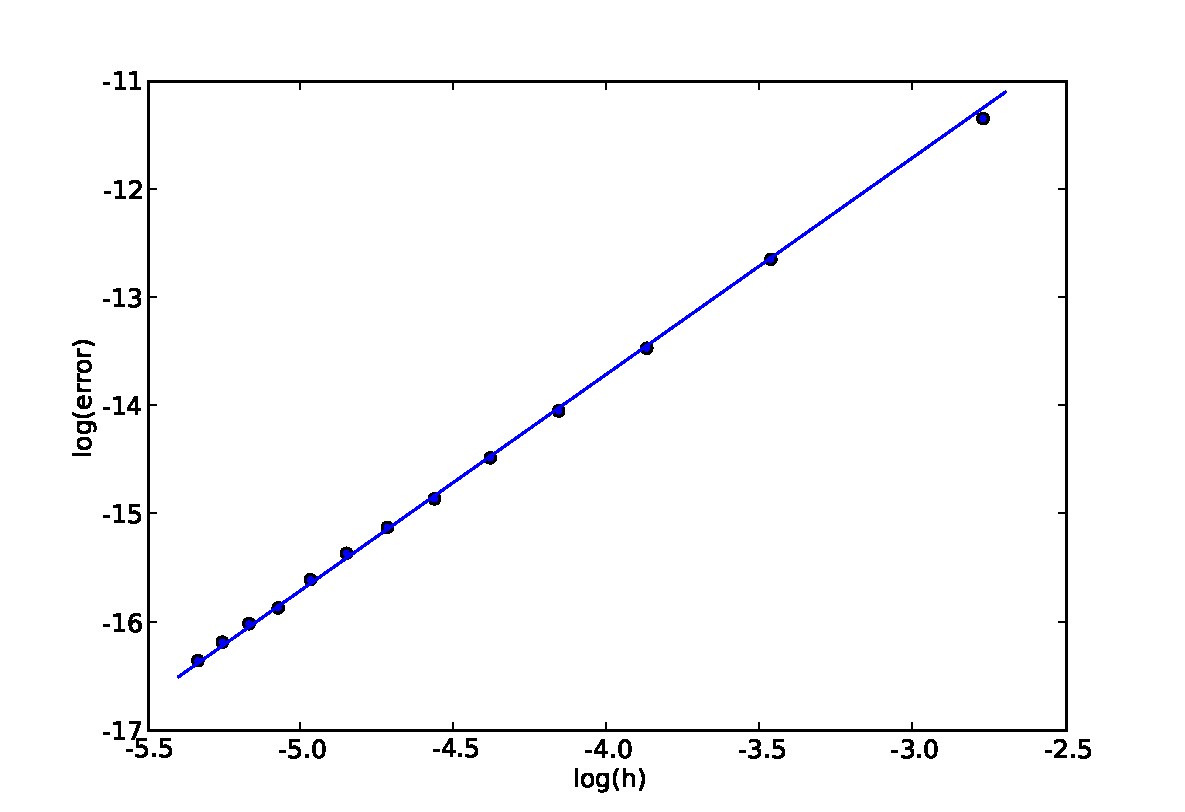
\includegraphics[bb=0in 0in 7.7in 6.3in,width=4.8in,clip]{Images_Methodology/matrixerror.pdf}
  \end{center}
  \caption{\small Log-log plot of $\norm{M_n-\tilde{M}_n}_\infty$ with $\Delta t = h$. The continuous line is a fit with a line of slope 2.}
  \label{fig:loglog15}
\end{figure}




\subsection{Error estimate for approximation of the matrix representation of $\C{M}_n$ in 3D}
\label{sub:TranslationError_3D}
In the previous section it was shown that in 2D the error $|(G_h(\B{x},\B{y})-G_h(\B{x}-\B{y}))_{ij}|$ is smaller than $O(h)$. We sketch here the extension of this result to the 3D case.

First, we require a Green's function $g_h$ associated with the operator $\C{L}_h$. $G_h$, the Green's function relating the influence of one fiber point on another, can be written as a summation involving $g_h$. Bounds on $g_h$ will lead to bounds on the translation error associated with $G_h$.

We define three force fields
\begin{equation}
\B{f}_i(\B{x})_j = \begin{cases}
1/h^3& \textrm{if } \B{x} = \B{0}, i=j \\
0& \textrm{otherwise,}
\end{cases}
\end{equation}
for $i,j=1,2,3$. These force fields correspond to a suitably scaled point force along a cardinal direction centered at the origin. With these we define the $3\times 3$ tensor field
\begin{equation}
g_h(\B{x})_{ij} = \C{L}_h(\B{f}_i)_j.
\end{equation}
Following Lemma~\ref{lemma:gh} we may bound the components of $g_h$ via
\begin{equation}
\label{meq:IntegralBound}
\begin{split}
\norm{(g_h)_{ij}}_\infty &\leq
\sum %_{\B{k} \in \C{G}_F }
\frac{1}{1 + 16\nu\Delta t |\B{k}|^2} \\
&\leq C \int_0^{\frac{\sqrt{2}}{2}N}\frac{1}{1 + 16\nu\Delta t r^2}r^2\,dr
< C\frac{N}{\Delta t},
\end{split}
\end{equation}
where the sum is over the set $\{\B{k}\in\BB{Z}^3 \: | \,\: |\B{k}_i| < N/2\}$, and the integral is obtained from a spherical coordinate transformation.
%If $\Delta t \propto h$ then $\norm{(g_h)_{ij}}_\infty < C{\Delta t}^{-1}h^{-1}$.

Consider now two fiber points, located at $\B{x}$ and $\B{y}$. We wish to bound the tensor components of the error $G_h(\B{x},\B{y})-G_h(\B{x}-\B{y})$. By Theorem~\ref{thm:A} we have 
\begin{equation}
|(G_h(\B{x},\B{y})-G_h(\B{x}-\B{y}))_{ij}|
< 
\frac{2(\Delta t)^2}{\rho} \norm{(g_h)_{ij}}_\infty h_B.
\label{meq:TranslationBound_Preliminary_Again}
\end{equation}
Assuming $\Delta t \propto h$ and $h_B \propto h^2$, then (\ref{meq:TranslationBound_Preliminary_Again}) combined with (\ref{meq:IntegralBound}) gives us the bound
\begin{equation}
|G_h(\B{x},\B{y})-G_h(\B{x}-\B{y})|_{ij}
< 
C h^2,
\end{equation}
which is smaller than the $O(h)$ error of the IB Method.




\subsection{Additional considerations and optimizations concerning $\tilde{M}_n$}
There are a few additional optimizations possible when constructing $\tilde{M}_n$, the matrix representation of $\C{M}_n$.
Note first that on a square domain $\Omega$ we have via symmetry that
\begin{gather}
G_h(x,y)_{00} = G_h(y,x)_{11}, \\
G_h(x,y)_{01} = G_h(y,x)_{10}.
\end{gather}
On a cubic domain we have similar symmetries, such as 
\begin{gather}
G_h(x,y,z)_{00} = G_h(y,x,z)_{11} = G_h(z,y,x)_{22}, \\
G_h(x,y,z)_{01} = G_h(y,x,z)_{10} = G_h(x,z,y)_{02}.
\end{gather}
Using these symmetries we can reduce the size of the precomputed lookup table for $G_h$.
For rectangular or otherwise irregular grids these symmetries do not hold, we do however have other symmetries; most importantly $G_h(\B{x}) = G_h(-\B{x})$.
This symmetry implies that the matrix of $\C{M}_n$ is symmetric. This observation reduces the cost of computing the matrix roughly by half.

The cost could be reduced further if interpolation were not used between grid points when looking up $G_h(\B{z})$ for arbitrary $\B{z}$. Unfortunately, the resulting error introduced in the simulation would be significant. A simple compromise is to use linear interpolation when calculating $G_h(\B{z})$ if $\norm{\B{z}}_2$ is small and direct lookup otherwise. This is inexpensive, with only $O(N_B)$ interpolations needed, because most fiber points are distant from each other, as well as accurate, because $G_h$ decays rapidly away from the origin. 

Alternatively, we could employ an adaptive mesh on which to construct the lookup table for $G_h$, taking a dense grid around the origin where most of the structure lies. This would allow us to use direct lookup for all entries of $\C{M}_n$ without much loss of accuracy. We do not pursue these strategies here and only utilize the symmetry of the matrix of $\C{M}_n$ to expedite the construction. This shortcut was used in calculating the costs given in Table~\ref{Table:MConstruct}.






\section{Multigrid}
\label{Sec:Multigrid}
With an approximate matrix form of $\C{M}_n$ in hand we can now move beyond Krylov methods and consider alternative iterative methods to solve our implicit system (\ref{meq:Xnl}). In particular we can now easily implement Gauss-Seidel. In the case that $\C{A}_{h_B}$ is linear and negative-semidefinite we define $B=I - \C{M}_n\C{A}_{h_B}$, which itself is positive-definite. Our system (\ref{meq:Xnl}) is then just the matrix problem
\begin{equation}
B\B{X}^{n+1} = \B{b}^n. \label{meq:MatrixProblem}
\end{equation}
This problem is amenable to Gauss-Seidel and Successive over-relaxation (SOR). Unfortunately the number of iterations required to achieve adequate convergence is typically prohibitive. However, SOR functions well at reducing high frequencies errors, and is thus suitable as a smoother in a multigrid. In this section we overview briefly a simple multigrid implementation. We then show the results of numerical experiments detailing the efficiencies of the multigrid method.

For simplicity in presentation, we consider a simple elliptical interface immersed in a 2D fluid. For details of the multigrid method applied to a more complicated geometry see Section~\ref{Sec:valve}.

Suppose that $N_B=2^m$ for some natural number $m$. We can then form a collection of Lagrangian grids $\C{G}^l$, $l=1, \ldots m$, with number of nodes equal to $2^m,2^{m-1},  \ldots, 2,1$.
Our original grid corresponds to the first level, $l=1$, with coarser grids coming afterward.
For a given level $l$  of the multigrid hierarchy,  the prolongation operator $\C{P}_l$ takes a fiber $\B{X}_{l+1}$ at level $l+1$ and adds a node between each pair of consecutive nodes equidistant between each. As a matrix,  $\C{P}_l$ has dimensions $2\cdot 2^{m-l+1}\times 2\cdot 2^{m-l}$ and has the form
\begin{equation}
\C{P}_l = 
\left( \begin{array}{cccc}
1  & 0  & 0  &  \\
.5 & .5 & 0  & \dots \\
0  & 1  & 0  & \\
0  & .5 & .5 & \\
   &\vdots& & \ddots
\end{array} \right).
\end{equation}
Restriction operators are taken to be the transposes of prolongation operators. Calling $\C{K}_1 = (\mathit{I}- \C{M}_n\C{A}_{h_B})$ we define recursively $\C{K}_l = \C{P}_{l-1}^{\mathit{T}} \C{K}_{l-1} \C{P}_{l-1}$.
All together,  a single restriction, prolongation, and smoothing step looks like
\begin{itemize}
\item Given a guess $\B{X}_l$ to the linear problem
\begin{equation}
\C{K}_l\B{X}_l = \B{b}_l 
\end{equation}
calculate the residual and restrict it to the next lowest level
\begin{equation}
\tilde{\B{r}}_{l+1} = \C{P}_l^T(\B{b}_l - \C{K}_l\B{X}_l)
\end{equation}
\item Find the correction on the coarse grid by solving or approximating
\begin{equation}
\C{K}_{l+1}\B{X}_{l+1} = \tilde{\B{r}}_{l+1}
\end{equation}
\item Correct our initial guess
\begin{equation}
\B{X}_l \leftarrow \B{X}_l + \C{P}_l \B{X}_{l+1}
\end{equation}
\item Smooth the high frequency errors in $\B{X}_l$ via SOR.
\end{itemize}
The number of iterations needed depends more on the desired degree of accuracy than a requirement for stability. Typically a single iteration of a Full Multigrid Step with one V-cycle per level is sufficient to maintain stability. 



\subsection{Case I: An initially elliptical drop with linear $\C{A}_{h_B}$}
\label{Sec:drop}
We consider as our first example what has been the canonical test for methods intended to remove the severe stiffness of the IB method. This is the case of a closed, continuous membrane $\B{X}(s,t)$ with a force distribution given by $\C{A}(\B{X})=\sigma\B{X}_{ss}$, where $\sigma$ is a (large) constant. We take our domain as $\Omega = [0,1]\times[0,1]$ with periodic boundary conditions and we fix $\mu=\rho=1$. Initially, we have an elliptical drop and zero velocity and the drop relaxes toward the equilibrium configuration. Figure~\ref{fig:Ellipse} shows the initial and final configurations of the interface.

We discretize $\C{A}(\B{X})$ as
\begin{equation}
\left(\C{A}_{h_B}\B{X}\right)_i = \frac{1}{h_B^2}\left(\B{X}_{i+1}-2\B{X}_i+\B{X}_{i-1}\right),
\label{eqn:LinearForce}
\end{equation}
where we have omitted the parentheses in the discrete force operator $\C{A}_{h_B}$ to emphasize that it is linear.
\begin{figure}[!b]
  \begin{center}
    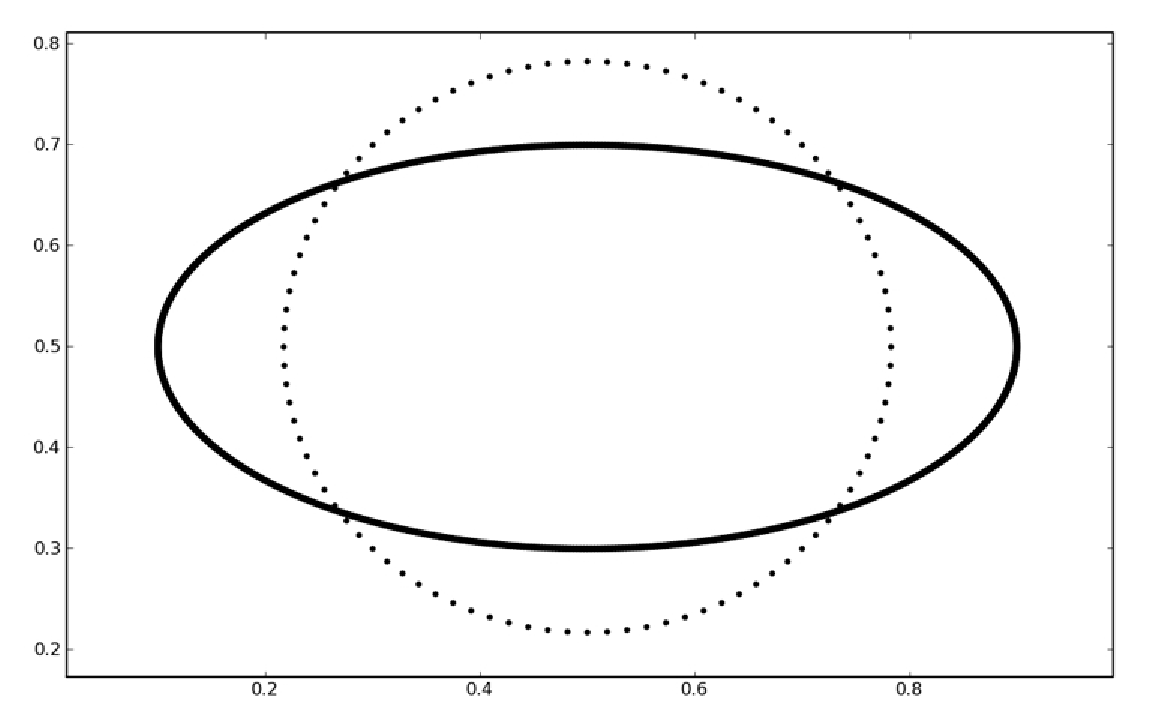
\includegraphics[bb=0in 0in 7.7in 4.8in,width=4.8in,clip]{Images_Methodology/Ellipse.pdf}
  \end{center}
  \caption{\small Initial configuration of fiber in bold and final rest configuration in dotted line.}
  \label{fig:Ellipse}
\end{figure}

We set the elasticity constant $\sigma=10^5$ and take $N_B = 2N$. The initial configuration of the fiber is an ellipse given by
\begin{equation}
\B{X}(s,0) = (0.5 + 0.3\cos(2\pi sh_B), 0.5 + 0.2\sin(2\pi sh_B)),
\end{equation}
for $s \in [0,1]$.
As time elapses,  the interfacial tension drives the ellipse toward a circular (cylindrical) configuration. The velocity of the fiber can reach roughly $500$ units before it slows down toward equilibrium. Taking a standard length to be the geometric mean of our radii, $0.245$, we calculate the Reynolds number of our fluid to be approximately $100$.


\subsection{Case I: Numerical results}
Solving our implicit system (\ref{meq:dmoment})-(\ref{meq:Xt}) via the multigrid described in Section~\ref{Sec:Multigrid} has five primary costs.
\begin{enumerate}
\item First, when constructing the implicit system (\ref{meq:Xnl}) we must calculate $\B{b}^n$ via a fluid solve, with a cost of roughly one FE/BE.
\item Second, the cost of constructing the approximate matrix form of $M_n$ is roughly one half FE/BE.
\item Third is the cost of initializing the multigrid solver, i.e. calculating the coarse representations of $M_n$ on the various levels of our grid. Use of sparse data structures is critical here to maintain $O(N_B^2)$ cost.
\item Fourth, is the cost of our iterations to solve the linear system. Because matrix-vector multiplication is significantly cheaper than FE/BE (see Table~\ref{Table:MV}) a full multigrid step can be much more economical than one FE/BE and this advantage grows  as $N$ increases.
\item The final cost is in computing $\B{u}^{n+1}$ once $\B{X}^{n+1}$ is known. This step involves another fluid solve with a cost of roughly one FE/BE.
\end{enumerate}    
We will see that the sum of these costs for the semi-implicit method results in a single time-step that costs approximately 4 FE/BE. However, the stability restraint on $\Delta t$ for the FE/BE scheme for a stiff problem like this one is orders of magnitude smaller than that required by the semi-implicit discretization. Thus, our proposed approach yields a much superior computational strategy.


As a reference for comparison, for fiber-explicit simulations we use the FE/BE scheme 
 with $\Delta t$ as large as  stability permits, which we find to be approximately $\Delta t = 0.00025h$. For our implicit scheme we make use of a linear multigrid with stopping criteria of $\norm{\B{r}^k}_{\infty}<30\Delta t$, where $\B{r}^k$ is the residual $\B{b}^n-(I-M_n A_{h_B})\B{X}^{n+1,k}$ at the $k$th iterate and $\norm{\cdot}_{\infty}$ is the sup norm. Here $\Delta t$ is 
 chosen to comply with the CFL condition as the convection term is treated explicitly. With a conservative estimate for the maximum 
 velocity, the time-step is given approximately by $\Delta t = 0.02h$. 
 \begin{table}
\caption{Elliptical drop relaxation for Navier Stokes. The average CPU time per time-step and the total CPU time up to a simulation time of $T=0.005$ is given. $\Delta t$ is the time-step taken and is the maximum allowed while maintaining stability.}
\label{table:EllipseConvectiveSims}
\begin{center}
\begin{tabular}{|c |c c c| c c c|}
\hline
& \multicolumn{3}{c|}{Explicit} & \multicolumn{3}{c|}{Implicit}\\
$N$ & $\Delta t$ & Average & Total & $\Delta t$ & Average & Total\\
\hline
128 & $1.95\cdot 10^{-6}$ & 0.03 & 73.35 & $1.17\cdot 10^{-4}$ & 0.10 & 4.34 \\
256 & $9.76\cdot 10^{-7}$ & 0.14 & 730.21 & $7.81\cdot 10^{-5}$ & 0.55 & 35.06\\
384 & $6.51\cdot 10^{-7}$ & 0.34 & 2613.19 & $5.21\cdot 10^{-5}$ & 1.24 & 118.98\\
512 & $4.87\cdot 10^{-7}$ & 0.63 & 6491.95 & $3.91\cdot 10^{-5}$ & 2.34 & 299.10\\
\hline
\end{tabular}
\end{center}
\end{table}

The results of multiple simulations with varying $N$ for the explicit and implicit methods are given in 
Table~\ref{table:EllipseConvectiveSims}. The rows in the table correspond to identical simulation runs with different $N$. The columns under the title Explicit relate data from the FE/BE simulations, whereas the Implicit columns relate data from the implicit simulations. The two columns marked Average give the average CPU time of a single timestep. The columns marked Total give total CPU time for the entire simulation, up to a simulation time of $T=0.005$.


We see in Table~\ref{table:EllipseConvectiveSims}
that the implicit scheme costs approximately $4$ times as much per time-step than FE/BE. However, because $\Delta t$ can be taken up to the CFL restraint, the scheme is roughly $20$ times faster than the explicit scheme in terms of total CPU time. 
Here, the performance of the semi-implicit approach is limited by the presence of large convection (relative to  viscous dissipation). Of course, one could employ a suitable implicit discretization of the convection terms to remove the CFL constraint.  Effective options in this context have been proposed by
Mori and Peskin~\cite{MP2008} and Hou and Shi~\cite{HS2008b}. We do not pursue this 
here as our intent is to focus on the treatment of the tension forces. Alternatively, if we consider Stokes flow the semi-implicit method
is no longer limited by a CFL restriction and we can take arbitrarily sized time-steps  while maintaining stability.
We compare the performance of the two methods for Stokes flow in Table~\ref{table:EllipseStokesSims}. 

In these simulations we have increased the total simulation time to $T = .05$. This simulation time is enough that the explicit methods may require unreasonable amounts of CPU time. We approximate the total CPU time for these longer simulations by calculating the average CPU time of a single timestep and multiplying by the number of timesteps the explicit simulation would require to complete. We use an asterisk here and in following tables to denote values based on these extrapolated values.

While $\Delta t$ for our implicit simulation can be chosen with disregard to stability, care must still be taken to ensure accuracy. Here we only require the loose condition that $\Delta t < h$. This is sufficient to preserve the qualitative behavior of our immersed structure. We note that there are implicit discretizations of the IB method with higher order accuracy in time, see for example \cite{NFGK2007}. Many of these methods require very little additional work to implement and do not require much additional CPU time per timestep. These methods may allow IB simulations to maintain high accuracy while exploiting the large timesteps allowed by an implicit discretization.

\begin{table}
\caption{Ellipse relaxation for Stokes flows. The average CPU time per timestep and the total CPU time up to a simulation time of 
$T=0.05$ is given. $\Delta t$ is the timestep taken. For the explicit scheme this is the maximum allowed while maintaining stability. The implicit scheme is unconditionally stable; the timestep taken is held constant as $N$ varies.  $^*$ denotes an extrapolated value.}
\label{table:EllipseStokesSims}
\begin{center}
\begin{tabular}{|c |c c c| c c c|}
\hline
& \multicolumn{3}{|c|}{Explicit} & \multicolumn{3}{|c|}{Implicit}\\
$N$ & $\Delta t$ & Average & Total & $\Delta t$ & Average & Total\\
\hline
128 & $1.95\cdot 10^{-6}$ & 0.03 & 683.96 & $0.001$ & 0.09 & 9.34\\
256 & $9.76\cdot 10^{-7}$ & 0.15 & 7410.50 & $0.001$ & 0.53 &  53.08\\
384 & $6.51\cdot 10^{-7}$ & 0.35 & $26555.30^*$ & $0.001$ & 1.24 & 123.86\\
512 & $4.87\cdot 10^{-7}$ & 0.71 & $72669.41^*$ & $0.001$ & 2.32 & 232.05\\
\hline
\end{tabular}
\end{center}
\end{table}



\subsection{Case II: An initially elliptical drop with nonlinear $\C{A}_{h_B}$}
\label{Sec:Nonlinear}
We consider now the case of the simple, initially elliptical membrane  with a nonlinear force and detail how to adapt the method from the previous linear case.

We follow Mori and Peskin in \cite{MP2008} for the setup of this nonlinear $\C{A}_{h_B}$  example. At the continuous level,  the fiber force distribution is given by
\begin{equation}
\B{F} = \frac{\partial}{\partial s} (T\B{t})
\end{equation}
where $\B{t}(s,t)$ is the tangential unit vector to $\B{X}(s,t)$ and $T(s,t)$ is the tension given by
\begin{equation}
T(s,t) = \left| \frac{\partial\B{X}}{\partial s}(s,t) \right|
 +     \left| \frac{\partial\B{X}}{\partial s}(s,t) \right|^2.
\end{equation}
To discretize this interfacial force we introduce the following difference operators for  a function $f$ defined over $\C{G}_B$:
\begin{eqnarray}
D_s^+f(s) = \frac{f(s+1)-f(s)}{h_B},\\
D_s^-f(s) = \frac{f(s)-f(s-1)}{h_B}.
\end{eqnarray}
We then define the discrete force distribution as
\begin{equation}
\B{F} = D_s^+ \left(\left(
\left| D_s^-\B{X} \right| +
\left| D_s^-\B{X} \right|^2 \right)
\frac{ D_s^-\B{X} }{ \left| D_s^-\B{X} \right| } \right).
\end{equation}
Severe stiffness in this model is manifested when the interfacial elastic force is much larger than the viscous forces. Following
Mori and Peskin~\cite{MP2008} we set $\rho = 1$ and either $\mu = .05$ or $\mu = .005$. As before the domain is $\Omega = [0,1]\times[0,1]$ which we discretize as $\Omega_h$, an $N\times N$ uniform Eulerian grid. As in the linear case, the initial velocity of the fluid is zero everywhere. The fiber's initial configuration is given by
\begin{equation}
\B{X}(s,0) = (\frac{1}{2} + \frac{1}{3}\cos(2\pi sh_B), \frac{1}{2} + \frac{1}{4}\sin(2\pi sh_B)).
\end{equation}
With our implicit strategy we attempt to solve at each time step the {\em nonlinear} system (\ref{meq:Xnl})
$$
\B{X}^{n+1} = \C{M}_n\C{A}_{h_B} (\B{X}^{n+1}) + \B{b}^n,
$$
where $\C{M}_n$ and $\B{b}^n$ are as in the linear case. We could simply approximate $\C{A}_{h_B}$ linearly and solve the resulting linear system. This is easily accomplished because the Jacobian $J$ of $\C{A}_{h_B}$ is negative semidefinite, hence  $I-\C{M}_nJ$ is positive definite. Such linear approximation is simple and reasonably robust
but not as stable as the implicit scheme with full nonlinear term. This linear approximation is the method employed by Mori and Peskin~\cite{MP2008} for their first order scheme. However, with our economical computational approach we can afford the extra stability (while maintaining accuracy) by solving the nonlinear system (\ref{meq:Xnl}) via Newton iterations. Specifically, at each time-step we perform Newton iterations until the sup norm of the residual is less than $10^{-4}$. This typically requires only $2$ or $3$ iterations. Note that a single iteration per timestep would be identical to the linear approximation used by Mori and Peskin. We expedite further the 
computation by approximating the solution to the linear system at each one of Newton's iteration with 3 Multigrid cycles.

\subsection{Case II: Numerical results}
We choose this nonlinear test problem following Mori and Peskin ~\cite{MP2008} to have their results as a reference. However, 
there is a  slight difference in the model in addition to the different discretizations employed; Mori and Peskin use an immersed fiber with finite mass while our own fiber is neutrally buoyant.  We present the results from our numerical experiments in a format similar to that presented in~\cite{MP2008} to facilitate comparisons.

Let $N_T$ be the number of timesteps taken, with total simulation time fixed at $1$. We fix $N_B=2N$ as before. 
Table~\ref{table:NonlinearEllipseSims_05Fluids}, for $\mu=0.05$, and Table~\ref{table:NonlinearEllipseSims_005Fluids}, 
for $\mu=0.005$,  summarize the total computational cost in units of FE/BE's. The total CPU time for the same cases is displayed in
  Table~\ref{table:NonlinearEllipseSims_05CPU} and Table~\ref{table:NonlinearEllipseSims_005CPU}, respectively.
  In all four tables the columns under FE/BE hold the explicit result while the columns under $N_T=8$ and $N_T=16$ hold the implicit results, with $N_T$ as specified. 

As noted in~\cite{MP2008}, the semi-implicit method becomes more efficient compared to the explicit (FE/BE) 
scheme as $N$ increases and $\mu$ decreases (more stiffness). For $N_T=8$ and $N=512$ the proposed semi-implicit strategy is about 45 times faster than the explicit approach in the case of $ \mu=0.05$ and about 90 times faster for $\mu=0.005$. In contrast, the fully implicit
approach in~\cite{MP2008} gives cost ratios in the range $12-16$ for the same parameters.


\begin{table}
\caption{Total CPU cost for the nonlinear ellipse model with $\mu=0.05$. Values given are total CPU time divided by average CPU time of a single FE/BE timestep for the given $N$.}
\label{table:NonlinearEllipseSims_05Fluids}
\begin{center}
\begin{tabular}{|c|c| c c|}
\hline
$N$ & FE/BE & $N_T = 8$ & $N_T = 16$\\
\hline
$64$ & $166$ & $38.2$ & $75.5$ \\
$128$ & $500$ & $49.7$ & $89.7$ \\
$256$ & $1333$ & $53.0$ & $97.2$ \\
$512$ & $2666$ & $59.3$ & $92.6$ \\
\hline
\end{tabular}
\end{center}
%\end{table}

%\begin{table}
\caption{Total CPU cost for the nonlinear ellipse model with $\mu=0.005$. Values given are total CPU time divided by average CPU time of a single FE/BE timestep for the given $N$.}
\label{table:NonlinearEllipseSims_005Fluids}
\begin{center}
\begin{tabular}{|c|c| c c|}
\hline
$N$ & FE/BE & $N_T = 8$ & $N_T = 16$\\
\hline
$64$ & $333$ & $83.5$ & $112.4$ \\
$128$ & $1000$ & $74.8$ & $113.1$ \\
$256$ & $2666$ & $71.7$ & $112.6$ \\
$512$ & $5333$ & $59.2$ & $101.9$ \\
\hline
\end{tabular}
\end{center}
\end{table}

\begin{table}
\caption{Total CPU time for the nonlinear ellipse model with $\mu=0.05$.}
\label{table:NonlinearEllipseSims_05CPU}
\begin{center}
\begin{tabular}{|c|c| c c|}
\hline
$N$ & FE/BE & $N_T = 8$ & $N_T = 16$\\
\hline
$64$ & $2.94$ & $0.67$ & $1.33$ \\
$128$ & $20.89$ & $2.08$ & $3.75$ \\
$256$ & $227.85$ & $9.05$ & $16.59$ \\
$512$ & $1930.62$ & $42.94$ & $67.02$ \\
\hline
\end{tabular}
\end{center}
\end{table}

\begin{table}
\caption{Total CPU time for the nonlinear ellipse model with $\mu=0.005$.}
\label{table:NonlinearEllipseSims_005CPU}
\begin{center}
\begin{tabular}{|c|c| c c|}
\hline
$N$ & FE/BE & $N_T = 8$ & $N_T = 16$\\
\hline
$64$ & $5.31$ & $1.33$ & $1.79$ \\
$128$ & $42.06$ & $3.14$ & $4.75$ \\
$256$ & $455.11$ & $12.24$ & $19.22$ \\
$512$ & $3823.40$ & $42.45$ & $73.10$ \\
\hline
\end{tabular}
\end{center}
\end{table}


\section{Conclusion}
In this chapter we developed a novel methodology for efficiently solving implicit discretizations of the IB Method, namely the matrix method and the resulting multigrid. We showed that for certain simple applications we can efficiently remove the stiffness in the IB Method and drastically decrease the computational cost of simulations. In Chapter~\ref{part:Splitting}, we will show that the matrix method is amenable to much more complex problems.

\subsection{Strengths of the matrix method}
When should the matrix method be used? Certainly in the case of a 2D fluid there are many potential applications. If $N_B \ll N^2$ then a large savings can be had by forming an approximate matrix representation of $\C{M}_n$ at each timestep. This savings is present regardless of whether the implicit system is amenable to multigrid.

When applicable, however, multigrid is a powerful solver. Provided that $\C{A}_{h_B}$ or its Jacobian matrix is negative-semidefinite then we can efficiently solve (\ref{meq:Xnl}) via multigrid, with the multigrid used inside a Newton iteration in the case that $\C{A}_{h_B}$ is nonlinear. In Chapter~\ref{part:Splitting} we will extend the methodology for a class of cases where the Jacobian is non-definite.


\subsection{Limitations of the matrix method}
While there are many advantages to the matrix method in 2D, the advantages disappear in a 3D application. If our immersed structure is a 2D membrane we would have $N_B \sim N^2$ leading to a cost of  $O(N^4)$ for a matrix-vector multiplication using the matrix  while obtaining the same product via spreading-fluid solver-interpolation would be $O(N^3\log N)$. Indeed, some 3D applications may use substantially more fiber points. The heart model proposed in~\cite{McQueenPeskin2000} employs nearly $N_B  \sim N^3$ fiber points. For such applications we will develop a different methodology, presented in Chapter~\ref{part:Treecode}.

We stress that it is very difficult to construct an efficient multigrid without the matrix method. Gauss-Seidel is prohibitively expensive, and alternative smoothers such as Jacobi iterations do not perform well. If a multigrid is to be employed then we will need to find an efficient means of calculating the Gauss-Seidel iteration. The treecode developed in Chapter~\ref{part:Treecode} allows for exactly this.






\chapter{The Treecode Method}
\label{part:Treecode}
\noindent
\section{Multipole summations and treecodes}
\label{Sec:Treecode}
Treecodes are efficient ways to evaluate certain sums. Suppose we have an expression of the form
\begin{equation}
\sum_{j=1}^{N_B} \phi(\B{X}_j, \B{X}_i) \B{F}_j,
\label{meq:Multipole}
\end{equation}
where $\{\B{F}_j\}_{j=1}^{N_B}$ is a collection of forces, and $\phi$ is some tensor valued potential.
Expression (\ref{meq:Multipole}) is referred to as a multipole summation. Evaluating (\ref{meq:Multipole}) for all $1\leq i\leq N_B$  directly requires $O(N_B^2)$ operations. However, treecodes can reduce the overall computational cost to $O(N_B\log N_B)$, provided  $\phi$ is sufficiently regular.

Given the function $G_h$, as constructed in Chapter~\ref{part:Matrix}, we can cast
our fluid evaluations as multipole summations of the form
\begin{equation}
(\C{M}_n\B{F})_i = \sum_{0\leq j\leq N_B} G_h(\B{X}_j - \B{X}_i) \B{F}_j.
\label{meq:IBMultipole}
\end{equation}
Calculating this sum directly is equivalent to the matrix method proposed in Chapter~\ref{part:Matrix}, and requires $O(N^4)$ operations when $N_B\sim N^2$.
The goal now is to apply a treecode algorithm to accelerate the evaluation of this sum, ideally reducing the cost from $O(N_B^2)$ to $O(N_B\log N_B)$. In the following two subsections we overview the basics of treecodes. We will elaborate in Section~\ref{Sec:Treecode_Expansions} on the far field expansions of $G_h$ that enable a treecode strategy to perform well for our particular problem. Following that we will detail two applications of the treecode method in Section~\ref{sec:KrylovMethods}.



\subsection{Overview}
For those unfamiliar with treecodes we briefly review the main ideas here. We recommend an alternative  exposition by Li, Johnston, and Krasny in~\cite{TreeCode_Krasny}. We also present a more detailed and technical overview of the treecode algorithm in Section~\ref{Sec:TreecodeDetails}.

The general strategy is to make use of far field expansions of $G_h$ to compress the outgoing effect of clusters of fiber points. Assume we have two subsets of our domain $\Omega$, $\Omega_{in}$ and $\Omega_{out}$, such that $G_h$ has a valid expansion in $\Omega_{in}\times \Omega_{out}$ given by
\begin{equation}
G_h(\B{x}-\B{y}) \approx \sum_{k=1}^{p}A_k(\B{x})B_k(\B{y}), \qquad \text{for $\B{x}\in\Omega_{in}$ and  $\B{y}\in\Omega_{out}$}.
\label{meq:Expansion}
\end{equation}
$\Omega_{out}$ serves to restrict the location of our pole, the \textit{outgoing} influence, while $\Omega_{in}$ serves to restrict the point of evaluation, the \textit{incoming} position.
Our expansion terms $\{A_k\}_{k=1}^p$ and $\{B_k\}_{k=1}^p$ are collections of $3\times 3$ matrix (tensor) fields defined on $\Omega_{in}$ and $\Omega_{out}$ respectively, with multiplication between two tensors defined componentwise, and multiplication between a tensor and a vector defined via the usual matrix-vector multiplication. If we further define
\begin{gather}
B_{in} = \{1 \leq i \leq N_B | \B{X}_i \in \Omega_{in}\}, \\
B_{out} = \{1 \leq i \leq N_B | \B{X}_i \in \Omega_{out}\},
\end{gather}
then we can consider the subproblem of calculating the influence of all the fiber points in $\Omega_{out}$ on the fiber points in $\Omega_{in}$:
\begin{equation}
\sum_{j\in B_{out}} G_h(\B{X}_i - \B{X}_j) \B{F}_j, \qquad\text{for $i\in B_{in}$}.
\label{meq:SubProblem}
\end{equation}
Calculating this summation for all $i$ in $B_{in}$ requires $O(|B_{in}|\cdot |B_{out}|)$ operations, where $|\cdot|$ denotes the number of elements in a set. We seek to reduce this cost.
Substituting (\ref{meq:Expansion}) in (\ref{meq:SubProblem}) yields
\begin{eqnarray}
\sum_{j\in B_{out}} G_h(\B{X}_j - \B{X}_i) \B{F}_j
&\approx \full\sum_{j\in B_{out}} \left( \sum_{k=1}^{p}A_k(\B{X}_i)B_k(\B{X}_j) \right)  \B{F}_j \nonumber \\
&= \B{E}^T\full\sum_{k=1}^{p}A_k(\B{X}_i) \sum_{j\in B_{out}} B_k(\B{X}_j) \tilde{F}_j.
\label{meq:SummingTrick}
\end{eqnarray}
Here $\tilde{F}_j$ is a $3\times 3$ matrix (tensor) where $(\tilde{F}_j)_{ab}=(\B{F}_j)_b$ and $\B{E}$ is a 3-vector whose components are all one. The additional complication of defining $\tilde{F}_j$ arises because the product of $A_k$ and $B_k$ in (\ref{meq:Expansion}) is understood  component-wise. The vector $\B{E}$ serves to collapse the final sum into a vector.


The summation over $B_{out}$ in (\ref{meq:SummingTrick}) may be calculated independently of $i$. Thus, given
\begin{equation}
H_k \equiv \sum_{j\in B_{out}} B_k(\B{X}_j) \tilde{F}_j,
\label{meq:CombinedFarField}
\end{equation}
we can efficiently calculate (\ref{meq:SubProblem}) via
\begin{equation}
\B{E}^T\full\sum_{k=1}^{p}A_k(\B{X}_i)H_k, \qquad\text{for $i\in B_{in}$}.
\label{meq:Compressed}
\end{equation}
Using (\ref{meq:Compressed}) to compute (\ref{meq:SubProblem}) requires $O(p|B_{in}| + |B_{out}|)$ operations, which may be substantially fewer than $O(|B_{in}|\cdot |B_{out}|)$ if $p\ll |B_{out}|$. This compression is one of the main ingredients of a treecode. The remaining difficulty is that $\Omega_{in}$ and $\Omega_{out}$ generally do not cover our entire domain. There may be fiber points $\B{X}_i$ and $\B{X}_j$ where $i,j$ do not belong to $B_{out},B_{in}$, hence the interaction between $\B{X}_i$ and $\B{X}_j$ would not be accounted for in (\ref{meq:SubProblem}).

To remedy this we must choose multiple pairs of $\left(\Omega_{in},\Omega_{out}\right)$ so that every ordered pair of fiber points $\left(\B{X}_i, \B{X}_j\right)$ is represented exactly once. This is essentially an organizational problem, and the standard procedure is to use binary space partitioning. In 3D this is known as an octree whereas in 2D  it is called a quadtree.

\subsection{The octree}
An octree is constructed by successively subdividing our domain $\Omega = [0,1]^3$ into smaller cubic domains called {\em panels}. 
Starting with the domain itself, called the {\em Root Panel},  we divide it into eight equal octants called child panels (of the root)
then recursively we define the eight children of each of those child panels and so on. This subdivision process is stopped for a panel which has fewer that an (arbitrarily set) minimum number of fiber points (10 here). 

The totality of the Root Panel  and all of its branches is collectively known as the octree. Visualizing an octree in 3D is difficult. For demonstrative purposes we present  in Figure~\ref{fig:PanelDecomp} a drawing of a quadtree in 2D.
\begin{figure}[!b]
  \begin{center}
    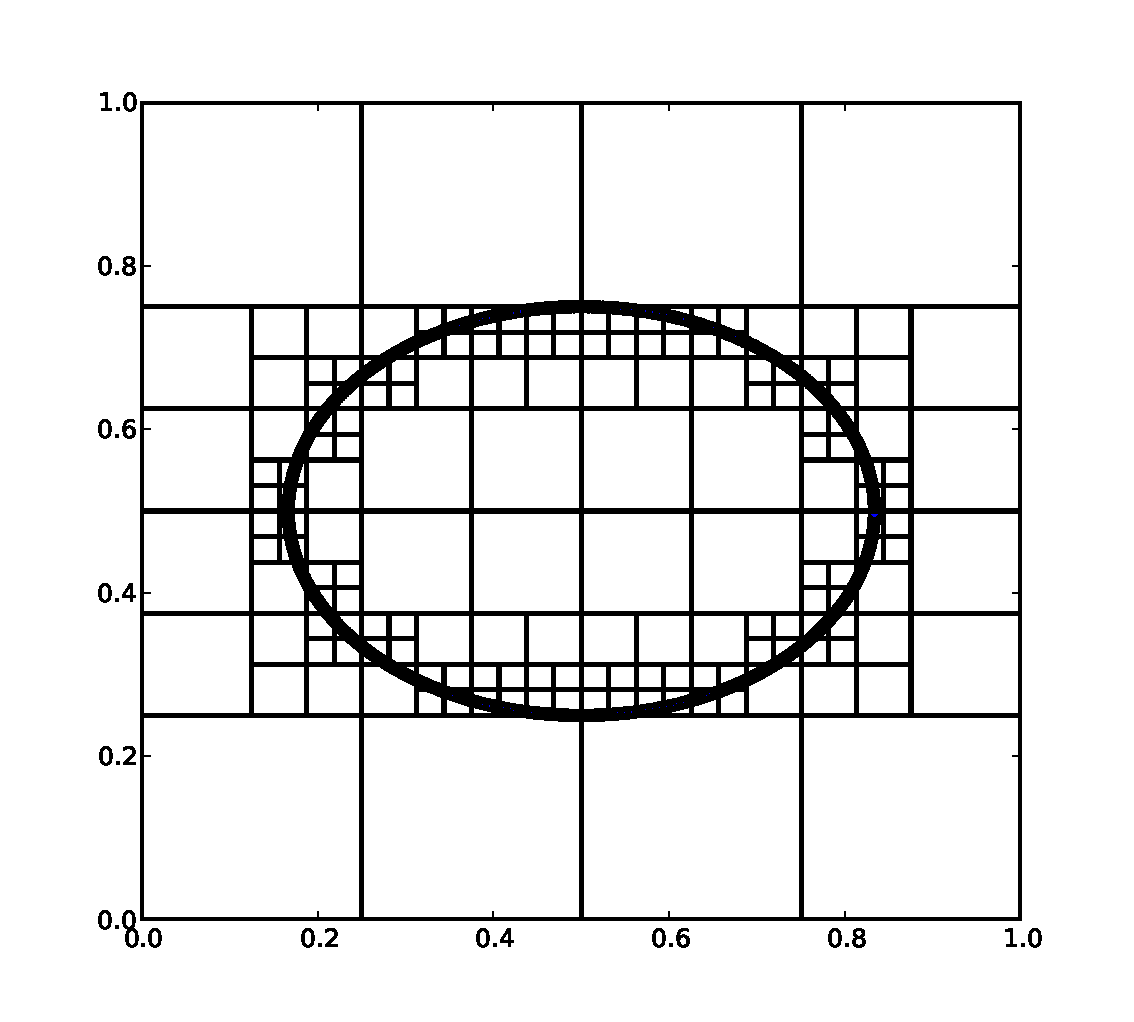
\includegraphics[bb=0in 0in 7.7in 6.3in,width=4.8in,clip]{Images_Methodology/Panels.pdf}
  \end{center}
  \caption{\small An ellipse shaped fiber $\B{X}$, with a quadtree decomposition of the space $[0,1]\times [0,1]$ containing it.}
  \label{fig:PanelDecomp}
\end{figure}

Given a panel $P$ we refer to its domain as $\Omega_{out}^P$.
A point $\B{x}$ is {\em well-separated} from a panel $P$ if  its  distance to the center of the panel is at least 3/2 the size of the panel [see~(\ref{ws})].
We refer to the domain of all points well-separated from $P$ as $\Omega_{in}^P$.
We assume that points in $\Omega_{in}^P$ are sufficiently far from $P$ that a multipole expansion could be used to calculate the effect of the {\em outgoing} influence of all the fiber points in $P$.  This assumption is equivalent to assuming that we can expand $G_h$ over $\Omega_{in}^P\times\Omega_{out}^P$, arriving at two collections of coefficient functions $\{A_k^P\}_{k=1}^p$ and $\{B_k^P\}_{k=1}^p$. 

Suppose now that we are given a fiber force $\B{F}$ and wish to evaluate its influence at points $\B{x}$ in the fluid domain. For each $\B{x}$ this influence is given by
\begin{equation}
\sum_{1\leq j\leq N_B} G_h(\B{x} - \B{X}_j) \B{F}_j.
\end{equation}
To evaluate this efficiently, we first loop over each panel $\Panel{P}$ and calculate the far field expansion of all the poles located in 
$\Panel{P}$. The $k$-th term of this expansion is given by
\begin{equation}
H_k^P \equiv \sum_{j\in B_{out}^P}
B_k^P(\B{X}_j) \tilde{F}_j.
\label{meq:Outgoing}
\end{equation}
If $\B{x}$ is well separated from $\Panel{P}$, then the incoming effect on $\B{x}$ from $\Panel{P}$ is given by
\begin{equation}
\B{E}^T \full\sum_{k=1}^{p}A_k^P(\B{X}_i)H_k^P.
\label{meq:Incoming}
\end{equation}
We can now evaluate the entire influence of $\B{F}$ on a point $\B{x}$, recursively.   We start with the panel $\Panel{P}=\Panel{Root}$. If $\B{x}$ is well separated from $\Panel{P}$ then we evaluate the influence of $\Panel{P}$ on $\B{x}$ via (\ref{meq:Incoming}). Otherwise, if $\Panel{P}$ has children we recursively apply this process to those child panels. If instead $\Panel{P}$ is childless, we directly evaluate the influence of every fiber point in $\Panel{P}$ on $\B{x}$, using (\ref{meq:SubProblem}). Summing all these influences from every branch of the recursion provides the desired total influence on $\B{x}$.

Note that (\ref{meq:Outgoing}) only needs to be calculated once per panel, and may be reused for calculating the influence at multiple points $\B{x}$. Because each fiber point $\B{X}_i$ is contained in at most $\log N$ panels, the total cost of computing $H_k^P$ for all panels $\Panel{P}$ is at most $O(N_B\log N_B)$. Calculating the influence at a given $\B{x}$ involves at most $O(\log N)$ panels, and hence the cost is at most $O(p\log N)$. The total cost of evaluating $\C{M}_n\B{F}$ is thus $O(pN_B\log N_B)$.

A detailed description of the octree creation and point evaluation is presented in~\ref{Sec:TreecodeDetails}.
\subsection{Expansions}
\label{Sec:Treecode_Expansions}
In order to make use of a treecode we must be able to find expansions (\ref{meq:Expansion}) of $G_h$ associated with particular pairs $\left(\Omega_{in},\Omega_{out}\right)$. Here, 
$G_h$ is a summation of discrete stokeslets. In free space, the continuous stokeslet has convenient analytic expansions useful for fast summation, see for instance~\cite{Stokes_FMM}. The same is not true for the discrete stokeslet corresponding to a periodic domain, and much less so for the particular summation of stokeslets that yields $G_h$. Fortunately, an analytic expansion is not indispensable in practice. What we seek are collections of tensor valued function $\{A_k\}_{k=1}^\Inf$ and $\{B_k\}_{k=1}^\Inf$ defined on $\Omega$ such that 
\begin{equation}
G_h(\B{x} - \B{y}) = \sum_{k = 1}^\infty A_k(\B{x}) B_k(\B{y}),
\end{equation}
and, moreover, such that truncating the above expansion to $p$ terms yields an adequate approximation, provided that $\B{x}$ and $\B{y}$ are well separated in some sense. That is, given two disjoint subsets $\Omega_{in}$ and $\Omega_{out}$ of our domain, we hope that for some small value of $p$ and for a specified tolerance $\epsilon$ that
\begin{equation}
\norm{
\left(G_h(\B{x} - \B{y}) - \sum_{k = 1}^p A_k(\B{x}) B_k(\B{y})\right)
\B{f}
}_2 < \epsilon \norm{\B{f}}_2,
%\text{ for $\B{x}\in\Omega_{in},\B{y}\in\Omega_{out}$},
\label{meq:Accuracy}
\end{equation}
for all $\B{f}\in\BB{R}^3$, $\B{x}\in\Omega_{in}$, and $\B{y}\in\Omega_{out}$.
%For our needs we will take $\epsilon\sim h$, the order of our discretization.

For a given $p$, finding the optimal expansion that allows for the smallest $\epsilon$ that satisfies (\ref{meq:Accuracy}) for all $\B{f},\B{x},\B{y}$ is an open question, and is likely computationally intractable.

We solve instead a least squares problem. We will search for the individual components of our tensors separately. Looking at each $ab$ components, for $a,b=x,y,z$, we seek the expansion coefficients $\{(A_k)_{ab}\}_{k=1}^p$ and $\{(B_k)_{ab}\}_{k=1}^p$ such that we minimize the $L^2$-norm of the difference between $G_h$ and our approximate expansion. That is, we seek to minimize
\begin{equation}
\norm{\left(G_h - \sum_{k = 1}^p A_k B_k\right)_{ab}}^2_2 \equiv
\iint
\left(G_h(\B{x} - \B{y}) - \sum_{k = 1}^p A_k(\B{x}) B_k(\B{y})\right)_{ab}^2
d\B{x} d\B{y},
\label{meq:L2Dif}
\end{equation}
where $A_k B_k$ is understood to be a function over $\Omega_{in}\times\Omega_{out}$, and the integrals are taken over $\B{x}\in\Omega_{in}$ and $\B{y}\in\Omega_{out}$. We approximate the integral in (\ref{meq:L2Dif}) as
\begin{equation}
\sum
\left(G_h(\B{x} - \B{y}) - \sum_{k = 1}^p A_k(\B{x}) B_k(\B{y})\right)_{ab}^2 h^6,
\label{meq:L2Dif_Sum}
\end{equation}
where the outer sum is taken over the Eulerian grid points in our subsets, $\B{x}\in\Omega_{in}\cap\C{G}_h$ and $\B{y}\in\Omega_{out}\cap\C{G}_h$.
Note that this minimization problem is decoupled with respect to the components of our tensors. We may thus consider the task of minimizing (\ref{meq:L2Dif_Sum}) as nine separate minimization problems.

It is useful to view our problem as a statement about matrices. To do this we first write $(G_h)_{ab}$ as an $N^3\times N^3$ matrix, which we refer to as $\ti{G}$ and which is given by the relation
\begin{equation}
\ti{G}_{ij} = G_h((j_0,j_1,j_2)h-(i_0,i_1,i_2)h),
\end{equation}
where $i = i_0 + i_1N + i_2N^2$ and $j = j_0 + j_1N + j_2N^2$ for any $0\leq i_l < N$, $0\leq j_l < N$, with $l=0,1,2$. We may likewise write $(A_k)_{ab}$ and $(B_k)_{ab}$ as $N^3$-vectors labeled $\ti{A}_k$ and $\ti{B}_k$.
We now stitch our collections of vectors $\{\ti{A}_k\}$ and $\{\ti{B}_k\}$ into matrices. Given $p$, we define an $N^3\times p$ matrix $U$, a $p\times N^3$ matrix $V$, and a $p\times p$ diagonal matrix $\Sigma$ via
\begin{equation}
U_{jk} = \frac{(\ti{A}_k)_j}{\norm{\ti{A}_k}_2},
\qquad
V_{kj} = \frac{(\ti{B}_k)_j}{\norm{\ti{B}_k}_2},
\qquad
\Sigma_{kk} = \norm{\ti{A}_k}_2 \norm{\ti{B}_k}_2,
\end{equation}
for $1\leq j\leq N^3$ and $1\leq k\leq p$.

The $p$ columns of $U$ are simply the normalized vector encodings of the $p$ coefficient functions $\{A_k\}_{k=1}^p$. The rows of $V$ are likewise formed from $\{B_k\}_{k=1}^p$.
Note that we may reorder our indices such that $\{\Sigma_{kk}\}_{k=1}^p$ is a decreasing sequence.

We can now express our sum (\ref{meq:L2Dif_Sum}) as $\norm{\ti{G}-U\Sigma V}_F^2h^6$, where $\norm{\cdot}_F$ is the Frobenius matrix norm. Minimizing the Frobenius norm here is a well-studied least squares problem. It is known that if we take $p=N^3$ and find the optimal expansion minimizing (\ref{meq:L2Dif_Sum}) then we recover $\ti{G}$ exactly. That is, $\ti{G} = U\Sigma V$. This is precisely the Singular Value Decomposition (SVD) of $\ti{G}$.

The key property of this decomposition for our needs is that, for a given $p<N^3$, truncating the SVD to $p$ terms provides the minimizing expansion for (\ref{meq:L2Dif_Sum}). That is, given the SVD of $\ti{G}$,
we can obtain the optimal $p$-term expansion coefficient functions $\left\{A_k\right\}_{k=1}^p, \left\{B_k\right\}_{k=1}^p$ from the first $p$ columns of $U\sqrt{\Sigma}$ and the first $p$ rows of $\sqrt{\Sigma}V$, respectively. This result is known as the Eckart-Young theorem~\cite{EckartYoung} and the resulting expansion is the so-called rank-1 decomposition.
%The phrase rank-1 decomposition is used to stress that the terms $A_i\otimes B_i$ are rank-1 functions.

Using this optimal $p$-term expansion, the $L^2$-error (\ref{meq:L2Dif_Sum}) is given by the square sum of the neglected singular values,
\begin{equation}
\left( \sum_{k=p+1}^{N^3}\Sigma_{kk}^2 \right)^{1/2}.
\end{equation}
The accuracy of our $p$-term expansion is thus directly related to the rate of decay of the singular values of $\ti{G}$. The faster the singular values decay the fewer terms we require in our expansion  to accurately capture the behavior of $\ti{G}$. Figure~\ref{fig:svalues_00} shows the sharp decay of the singular values of $\ti{G}$, where we have encoded in $\ti{G}$ the $xx$ and $xy$ components of $G_h$ respectively. It is this marked decay that allows for an efficient treecode approach.
\begin{figure}[htb]
	\begin{center}
		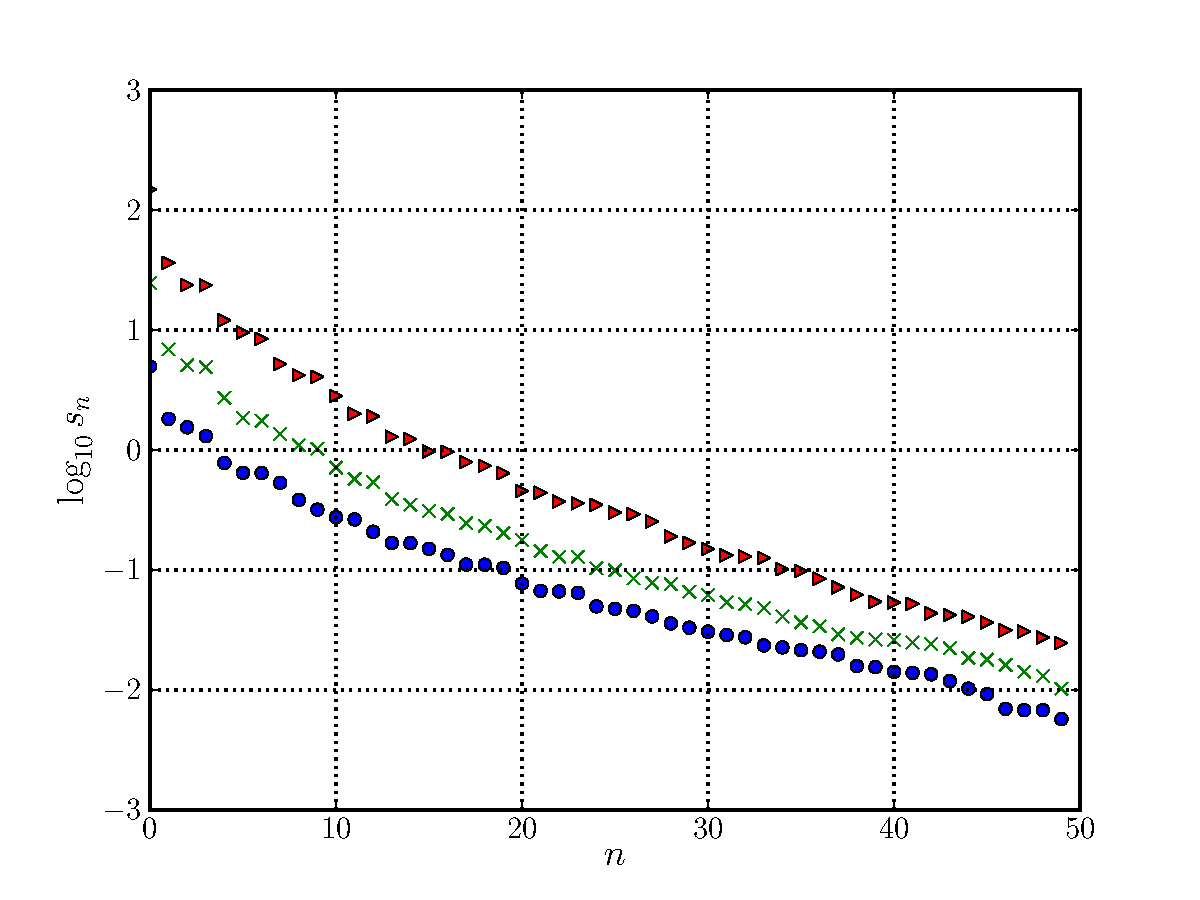
\includegraphics[bb=0in 0in 7.7in 6.3in,width=\StandardFigureWidth,clip]{Images_Methodology/svalues_00.pdf}
	\end{center}
	\begin{center}
		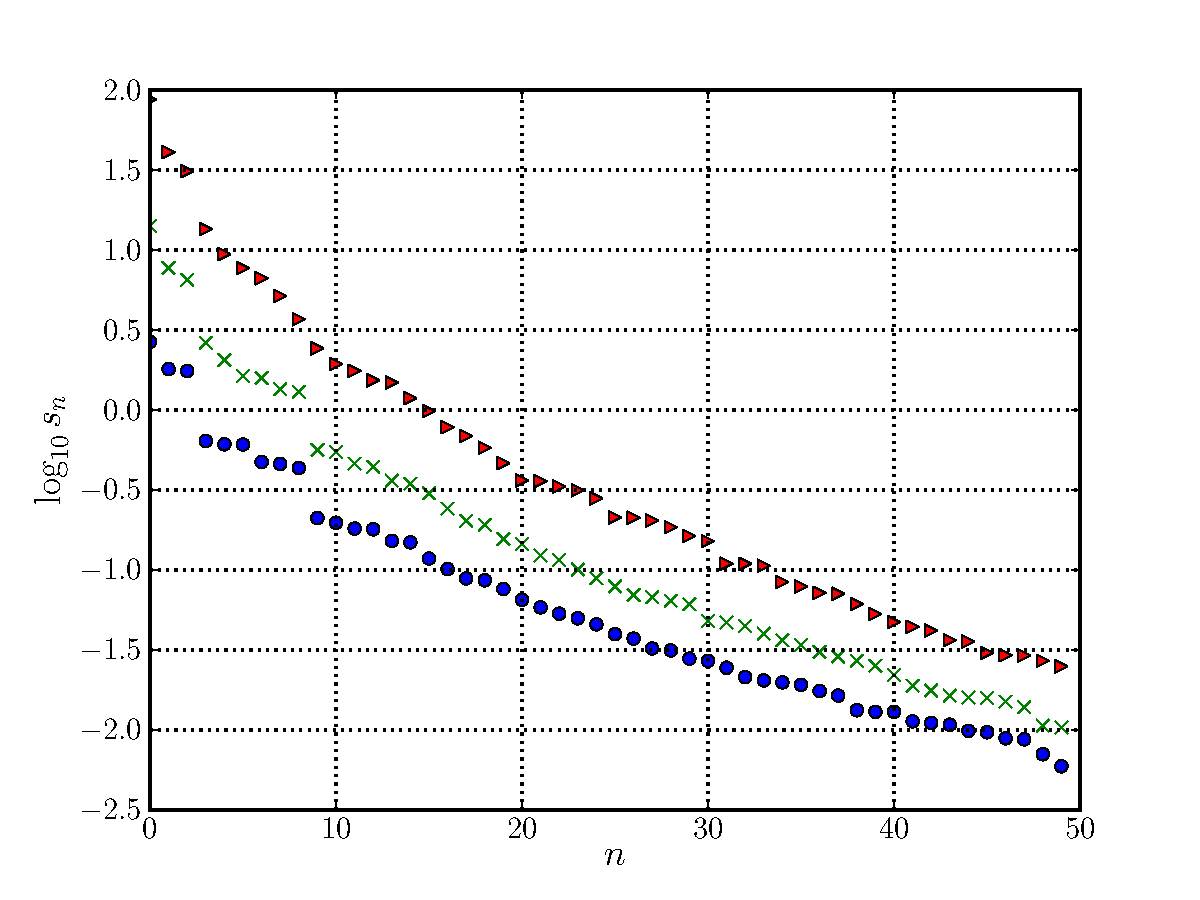
\includegraphics[bb=0in 0in 7.7in 6.3in,width=\StandardFigureWidth,clip]{Images_Methodology/svalues_01.pdf}
	\end{center}	
	\caption{Singular values of the discrete Green's function: $\left(G_h\right)_{xx}$ component (top) and $\left(G_h\right)_{xy}$ component (bottom). 'o' markers are for $N=32$, 'x' markers are for $N=64$, and '$\triangle$' makers are for $N=128$.}
	\label{fig:svalues_00}
\end{figure}

Calculating the SVD of $\ti{G}$ can be expensive. Fortunately, as with the construction of $G_h$, this is a one time cost that can be spread over multiple simulations. However, some care must still be taken as a direct approach to calculating the SVD of $\ti{G}$ would require $O(N^9)$ operations. In Section~\ref{sub:Decomposition} we propose an 
efficient strategy to reduce the cost to $O(pN^3\log N)$ operations.

Finally, turning back to our original optimization problem of minimizing (\ref{meq:L2Dif}), we approximate $A_k(\B{x})$ and $B_k(\B{x})$ at arbitrary positions $\B{x}\in\Omega_{in}$ and $\B{y}\in\Omega_{out}$ by using trilinear interpolation between the surrounding Eulerian grid points. $G_h$ is smooth away from the origin, and its singular vectors are likewise smooth. Trilinear interpolation thus introduces an error of at most $O(h^2)$. For a given interaction between two fiber points we commit this error $p$ times, for a total error on the order of $O(ph^2)$. Assuming $h$ is sufficiently small, this error is smaller than the $O(h)$ error of our expansion and the $O(h)$ error of the IB Method. A numerical verification of the error rate of our expansion is presented below in Section~\ref{Sec:Teecode_Benchmarks}.
\subsection{Decomposition group}
We have seen how to arrive at a decomposition of $G_h$ over a subdomain $\Omega_{in}\times\Omega_{out}$. However, our treecode makes use of $O(N \log N)$ different subdomains. Each subdomain will require a suitable decomposition. Fortunately, we may recycle many of these decompositions for use over multiple subdomains.

Specifically, given two panels $\Panel{P}^1$ and $\Panel{P}^2$ at the same depth in our octree, we may take their expansion coefficient functions to be identical up to translation. That is, given $\B{z}\in\Omega$,
\begin{gather}
A_k^{P_1}(\B{c}^{P_1}+\B{z}) = A_k^{P_2}(\B{c}^{P_2}+\B{z}), \\
B_k^{P_1}(\B{c}^{P_1}+\B{z}) = B_k^{P_2}(\B{c}^{P_2}+\B{z}),
\end{gather}
provided the functions are defined at the points of evaluation. Here, $\B{c}^{P_i}$ denotes the center of panel $P_i$, $i=1,2$.

Due to this equivalence we only need $\log N$ decompositions: one for each level of our octree.
The total precomputational cost of calculating our lookup tables is thus $O(pN^3\log^2 N)$, and the total memory requirement is $O(pN^3\log N)$.




\section{The treecode algorithm}
\label{Sec:TreecodeDetails}
The exposition on the treecode in the previous section was intentionally high level. The intent was to provide an understanding for what a treecode is, why it works, and why it is a good fit for the IB Method. Unfortunately, the details of a treecode implementation are somewhat technical. This section is devoted to providing a more detailed exposition, but is not critical to understanding the thrust of the methods developed in this chapter.

We develop in more detail two components of the treecode algorithm. First, in Section~\ref{sub:octree}, we expand on the algorithms for creating the octree and for using it to evaluate multipole summations. Then, in Section~\ref{sub:Decomposition}, we expand on the algorithm used to arrive at the far field expansions of $G_h$.

\subsection{The octree}
\label{sub:octree}
Note that for this section we adopt a more programmatic syntax, replacing $\Omega_{in}^P$ with $\Panel{P}.\Omega_{in}$, $\B{c}^P$ with $\Panel{P}.\B{c}$, and so on. This is to facilitate the exposition of pseudocode.

We start by defining the notion of a \textit{panel}. A panel is simply a cubic subset of $\Omega$, together with an optional collection of 8 child panels that divide the parent into equal octants. Let $\Panel{P}$ be a panel. To $\Panel{P}$ we associate three vectors, $\Panel{P}.\B{c}, \Panel{P}.\B{a}, \Panel{P}.\B{b} \in\Omega$. $\Panel{P}.\B{a}$ and $\Panel{P}.\B{b}$ serve to define the domain of $\Panel{P}$, given by
\begin{equation}
\Panel{P}.\Omega_{out} = 
[\Panel{P}.\B{a}_0, \Panel{P}.\B{b}_0]\times
[\Panel{P}.\B{a}_1, \Panel{P}.\B{b}_1]\times
[\Panel{P}.\B{a}_2, \Panel{P}.\B{b}_2] \subseteq \Omega.
\end{equation}
The center of $\Panel{P}$ is denoted $\Panel{P}.\B{c} = (\Panel{P}.\B{a} + \Panel{P}.\B{b}) / 2$. This will be the center of expansion for poles inside $\Panel{P}$. We also associate to $\Panel{P}$ a collection of fiber points $\Panel{P}.\B{Y}$ consisting of those points of the fiber configuration $\B{X}$ lying within the domain $\Panel{P}.\Omega_{out}$. The children of $\Panel{P}$, if it has any, are denoted by $\Panel{P}.Child[i]$, for $0\leq i<8$. The children divide $\Panel{P}.\Omega_{out}$ equally, by splitting it into $8$ pieces via the 3 planes $x=\Panel{P}.\B{c}_0$, $y=\Panel{P}.\B{c}_1$, and $z=\Panel{P}.\B{c}_2$.

Given a domain $\Omega = [0,1]^3$, we define an initial panel called $\Panel{Root}$, specified by the bounds $\Panel{Root}.\B{a} = (0,0,0)$ and $\Panel{Root}.\B{b} = (1,1,1)$. We now recursively define child panels, creating the $8$ children of $\Panel{Root}$, then the $8$ children of each of those children, and so on. For a panel $\Panel{P}$ with few fiber points in its domain, say $|\Panel{P}.\B{Y}| < MinPoints$, we truncate the recursive process, leaving $\Panel{P}$ childless. For a pseudocode version of this process, see Function~\ref{func:Create}~CreatePanel. For our simulations we take $MinPoints = 10$. A rigorous accounting of the treecode costs can lead to an optimal value of $MinPoints$, but we did not pursue such an analysis here.

The totality of $\Panel{Root}$ and all of its branches is collectively known as the octree. 
We now introduce the concept of \textit{well separatedness}. Given a point $\B{x}$ and a panel $\Panel{P}$ we say that $\B{x}$ is well separated from $\Panel{P}$ provided that 
\begin{equation}
|\B{x}_i - \Panel{P}.\B{c}_i| \geq 3(\Panel{P}.\B{c}_i - \Panel{P}.\B{a}_i), \qquad\text{for $i=0,1,2$}, \label{ws}
\end{equation}
that is, provided that $\B{x}$ is sufficiently far from the center of $\Panel{P}$. We now consider the pair of subsets $(\Panel{P}.\Omega_{in}, \Panel{P}.\Omega_{out})$, where $\Panel{P}.\Omega_{in}$ is the collection of points in $\Omega$ that are well separated from $\Panel{P}$. We assume that we can expand $G_h$ over $\Panel{P}.\Omega_{in}\times\Panel{P}.\Omega_{out}$, arriving at two collections of coefficient functions $\{\Panel{P}.A_k\}_{k=1}^p$ and $\{\Panel{P}.B_k\}_{k=1}^p$. In addition,  we define
\begin{equation}
\Panel{P}.B_{out} = \{i\in B | \B{X}_i\in\Panel{P}.\B{Y}\},
\end{equation}
as the collection of indices associated with fiber points in $\Panel{P}.\B{Y}$. 

Suppose now that we are given a fiber force $\B{F}$ and wish to evaluate its influence at points $\B{x}$ in the fluid domain. For each $\B{x}$ this influence is given by
\begin{equation}
\sum_{1\leq j\leq N_B} G_h(\B{x} - \B{X}_j) \B{F}_j.
\end{equation}
To evaluate this efficiently, we first loop over each panel $\Panel{P}$ and calculate the far field expansion of all the poles located in $\Panel{P}.\Omega_{out}$. The $k$-th term of this expansion is given by
\begin{equation}
\Panel{P}.H_k \equiv \sum_{j\in \Panel{P}.B_{out}}
\Panel{P}.B_k(\B{X}_j) \tilde{F}_j.
\label{meq:OutgoingA}
\end{equation}
If $\B{x}$ is well separated from $\Panel{P}$, then the incoming effect on $\B{x}$ from $\Panel{P}$ is given by
\begin{equation}
\B{E}^T \full\sum_{k=1}^{p}\Panel{P}.A_k(\B{X}_i)\Panel{P}.H_k.
\label{meq:IncomingA}
\end{equation}
We can now evaluate the entire influence of $\B{F}$ on a point $\B{x}$. The process is best described in recursive form. A pseudocode is presented in Function~\ref{func:Eval}~Evaluate. 

Because our treecode must be invoked multiple times per timestep, it is critical to streamline its evaluation. There are two key points to keep in mind. First, calculations of the expansion coefficients can be recycled. In Section~\ref{Sec:Treecode_Expansions} we will detail the form of the coefficient functions $A_k$ and $B_k$. Each evaluation requires an expensive trilinear interpolation. Avoiding duplications of these calculations provides substantial speedup. Second, using the treecode to evaluate the influence at a particular point $\B{x}$ requires traversing the octree. This traversal can be stored as a template so that additional evaluations at $\B{x}$ do not require a recursive call.

There are thus two different function calls: the actual evaluation function, which takes in a fiber force $\B{F}$ and returns the influence over the entire structure $\B{X}$; and a pre-evaluation function, which does a variety of computations used to streamline the evaluation function. The cost of the pre-evaluation function is much higher than that of the evaluation function itself. However, the pre-evaluation function is called only once per timestep.

We mention one further implementation detail regarding the treatment of the domain $\Panel{P}.\Omega_{in}$ for a given panel $\Panel{P}$. Rather than treating this is as a single domain,  we break it into eight equally sized pieces, corresponding to the eight octants around the panel's center $\Panel{P}.\B{c}$. For each piece we must then have separate collections of coefficient functions $\{\Panel{P}.A_k\}_{k=1}^{p}$, $\{\Panel{P}.B_k\}_{k=1}^{p}$, as well as a separate expansion $\{\Panel{P}.H_k\}_{k=1}^{p}$.

This additional detail may seem costly at first, but in fact it increases the speed of the treecode substantially. By restricting our attention to a smaller domain it is possible to find expansions which converge much more rapidly.

\begin{algorithm}
\caption{CreatePanel$(\B{a}, \B{b})$}
\label{func:Create}
\begin{algorithmic}
\STATE $\Panel{P} \gets \B{new} \, Panel$
\STATE $\Panel{P}.\B{a} = \B{a}$
\STATE $\Panel{P}.\B{b} = \B{b}$
\STATE $\Panel{P}.\B{c} = (\B{a} + \B{b}) / 2$
\IF {$\Panel{P}.Parent$ exists}
	\STATE $\Panel{P}.\B{Y} = \Panel{P}.Parent.\B{Y} \cap \Panel{P}.\Omega_{out}$
\ELSE
	\STATE $\Panel{P}.\B{Y} = \B{X}^n \cap \Panel{P}.\Omega_{out}$
\ENDIF
\IF {$|\Panel{P}.\B{Y}| > MinPoints$}
	\STATE $ \Panel{P}.Child[0] = \text{CreatePanel}(
	\Panel{P}.\B{a},
	\Panel{P}.\B{c})$
	\STATE $ \Panel{P}.Child[1] = \text{CreatePanel}(
	[\Panel{P}.\B{c}_0, \Panel{P}.\B{a}_1, \Panel{P}.\B{a}_2] ,
	[\Panel{P}.\B{b}_0, \Panel{P}.\B{c}_1, \Panel{P}.\B{c}_2] )$
	\STATE $ \Panel{P}.Child[2] = \text{CreatePanel}(
	[\Panel{P}.\B{a}_0, \Panel{P}.\B{c}_1, \Panel{P}.\B{a}_2] ,
	[\Panel{P}.\B{c}_0, \Panel{P}.\B{b}_1, \Panel{P}.\B{c}_2] )$
	\STATE $ \Panel{P}.Child[3] = \text{CreatePanel}(
	[\Panel{P}.\B{c}_0, \Panel{P}.\B{c}_1, \Panel{P}.\B{a}_2] ,
	[\Panel{P}.\B{b}_0, \Panel{P}.\B{b}_1, \Panel{P}.\B{c}_2] )$
	\STATE $ \Panel{P}.Child[4] = \text{CreatePanel}(
	[\Panel{P}.\B{a}_0, \Panel{P}.\B{a}_1, \Panel{P}.\B{c}_2] ,
	[\Panel{P}.\B{c}_0, \Panel{P}.\B{c}_1, \Panel{P}.\B{b}_2] )$
	\STATE $ \Panel{P}.Child[5] = \text{CreatePanel}(
	[\Panel{P}.\B{c}_0, \Panel{P}.\B{a}_1, \Panel{P}.\B{c}_2] ,
	[\Panel{P}.\B{b}_0, \Panel{P}.\B{c}_1, \Panel{P}.\B{b}_2] )$
	\STATE $ \Panel{P}.Child[6] = \text{CreatePanel}(
	[\Panel{P}.\B{a}_0, \Panel{P}.\B{c}_1, \Panel{P}.\B{c}_2] ,
	[\Panel{P}.\B{c}_0, \Panel{P}.\B{b}_1, \Panel{P}.\B{b}_2] )$
	\STATE $ \Panel{P}.Child[7] = \text{CreatePanel}(
	\Panel{P}.\B{c},
	\Panel{P}.\B{b})$
\ENDIF
\RETURN $\Panel{P}$
\end{algorithmic}
\end{algorithm}

\begin{algorithm}
\caption{Evaluate$(\B{x}, \Panel{P})$}
\label{func:Eval}
\begin{algorithmic}
\IF [$\B{x}$ is well separated from $\Panel{P}$] {$\B{x} \in \Panel{P}.\Omega_{in}$}
	\RETURN $\B{E}^T \full\sum_{k=1}^{p}\Panel{P}.A_k(\B{X}_i)\Panel{P}.H_k$
\ELSE
	\IF {$\Panel{P}$ has children}
		\STATE $S = 0$ \COMMENT{the $3\times 3$ zero tensor}
		\FOR {$i = 0$ to $7$}
			\STATE $S = S + \text{Evaluate}(\B{x}, \Panel{P}.Child[i])$
		\ENDFOR
		\RETURN S
	\ELSE[do a direct summation]
		\RETURN $\full\sum_{j\in \Panel{P}.B_{out}} G_h(\B{x}, \B{X}_j) \B{F}_j$
	\ENDIF
\ENDIF
\end{algorithmic}
\end{algorithm}

\subsection{Far field expansions: calculating a truncated SVD of restrictions of $G_h$}
\label{sub:Decomposition}
The far field expansions of $G_h$ that we employ are known as rank-1 decompositions, and can be obtained via the Singular Value Decomposition. Note that when we decompose $G_h$ we consider it properly as a function defined on $\Omega \times \Omega$, not as a field over $\Omega$. For actual evaluations of $G_h$, however, we still assume translation invariance, treating $G_h$ as a field and making use of our lookup table on $\C{G}_h$.

Treating $G_h$ as a function defined only on $\C{G}_h\times \C{G}_h$, we may write $G_h$ as an $N^3\times N^3$ matrix and seek its SVD. Typical SVD algorithms would require $O(N^9)$ operations. This is too great a cost, even for a precomputation. The two key ingredients for accelerating the computation of the SVD are, first, that we only require the first $p$ singular values of $G_h$, not all $N^3$ of them, and, second, that our approximation to $G_h$ is convolutional. We present an algorithm that takes advantage of these ingredients. While matrices are convenient for relating to the SVD, in what follows we treat $G_h$ directly as a function, and abandon any use of matrices.

We will focus on the discretized domain $\C{G}_h$ and a particular pair of subsets, $\left(\Omega_{in}, \Omega_{out}\right)$, over which we wish to decompose $G_h$. We will require a few definitions.
Given two functions $f$ and $g$ defined over $\Omega_{in}\cap\C{G}_h$ and $\Omega_{out}\cap\C{G}_h$ respectively, we define the outer product $f\otimes g$ via the relation
\begin{equation}
\left(f\otimes g\right)(\B{x},\B{y}) = f(\B{x})g(\B{y}),
\end{equation}
for $\B{x}\in\Omega_{in}\cap\C{G}_h$, $\B{y}\in\Omega_{out}\cap\C{G}_h$. If $f'$ is another function defined over $\Omega_{in}\cap\C{G}_h$, and both $f$ and $f'$ are $3\times 3$ tensor fields, then we define the componentwise inner product $\LL f, f' \RR$ to be a $3\times 3$ tensor given by
\begin{equation}
\LL f, f' \RR_{ij} = \sum f_{ij}(\B{x})f'_{ij}(\B{x}), 
\end{equation}
where the sum is taken over all $\B{x}\in\Omega_{in}\cap\C{G}_h$.

For a scalar function $f$ defined on $\C{G}_h$, the $L^2$ norm is given by
\begin{equation}
\norm{f}_2^2 = \sum_{\B{x}\in\C{G}_h} f(\B{x})^2.
\end{equation}
For functions with other domains the norm is implicitly taken over the entire domain of the function.
For a $3\times 3$ tensor valued function $g$ on $\C{G}_h$, we define $\norm{g}_2$ to be a $3\times 3$ tensor given by $\left(\norm{g}_2\right)_{ij} = \norm{g_{ij}}_2$. 

Now, we are seeking a collection of $2p$ functions, $\{A_k\}_{k=1}^p$ and $\{B_k\}_{k=1}^p$, each a $3\times 3$ tensor field over $\C{G}_h$, such that the rank-1 decomposition
\begin{equation}
\sum_{k=1}^{p} A_k \otimes B_k
\end{equation}
is as close as possible to $G_h$ in the $L^2$ sense. From SVD theory we know that given this truncated decomposition we will have simultaneously minimized 
\begin{equation}
\norm{G_h - \sum_{k = 1}^q A_k \otimes B_k}_2
\label{meq:ReducedMin}
\end{equation}
for any $q$ such that $1\leq q \leq p$, where the norm is taken over the domain $\Omega_{in}\cap\C{G}_h\times\Omega_{out}\cap\C{G}_h$. We may take advantage of this result by first finding $A_1$ and $B_1$ such that (\ref{meq:ReducedMin}) is minimized for $q=1$. Next, we can hold $A_1$ and $B_1$ fixed as we seek the $A_2$ and $B_2$ that minimize (\ref{meq:ReducedMin}) for $q=2$. Assuming we have iterated this procedure up to $q = l-1$, we detail the procedure for finding $A_l$ and $B_l$.

First, $A_l$ and $B_l$ are exactly the tensor fields that minimize
\begin{equation}
L\equiv \norm{G_h - \sum_{k = 1}^{l} A_k\otimes B_k}_2^2 = \norm{G_h' - A_l\otimes B_l}_2^2,
\label{meq:l_Min}
\end{equation}
where
\begin{equation}
G_h'\equiv G_h - \sum_{k = 1}^{l-1} A_k\otimes B_k.
\end{equation}
If we fix $B_l$ then we can minimize $L$ in (\ref{meq:l_Min}) by the method of least squares.  We fix a $\B{z}$ in $\Omega_{in}$ and derive $L$ with respect to $A_l(\B{z})$, obtaining
\begin{align}
-\frac{1}{2} \frac{\partial L}{\partial A_l(\B{z})}
&=
-\frac{1}{2} \frac{\partial}{\partial A_l(\B{z})} \sum \left(G_h'(\B{x},\B{y}) - A_l(\B{x})B_l(\B{y})\right)^2,
\end{align}
where the sum is taken over $\B{x}\in\Omega_{in}\cap\C{G}_h,\B{y}\in\Omega_{out}\cap\C{G}_h$. Dropping the terms independent of  $A_l(\B{z})$ leaves
\begin{align}
&
\sum \left(G_h'(\B{z},\B{y}) - A_l(\B{z})B_l(\B{y})\right)B_l(\B{y}) \nonumber \\
&=
\left[ \sum G_h'(\B{z},\B{y})B_l(\B{y}) \right] - A_l(\B{z})\norm{B_l}_2^2,
\label{meq:ConvolutionalSum}
\end{align}
where the sum is now over $\B{y}\in\Omega_{out}\cap\C{G}_h$. The sum in (\ref{meq:ConvolutionalSum}) is  nearly a convolution. We seek to recast it as such.

First, we define the indicator functions
\begin{equation}
\B{\B{I}}_{in}(\B{x}) = \begin{cases}
1 \qquad &\text{if $\B{x} \in \Omega_{in}\cap\C{G}_h$} \\
0 \qquad &\text{otherwise}, \end{cases}
\end{equation}
and
\begin{equation}
\B{\B{I}}_{out}(\B{x}) = \begin{cases}
1 \qquad &\text{if $\B{x} \in \Omega_{out}\cap\C{G}_h$} \\
0 \qquad &\text{otherwise}. \end{cases}
\end{equation}
$A_l$ is a field over $\Omega_{in}\cap\C{G}_h$, but we may identify $A_l\B{\B{I}}_{in}$ with a field defined over all of $\C{G}_h$ in the natural way. We may likewise identify $B_l\B{\B{I}}_{out}$ with a field defined over all of $\C{G}_h$. These identifications allow us to express the sum in (\ref{meq:ConvolutionalSum}) as a convolution against $G_h$ over all of $\C{G}_h$, minus some correction.
\begin{align}
&\left[ \sum G_h'(\B{z},\B{y})B_l(\B{y}) \right] \nonumber \\
&= 
\left[ \sum G_h(\B{z} - \B{y})B_l(\B{y}) \right] -
\sum_{k = 1}^{l-1} \sum A_k(\B{z}) B_k(\B{y}) B_l(\B{y}) \\
&=
\left[(G_h*(B_l\B{I}_{out}))\B{I}_{in}\right](\B{z}) -
\sum_{k = 1}^{l-1} A_k(\B{z}) \LL B_k, B_l \RR. \nonumber
\end{align}
Requiring that the derivatives of $L$ be zero in (\ref{meq:ConvolutionalSum}), we solve for $A_l$ as
\begin{equation}
A_l = \frac{1}{\norm{B_l}_2^2}
\left[
(G_h*(B_l\B{I}_{out}))\B{I}_{in}
- \sum_{k = 1}^{l-1} A_k \LL B_k, B_l \RR
\right].
\label{meq:SolveForA}
\end{equation}
If we fix $A_l$ we can solve the equivalent least squares problem for $B_l$, obtaining
\begin{equation}
B_l = \frac{1}{\norm{A_l}_2^2}
\left[
(G_h*(A_l\B{I}_{in}))\B{I}_{out}
- \sum_{k = 1}^{l-1} B_k \LL A_k, A_l \RR
\right].
\label{meq:SolveForB}
\end{equation}
Equations (\ref{meq:SolveForA}) and (\ref{meq:SolveForB}) must be solved simultaneously. We approximate the solution to this system via the iterative method
\begin{equation}
\left\{
\begin{aligned}
A_l^{n+1} = \frac{1}{\norm{B_l^n}_2^2}
&\left[
(G_h*(B_l^n\B{I}_{out}))\B{I}_{in}
- \sum_{k = 1}^{l-1} A_k \LL B_k, B_l^n \RR
\right], \\
B_l^{n+1} = \frac{1}{\norm{A_l^{n+1}}_2^2}
&\left[
(G_h*(A_l^{n+1}\B{I}_{in}))\B{I}_{out}
- \sum_{k = 1}^{l-1} B_k \LL A_k, A_l^n \RR
\right].
\label{meq:PowerMethod}
\end{aligned}
\right.
\end{equation}
We require an initial guess for this iteration, call it $B_l^0$, with the restriction that $B_l^0$ not be a linear combination of $\{B_k\}_1^{l-1}$.

(\ref{meq:PowerMethod}) is a type of power method. Power methods are known to converge quickly provided the singular values of $G_h$ are sufficiently separated. For our particular problem (\ref{meq:PowerMethod}) converges in $20$ to $30$ iterations. A stopping criteria can be improvised based on $\norm{B_l^{n+1} - B_l^n}$, but for simplicity we simply fix the number of iterations at 30.

We have written (\ref{meq:PowerMethod}) in a form that allows for a minimum of computational effort. The convolutions against $G_h$ may be efficiently computed in discrete Fourier space at an $O(N^3\log N)$ cost, while the inner products require only $O(N^3)$ operations each. Thus, the total cost per iteration of (\ref{meq:PowerMethod}) is $O(N^3\log N)$. We require $O(\log N)$ decompositions, hence the total precomputational cost is $O(30pN^3\log^2 N)$.


\section{Treecode benchmarks}
\label{Sec:Teecode_Benchmarks}
In this section we present a numerical validation and performance evaluation of the treecode. To this end, we use a test problem which consists of 
an immersed, flat plate with fiber points $\B{X}_i$ tethered to fixed points $\B{T}$ and with a fiber force  $\C{A}_{h_B}(\B{X}) = \sigma(\B{T} - \B{X})$ (see Section~\ref{sub:plate} for details on this problem setup).  We fix $N=128$, $\sigma=10^7$, $\Delta t=0.002$,  and vary $N_B$ and $p$.

 The performance of the treecode is analyzed through the performance of two different function calls: the evaluation function, which takes in a fiber force $\B{F}$ and returns the influence at every fiber point $\B{X}$; and a pre-evaluation function, which does a variety of computations used to streamline the evaluation function. The pre-evaluation function is called only once per timestep

We examine accuracy first. There are two confounding factors that degrade the accuracy of our treecode. The first is that we approximate $G_h$ as a truncated rank-1 decomposition. The second is that we introduce error into the simulation by assuming translation invariance of $G_h$. In order to analyze the first component separately we consider an immersed plate where the fiber points lie exactly on Eulerian intersection. This avoids the introduction of any error from translation.

We calculate the error according to the following procedure. We first make an $O(h)$ perturbation of the fiber $\B{X}$. This perturbation generates a force $\B{F}$ on the fiber. We then evaluate $\C{M}_n\B{F}$ using both the treecode and a direct fluid solve and take the sup norm of the difference.

The blue line in Figure~\ref{fig:Benchmark_p_MaxDif} shows the resulting decrease in error for increasing values of $p$. If we do not restrict the fiber points to Eulerian intersections then the above procedure returns a different decay line, seen as the green line in Figure~\ref{fig:Benchmark_p_MaxDif}. Note that past $p=10$ no additional reduction in error is achieved. This is the point at which the $O(h)$ error from our approximation to $G_h$ overwhelms the error introduced by using a truncated expansion. In actual simulations fiber points can not be restricted to Eulerian intersections, hence any value of $p > 10$ would be computationally wasteful.


If we fix $p=10$ and compute the error for various values of $h$ we see that it does indeed decrease at least as fast as $O(h)$, as seen in Figure~\ref{fig:Benchmark_h_MaxDif}, consistent with the error bounds presented in Section~\ref{sub:TranslationError_2D} and Section~\ref{sub:TranslationError_3D}.


\begin{figure}[!b]
	\begin{center}
		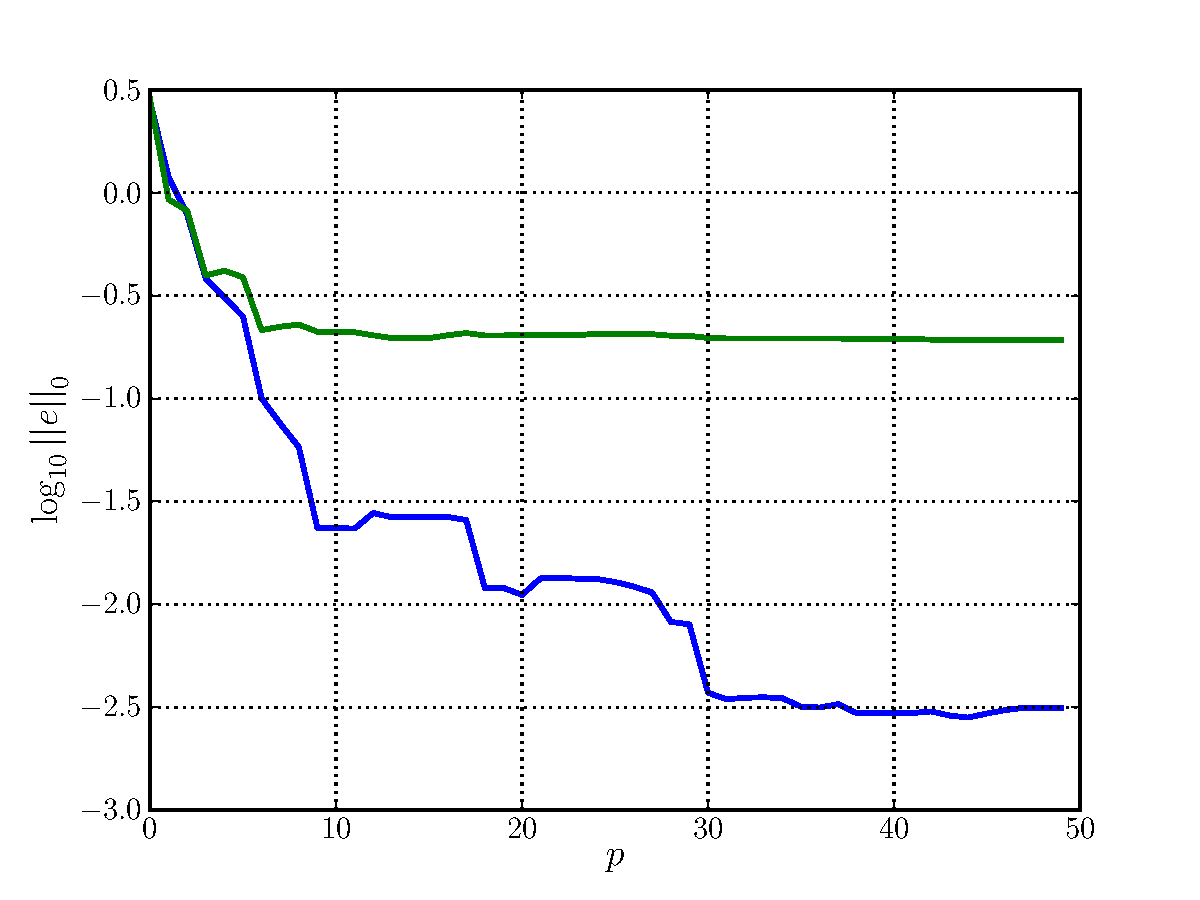
\includegraphics[bb=0in 0in 7.7in 6.3in,width=\StandardFigureWidth,clip]{Images_Methodology/Benchmark_p_MaxDif.pdf}
	\end{center}
	\caption{Log of the sup norm of the difference between $\C{M}_n\B{F}$ calculated via a fluid solve and via the treecode for various values of $p$, where $p$ is the number of terms in the treecode's far field expansion. $N=128$ and $N_B=N^2/4$. The blue line is for a plate with fiber points aligned to the Eulerian grid. The green line is for a plate with no restrictions on the fiber point locations.}
	\label{fig:Benchmark_p_MaxDif}
\end{figure}

\begin{figure}[!b]
	\begin{center}
		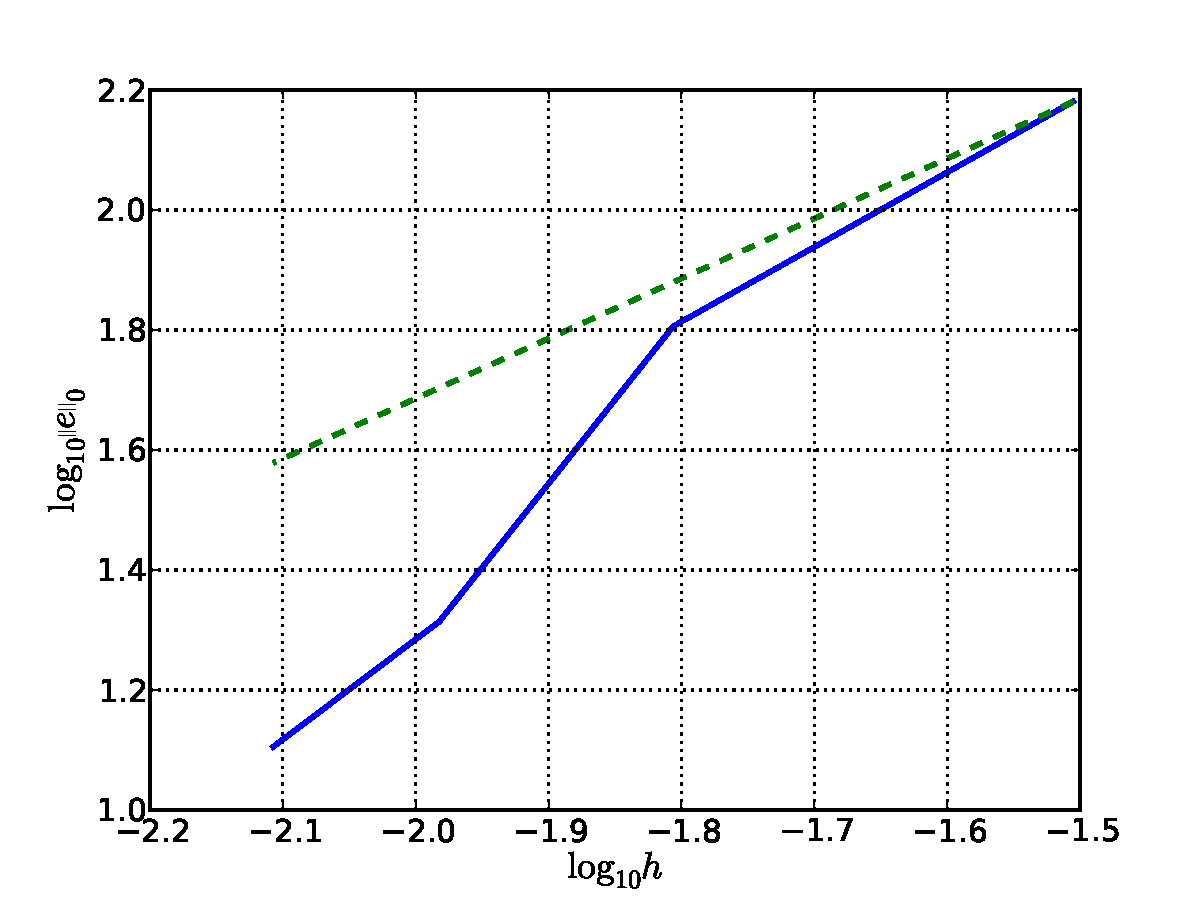
\includegraphics[bb=0in 0in 7.7in 6.3in,width=\StandardFigureWidth,clip]{Images_Methodology/Benchmark_h_MaxDif.pdf}
	\end{center}
	\caption{Log of the sup norm of the difference between $\C{M}_n\B{F}$ calculated via a fluid solve and via the treecode for various values of $h$, with $p=10$. The solid blue line is the error. The dashed green line is a reference line with slope $1$.}
	\label{fig:Benchmark_h_MaxDif}
\end{figure}

We now analyze the performance of the treecode. All units of time are given as multiples of the average time to perform a fluid solve with $N=128$.
We first fix $p=10$ and vary $N_B$. The resulting CPU time for the evaluation of $\C{M}_n\B{F}$ for an arbitrary $\B{F}$ is shown in Figure~\ref{fig:Benchmark_Nb_EvalTime}. The corresponding CPU time for the pre-evaluation call is given in Figure~\ref{fig:Benchmark_Nb_PreEvalTime}. Both scale nearly linearly in $N_B$,  as expected.



\begin{figure}[!b]
	\begin{center}
		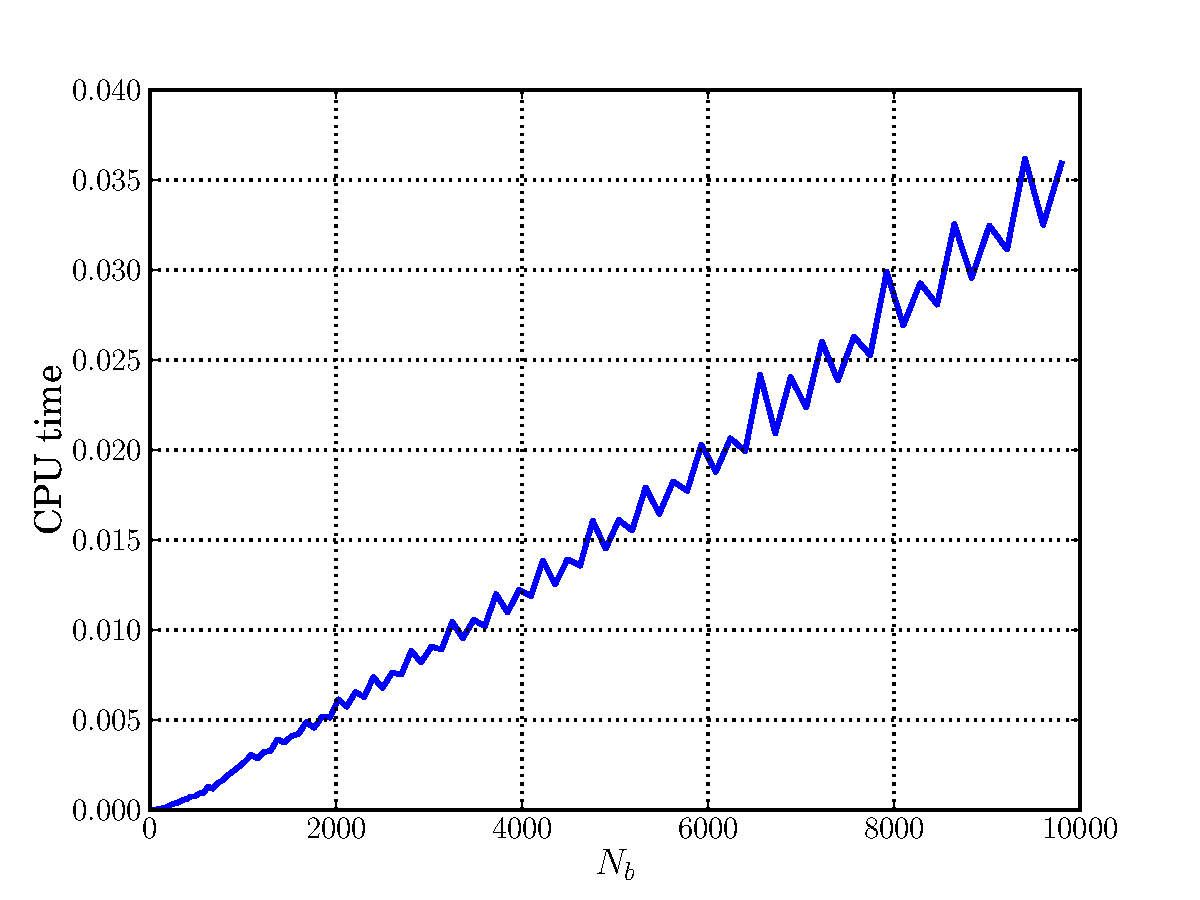
\includegraphics[bb=0in 0in 7.7in 6.3in,width=\StandardFigureWidth,clip]{Images_Methodology/Benchmark_Nb_EvalTime.pdf}
	\end{center}
	\caption{CPU time for the evaluation of $\C{M}_n\B{F}$ via the treecode for increasing values of $N_B$, where $p=10$. Time is given as multiples of the average time to perform a fluid solve, for $N=128$.}
	\label{fig:Benchmark_Nb_EvalTime}
\end{figure}

\begin{figure}[!b]
	\begin{center}
		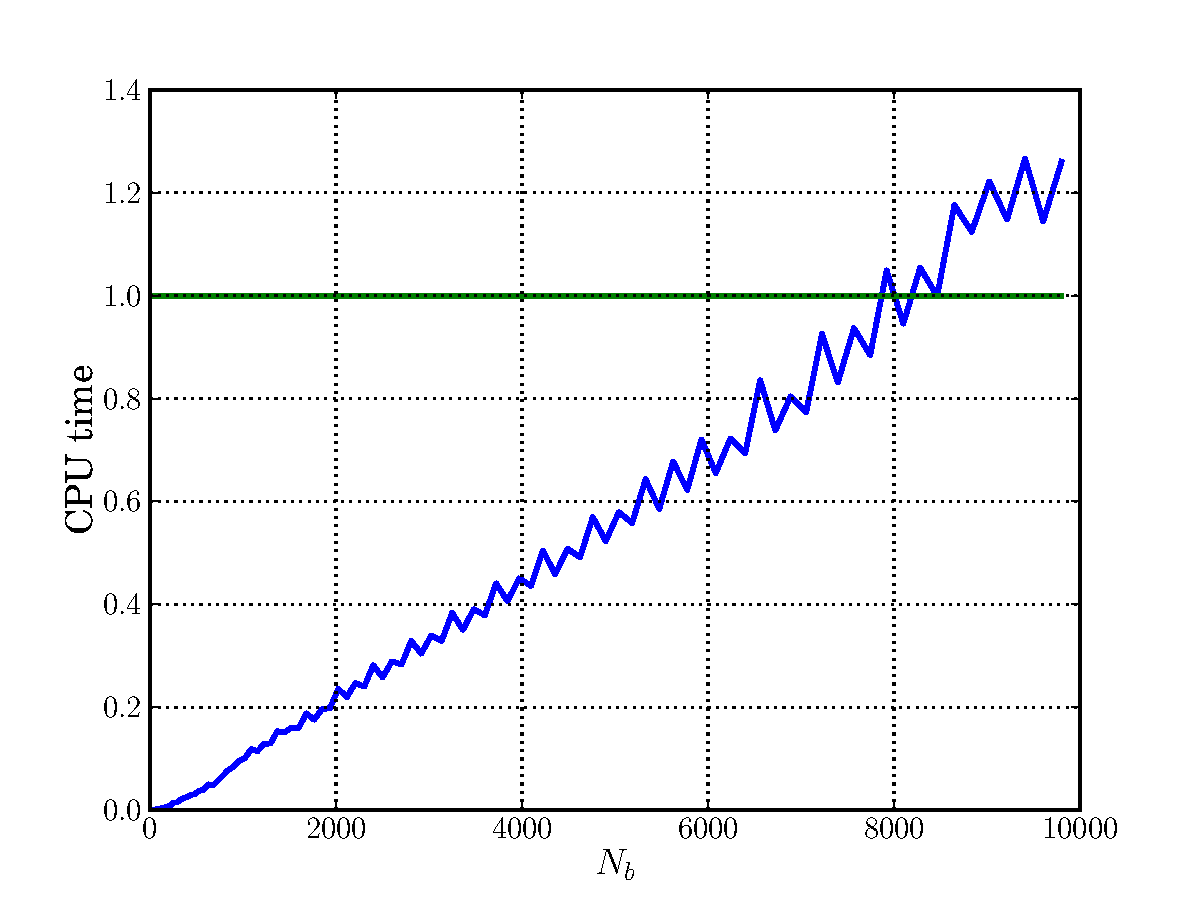
\includegraphics[bb=0in 0in 7.7in 6.3in,width=\StandardFigureWidth,clip]{Images_Methodology/Benchmark_Nb_PreEvalTime.pdf}
	\end{center}
	\caption{CPU time for the treecode pre-evaluation for increasing values of $N_B$, where $p=10$. Time is given as multiples of the average time to perform a fluid solve, for $N=128$. The green line represents the cost of one fluid solve.}
	\label{fig:Benchmark_Nb_PreEvalTime}
\end{figure}

\Comment{ % Extra tables, showing the cost of the treecode for increasing $p$
\begin{figure}[!b]
	\begin{center}
		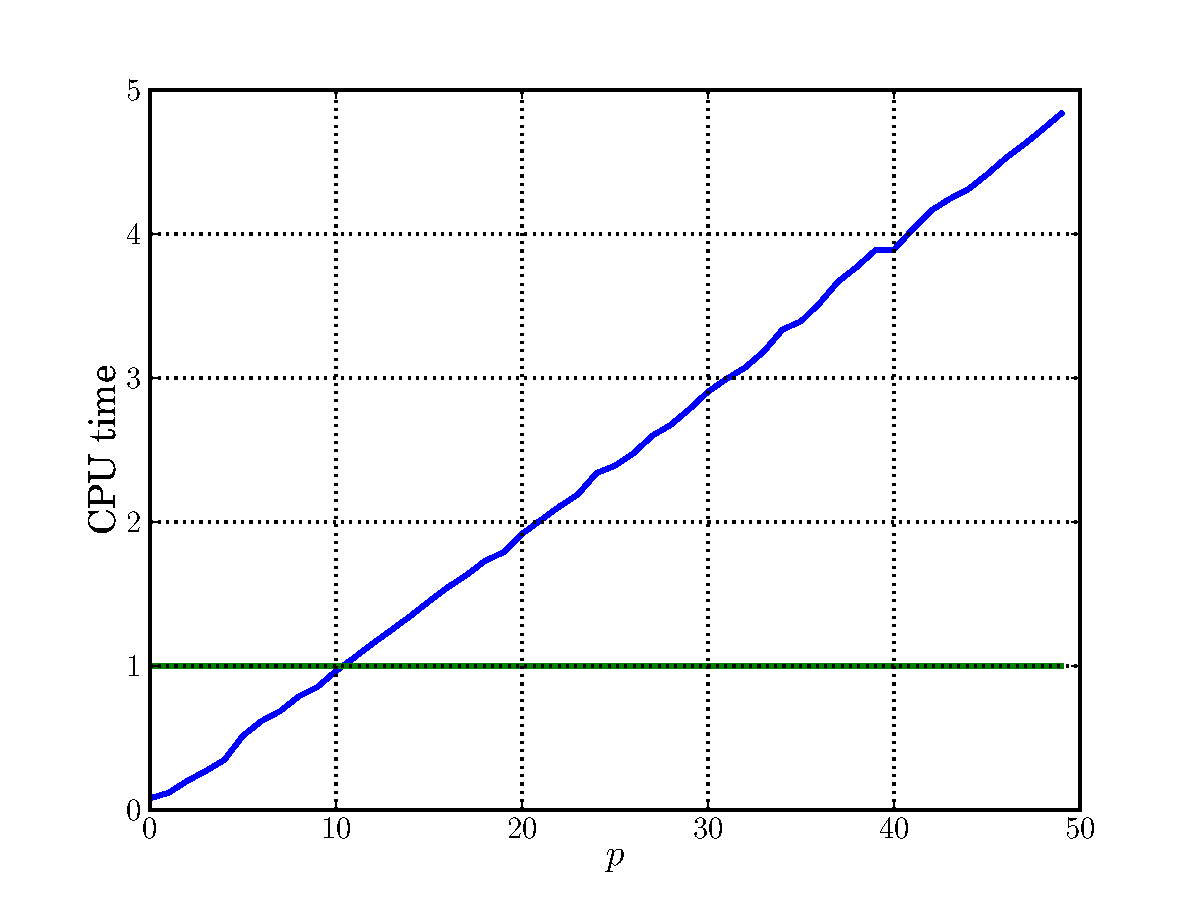
\includegraphics[bb=0in 0in 7.7in 6.3in,width=\StandardFigureWidth,clip]{Images_Methodology/Benchmark_p_PreEvalTime.pdf}
	\end{center}
	\caption{CPU time for the treecode pre-evaluation for increasing values of $p$, where $N_B=N^2/2$, $N=128$. Time is given as multiples of the average time to perform a fluid solve. The green line represents the cost of one fluid solve.}
	\label{fig:Benchmark_p_PreEvalTime}
\end{figure}

\begin{figure}[!b]
	\begin{center}
		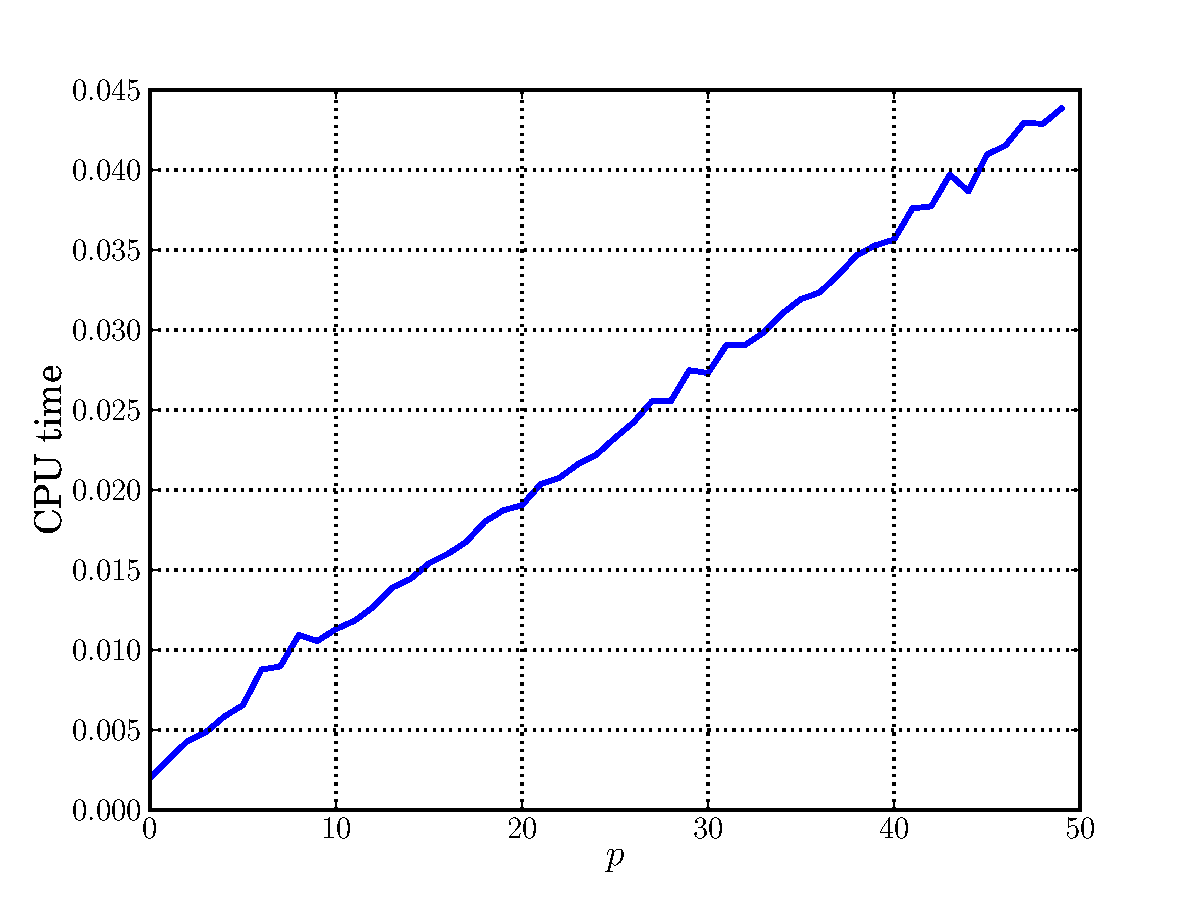
\includegraphics[bb=0in 0in 7.7in 6.3in,width=\StandardFigureWidth,clip]{Images_Methodology/Benchmark_p_EvalTime.pdf}
	\end{center}
	\caption{CPU time for the evaluation of $\C{M}_n$ via the treecode for increasing values of $p$, where $N_B=N^2/2$, $N=128$. Time is given as multiples of the average time to perform a fluid solve.}
	\label{fig:Benchmark_p_EvalTime}
\end{figure}
}


Most analytic expansions used for treecodes and FMM codes, including Taylor series expansions, are not optimal, in the sense that a different expansion would yield higher accuracy for the same number of terms. We approximate directly the $L_2$-optimal expansion. We note that the extension of treecodes and FMM codes to generic kernels, and the associated use of the SVD decomposition in particular, has been studied since the early 90s, see e.g.~\cite{SVDFMM_GimbutasEtAl} for a more detailed exposition.


\section{Krylov Methods}
\label{sec:KrylovMethods}
The treecode method can be easily adapted to compute Gauss-Seidel iterations for the implicit system (\ref{meq:Xnl}). In this sense the treecode is a generalization of the matrix method: it allows for all the iterative methods that the matrix method allows for, while providing additional speedups, especially in the 3D case. In particular we can use the treecode to implement a multigrid solver.

Importantly, however, for many applications evaluation of terms of the form $\C{M}_n\B{F}$ via the treecode is so efficient that sophisticated solvers such as multigrid are not necessary. In this section we present two applications of the treecode in 3D. The iterative method employed is a simple conjugate gradient. We will see, however, that solving (\ref{meq:Xnl}) is nonetheless very cheap, amounting to a fraction of the total cost of an implicit timestep.


\subsection{Case III: An immersed plate.}
\label{sub:plate}
For the first test of our proposed methodology we simulate flow past an immersed plate. The plate is a flat square of dimensions $1/2$ by $1/2$ and is discretized as an $(M+1)\times (M+1)$ grid of fiber points, where $M = \floor{N\sqrt{2}/2}$. This yields $N_B=529$, 2116, and 8281 for $N=32$, 64, and 128 respectively.

For each $j,k$ such that $0 \leq j \leq M, 0 \leq k \leq M$ we have a fiber point $\B{X}_{j,k}\in\Omega$. Each fiber point $\B{X}_{j,k}$ is tethered to a corresponding fixed point $\B{T}_{j,k}\in\Omega$ given by
\begin{equation}
\B{T}_{j,k}= (0.25,0.25,0.5) + \frac{1}{2M} (j, k, 0).
\end{equation}
The tethers induce a force $\C{A}_{h_B}(\B{X}) = \sigma(\B{T} - \B{X})$ which acts to restore the plate to equilibrium, as well as to bind the plate against the fluid flow pushing against it. The initial configuration of the plate is taken to be the equilibrium state $\B{X}^0 = \B{T}$. Note that, among non-empty Eulerian grid cells, the average number of fiber points per cell is roughly $2$. This is the minimum density needed to prevent unreasonable spurious currents across the plate.

A fluid flow is induced by adding a time dependent forcing vector $\B{f}(t)$ to the right hand side of (\ref{meq:dmoment}). We take $\B{f}(t) = 100 (0, \sin \theta(t), \cos \theta(t))$, where $\theta(t) = 4\cos(6\pi t / T) / \pi$ and $T=0.25$ is the total simulation time. The addition of $\B{f}(t)$ alters the explicit term $\B{b}^n$ in our implicit system to
\begin{equation}
\B{b}^n = \B{X}^n + \Delta t \C{S}^*_n \C{L}_h [\B{u}^n-\Delta t \B{u}^n \cdot \nabla_h \B{u}^n + \Delta t \B{f}(t^n)].
\label{meq:bn_flow}
\end{equation}
The induced flow has a Reynolds number of about 10.

$\C{A}_{h_B}$ is affine, not linear, thus we cannot directly apply CG to solve the implicit system. Suppose we denote our initial guess for $\B{X}^{n+1}$ as $\B{X}^{n+1,0}$. We define $\bar{\B{X}}^{n+1} = \B{X}^{n+1}-\B{X}^{n+1,0}$ and recast our implicit system in terms of $\bar{\B{X}}^{n+1}$. We define $\C{A}'_{h_B}(\B{X}) = -\sigma\B{X}$ and  a new explicit term
\begin{equation}
\bar{\B{b}}^n = \B{X}^n - \B{X}^{n+1,0} + \Delta t \C{S}^*_n \C{L}_h [\B{u}^n-\Delta t \B{u}^n \cdot \nabla_h \B{u}^n + \C{A}_{h_B}(\B{X}^{n+1,0}) + \Delta t \B{f}(t^n)].
\label{meq:bn_change}
\end{equation}
Our implicit system then becomes
\begin{equation}
\bar{\B{X}}^{n+1} = \C{M}_n\C{A}'_{h_B} (\bar{\B{X}}^{n+1}) + \bar{\B{b}}^n.
\label{meq:ImplicitChange}
\end{equation}
Here $\C{A}'_{h_B}$ is linear negative definite, thus $I - \C{M}_n\C{A}'_{h_B}$ is positive definite and we can solve (\ref{meq:ImplicitChange}) via CG.
For the CG we use a convergence tolerance of $0.0001$, which is at least $10$ times smaller than the error of the method. For an initial guess we take $\B{X}^{n+1,0}=\B{X}^n$.

We perform both explicit and implicit simulations for $N=32,64,128$ and various values of $\sigma$. 
The explicit simulation uses a standard Forward Euler/Backward Euler  (FE/BE) discretization, i.e. implicit in the viscous term but explicit in all the other terms, including the tension force. The largest stable timestep is given by the empirical formula $\Delta t = 10h\sigma^{-1/2}$.
 Table~\ref{table:ExplicitTimestep_Plate}  provides a list of the values of $\Delta t$ required for a stable simulation using the FE/BE discretization.
 Note that even for modest resolutions the timestep is prohibitively small.
\begin{table}
\caption{ $\Delta t$ in the explicit simulations of the immersed plate for various values of $N$ and $\sigma$. $\Delta t$ is approximately the largest {\em stable} timestep, given by the formula $\Delta t =10h\sigma^{-1/2}$.}
\label{table:ExplicitTimestep_Plate}
\begin{center}

\begin{tabular}{c c c c c c}
  &  $\sigma=10^7$ & $\sigma=10^8$ & $\sigma=10^9$ & $\sigma=10^{10}$ & $\sigma=10^{11}$ \\
\cline{2-6}
\multicolumn{1}{c|}{$N=32$} & \TableTopSpace
3.125\e{-5} & 9.882\e{-6} & 3.125\e{-6} & 9.882\e{-7} & 3.125\e{-7} \\
\multicolumn{1}{c|}{$N=64$}  & \TableTopSpace
1.563\e{-5} & 4.941\e{-6} & 1.563\e{-6} & 4.941\e{-7} & 1.563\e{-7} \\
\multicolumn{1}{c|}{$N=128$} & \TableTopSpace
7.813\e{-6} & 2.471\e{-6} & 7.813\e{-7} & 2.471\e{-7} & 7.813\e{-8} \\
%\cline{2-6}
\end{tabular}

\end{center}
\end{table}

In marked contrast, for the semi-implicit, lagged operators discretization a constant timesteps of $\Delta t = 0.002$ is sufficient to maintain
both stability and accuracy for all resolutions and values of $\sigma$.  Our proposed fast solution strategy yields total computation times that
are several orders of magnitude smaller than those for the popular FE/BE method. The total CPU time is shown in Table~\ref{table:SimulationTime_Plate}.
The savings are striking; computations that would take over a month to perform with the FE/BE (even with a modest $N=128$) can be done in minutes using the proposed new approach. Note also that  as $\sigma$ increases the total CPU time using the new methodology is almost invariant, whereas for the explicit FE/BE simulations the total CPU time grows markedly. 
\begin{table}
\caption{Total CPU time in hours for the explicit and implicit simulations of the immersed plate, with varying values of $\sigma$. $^*$ denotes an extrapolated value.}
\label{table:SimulationTime_Plate}
\begin{center}

\begin{tabular}{c c c c c c c}
  &  & $\sigma=10^7$ & $\sigma=10^8$ & $\sigma=10^9$ & $\sigma=10^{10}$ & $\sigma=10^{11}$ \\
\cline{3-7}
\multirow{2}{*}{$N=\hspace{1ex} 32$}
& \multicolumn{1}{c|}{Implicit} & \TableTopSpace
   0.012 & 0.011 & 0.011 & 0.013 & 0.012 \\
& \multicolumn{1}{c|}{Explicit} & \TableTopSpace
   0.214 & 0.675 & 2.146 & 6.806 & 21.296 \\
\vspace{.15 cm}
\\
  &  & $\sigma=10^7$ & $\sigma=10^8$ & $\sigma=10^9$ & $\sigma=10^{10}$ & $\sigma=10^{11}$ \\
\cline{3-7}
\multirow{2}{*}{$N=\hspace{1ex} 64$}
& \multicolumn{1}{c|}{Implicit} & \TableTopSpace
   0.109 & 0.109 & 0.106 & 0.111 & 0.108 \\
& \multicolumn{1}{c|}{Explicit} & \TableTopSpace
   4.072 & 12.906 & 40.813$^*$ & 129.063$^*$ & 408.133$^*$ \\
\vspace{.15 cm}
\\
  &  & $\sigma=10^7$ & $\sigma=10^8$ & $\sigma=10^9$ & $\sigma=10^{10}$ & $\sigma=10^{11}$ \\
\cline{3-7}
\multirow{2}{*}{$N=\hspace{1ex} 128$}
& \multicolumn{1}{c|}{Implicit} & \TableTopSpace
   0.896 & 0.889 & 0.897 & 0.892 & 0.896 \\
& \multicolumn{1}{c|}{Explicit} & \TableTopSpace
   64.779$^*$ & 204.8481$^*$ & 647.787$^*$ & 2048.481$^*$ & 6477.867$^*$ \\
\end{tabular}
   
\end{center}
\end{table}

In Table~\ref{table:ImplictTimeBreakdown} we provide a break down of the computational costs associated with a single implicit timestep for the case of the immersed plate. All units of time are given as multiples of the average time to perform a fluid solve for the given value of $N$. Of note is that the cost of performing Conjugate Gradient, typically requiring 5 to 10 iterations, is only a small contribution to the overall computational cost. The predominant costs come from the fluid solves and the treecode initialization and pre-evaluation.
\begin{table}
\caption{A break down of average CPU time for different components of the implicit timestep. Time is given as multiples of the average time to perform a fluid solve. Included in the Tree Initialization is the pre-evaluation cost.}
\label{table:ImplictTimeBreakdown}
\begin{center}

\begin{tabular}{c c c c}
%\cline{2-4}
\rule{0cm}{2.2ex}
& $N=32$ & $N=64$ & $N=128$\\
\cline{2-4}
\rule{0cm}{2.25ex}
Fluid Solves  & 2.000 & 2.000 & 2.000 \\
Tree Initialization & 1.166 & 1.125 & 1.107 \\
Conjugate Gradient            & 0.394 & 0.327 & 0.295 \\
Total         & 3.560 & 3.452 & 3.403 \\
%\cline{2-4}
\end{tabular}

\end{center}
\end{table}


Figure~\ref{fig:TimeProgression_Plate} presents a depiction of the flow using streamlines in a sequence of snapshots. A cross-section of the
 $z$-component of the velocity is also plotted below the plate. The flow has the expected periodic behavior while the structure of the plate is maintained throughout the simulation.
 \begin{figure}[htb]
	\begin{center}
		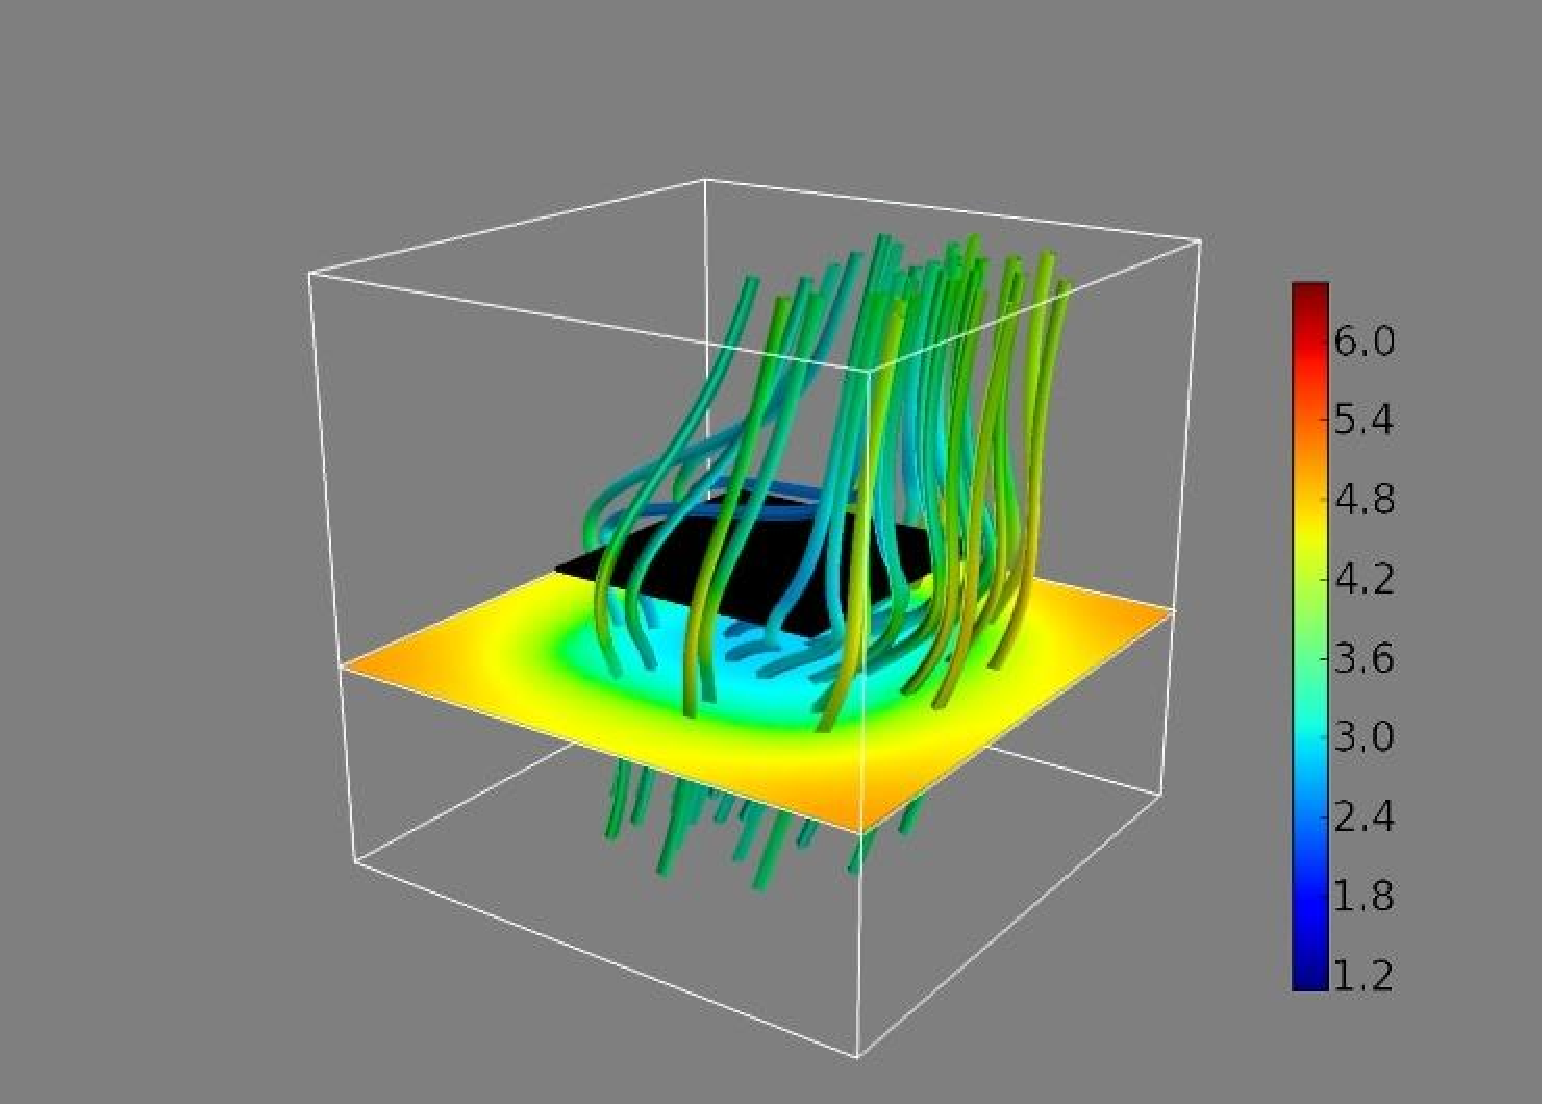
\includegraphics[bb=.0in .4in 11.5in 6.1in,width=4.355in,clip]{Images_Methodology/3dplot_50c.pdf}
		\hfill
		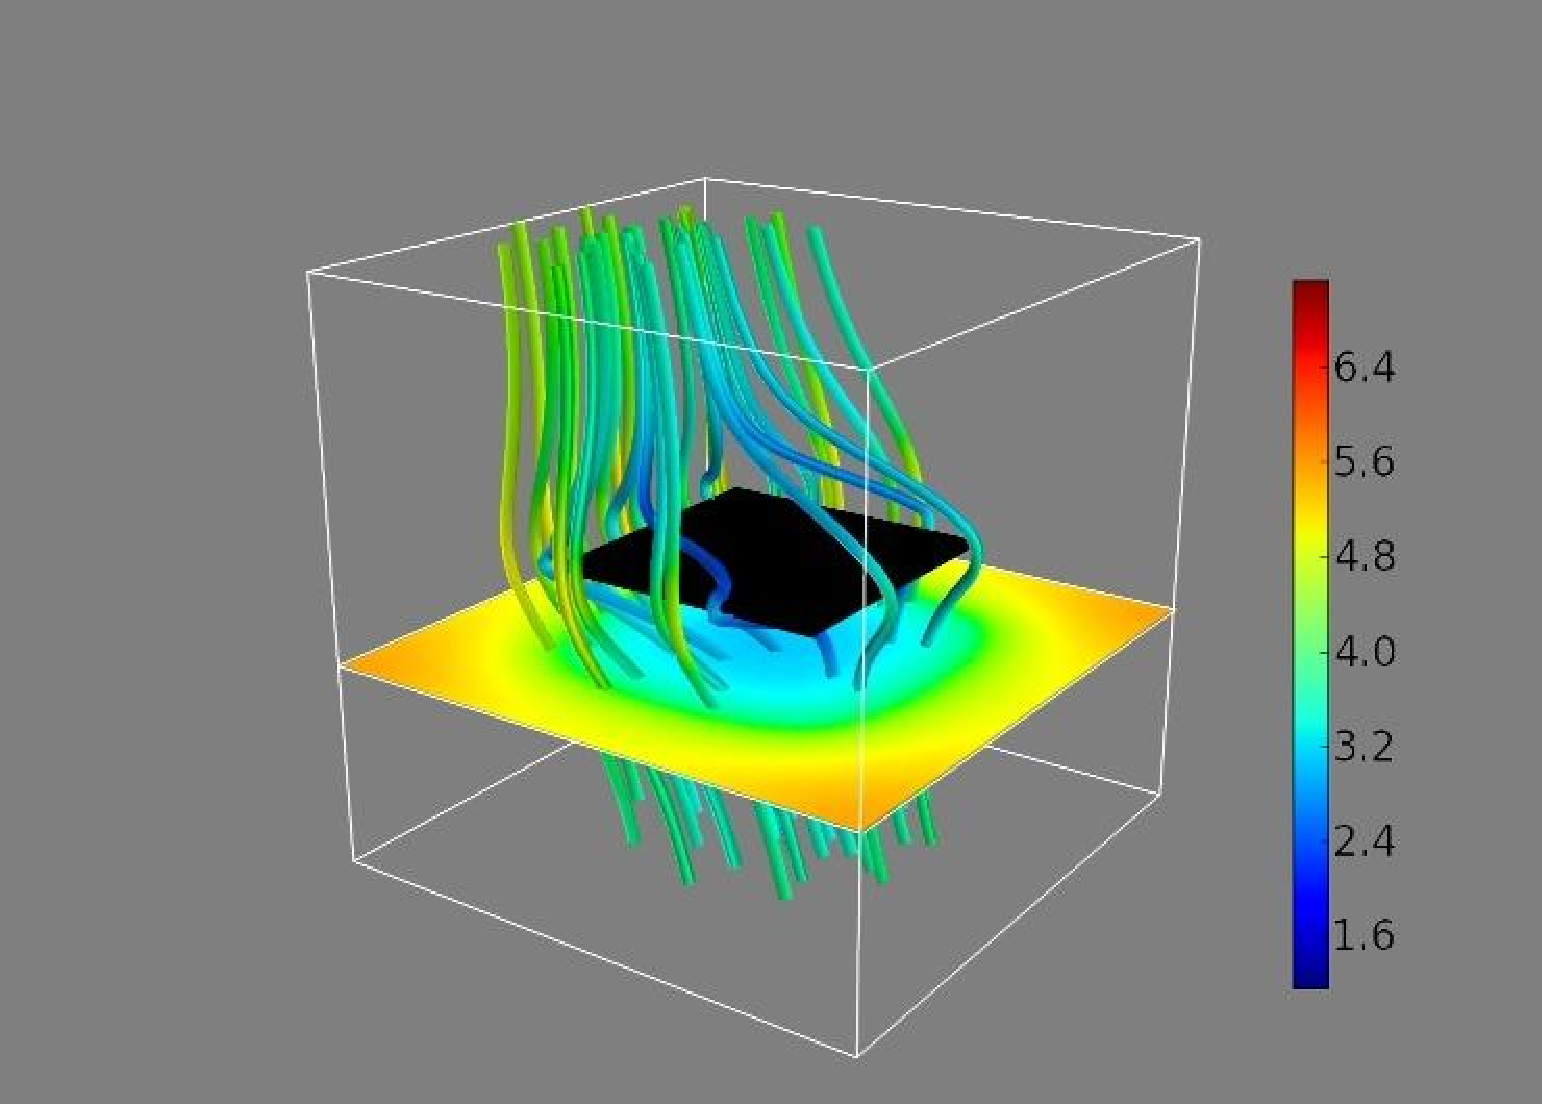
\includegraphics[bb=.0in .4in 11.5in 6.1in,width=4.35in,clip]{Images_Methodology/3dplot_72c.pdf}
		\hfill
		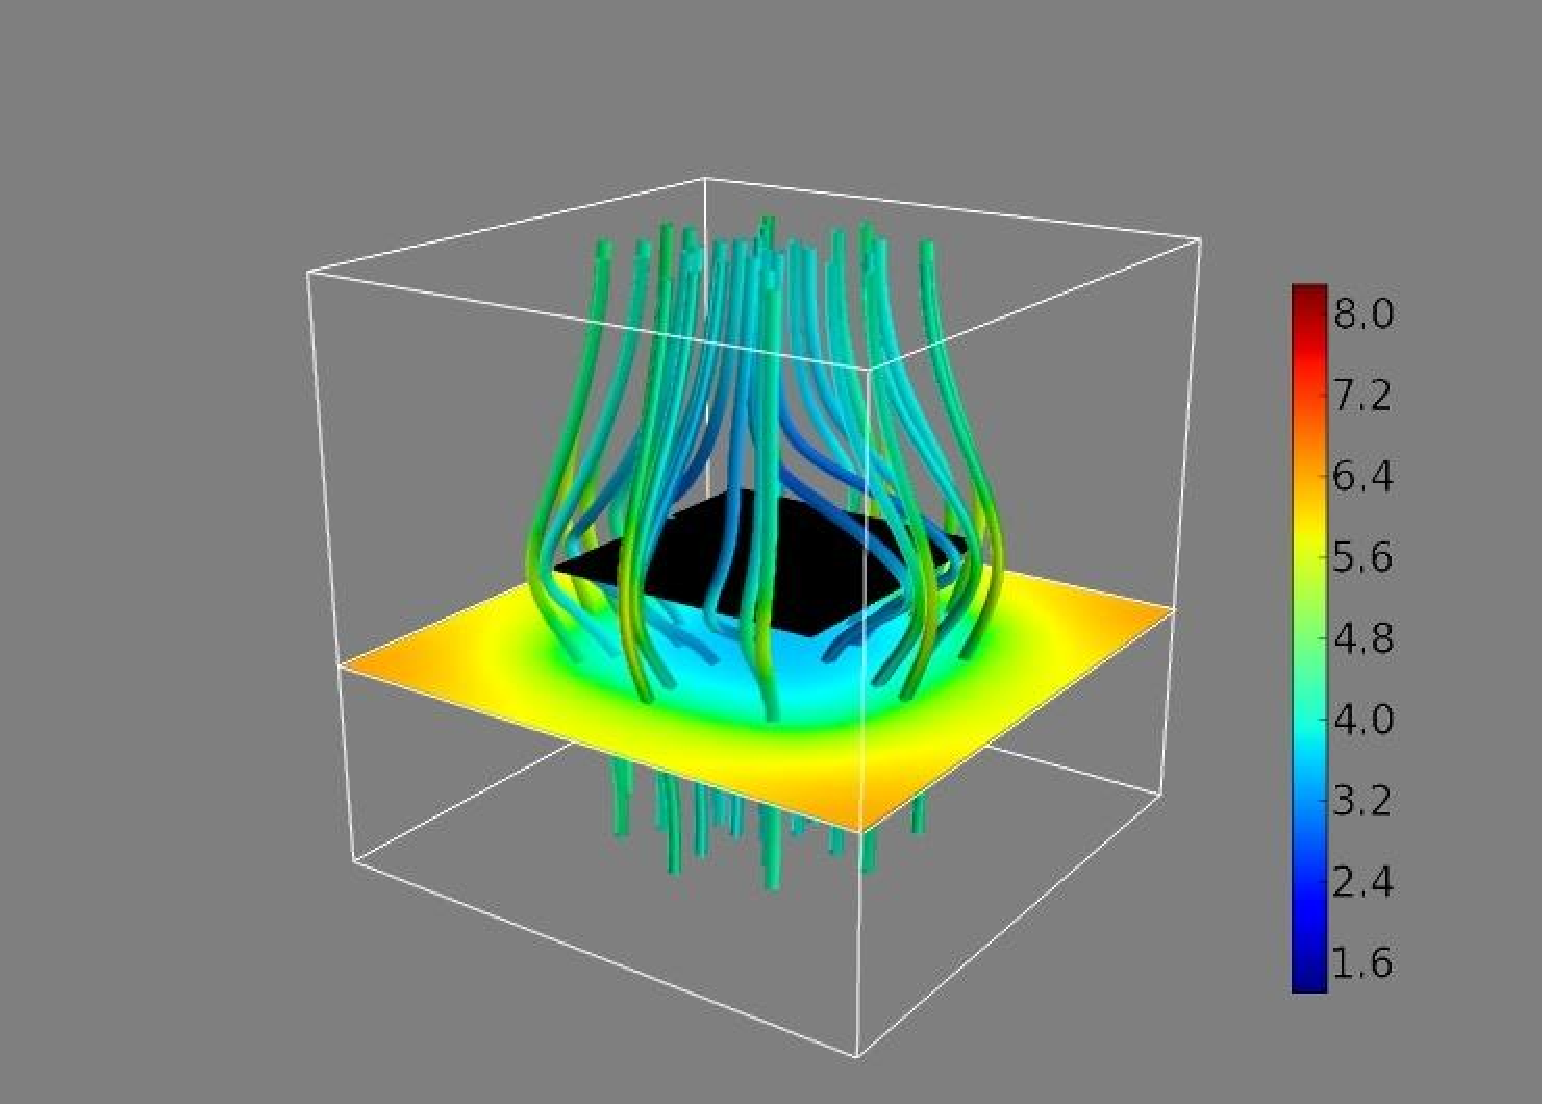
\includegraphics[bb=.0in .4in 11.5in 6.1in,width=4.355in,clip]{Images_Methodology/3dplot_104c.pdf}
	\end{center}
	\caption{\small Plot of the immersed plate with flow lines. The plate is drawn in black. Below the plate is a cross-section of the $z$-component of the velocity field with an associated color bar. $N=128$, and $N_B=8192$. Frames shown at total simulation time $T=0.020$, 0.142, and 0.208, from top to bottom.}
\label{fig:TimeProgression_Plate}
\end{figure}



\subsection{Case IV: An oscillating spheroid}

In the immersed plate test described above, the geometry of the structure is trivial and the deformations are negligible. 
Of course, the true power of the IB methodology lies in its seamless handling of both rigid {\em and} dynamic, flexible interfaces and in its structure-building capability. As an example of a simulation with a dynamic, flexible  interface we consider now an immersed, oscillating spheroid
given by
\begin{equation}
\frac{(x-0.5)^2}{(0.2+0.05\sin\theta(t))^2} +
\frac{(y-0.5)^2}{(0.2+0.05\sin\theta(t))^2} +
\frac{(z-0.5-0.05\cos\theta(t))^2}{(0.2-0.1\sin\theta(t))^2} = 1,
\label{meq:SphereEqn}
\end{equation}
where $\theta(t) = 2\pi t/T$, $t$ is the current simulation time and $T=0.25$ is the total simulation time. Equation (\ref{meq:SphereEqn}) yields a spheroid centered at $(0.5,0.5,0.5+0.05\cos\theta)$ with an equatorial radius of $0.2+0.05\sin\theta$ and a polar radius of $0.2-0.1\sin\theta$.
The prescribed motion induces a flow with a Reynolds number of about 10.

The shape of the spheroid is maintained by tethers. At time $t^n$ each fiber point $\B{X}^n_j$ is tethered to its respective location on the spheroid $\B{T}^n_j$. The sphere itself is discretized by triangulating a regular octahedron, yielding $N_B=578$, 2502, and 10406 fiber points when $N=32$, 64, and 128,  respectively. When solving for $\B{X}^{n+1}$ in the semi-implicit, lagged operators discretization, we take our initial guess to be $\B{X}^{n+1,0}=\B{T}^{n+1}$.
We use the same $0.0001$ convergence tolerance for CG as we do in the immersed plate simulation.

As in the previous example, we compare (explicit) FE/BE simulations with the proposed, fast, semi-implicit approach. For the FE/BE method the
stable timestep is determined by the empirical formula  $\Delta t = 0.5\cdot 10^{-1}h\sigma^{-1/2}$. Table~\ref{table:ExplicitTimestep_Sphere} provides a list of stable, explicit timesteps for this problem. 
\begin{table}
\caption{$\Delta t$ in the FE/BE explicit simulations of the immersed spheroid for various values of $N$ and $\sigma$. $\Delta t$ is approximately the largest stable timestep, given by the formula $\Delta t = 0.5\cdot 10^{-1}h\sigma^{-1/2}$.}
\label{table:ExplicitTimestep_Sphere}
\begin{center}

\begin{tabular}{c c c c c c}
  &  $\sigma=10^5$ & $\sigma=10^6$ & $\sigma=10^7$ & $\sigma=10^{8}$ & $\sigma=10^{9}$ \\
\cline{2-6}
\multicolumn{1}{c|}{$N=32$} & \TableTopSpace
4.941\e{-6} & 1.563\e{-6} & 4.941\e{-7} & 1.563\e{-7} & 4.941\e{-8} \\
\multicolumn{1}{c|}{$N=64$}  & \TableTopSpace
2.471\e{-6} & 7.813\e{-7} & 2.471\e{-7} & 7.813\e{-8} & 2.471\e{-8} \\
\multicolumn{1}{c|}{$N=128$} & \TableTopSpace
1.235\e{-6} & 3.906\e{-7} & 1.235\e{-7} & 3.906\e{-8} & 1.235\e{-8} \\
%\cline{2-6}
\end{tabular}

\end{center}
\end{table}
The required $\Delta t$  for a stable FE/BE simulation is even smaller than that in the plate example. Again, such direct, FE/BE simulations are impractical and would require a massive computational effort even for modest resolutions. 
For the implicit, lagged operators  discretization it is again sufficient to fix $\Delta t = 0.002$ to maintain both accuracy and stability for all resolutions,  $N=32$, 64, and 128. A comparison of the total CPU time for all simulations is presented in  
Table~\ref{table:SimulationTime_Sphere}. As in the plate example, the CPU time for the fast, semi-implicit simulations is almost invariant as 
 $\sigma$ increases.   The numbers are even more striking than in the preceding example; for $N=128$ and $\sigma=10^9$, the proposed approach is six orders of magnitude faster than the commonly used FE/BE approach.
\begin{table}
\caption{Total CPU time in hours for the explicit and semi-implicit simulations of the immersed spheroid, with varying values of $\sigma$. $^*$ denotes an extrapolated value.}
\label{table:SimulationTime_Sphere}
\begin{center}

\begin{tabular}{c c c c c c c}
  &  & $\sigma=10^5$ & $\sigma=10^6$ & $\sigma=10^7$ & $\sigma=10^{8}$ & $\sigma=10^{9}$ \\
\cline{3-7}
\multirow{2}{*}{$N=\hspace{1ex} 32$}
& \multicolumn{1}{c|}{Implicit} & \TableTopSpace
	0.013 & 0.015 & 0.015 & 0.016 & 0.016 \\
& \multicolumn{1}{c|}{Explicit} & \TableTopSpace
	4.405 & 13.675 & 43.467 & 135.742$^*$ & 429.701$^*$ \\
\vspace{.15 cm}
\\
  &  & $\sigma=10^5$ & $\sigma=10^6$ & $\sigma=10^7$ & $\sigma=10^{8}$ & $\sigma=10^{9}$ \\
\cline{3-7}
\multirow{2}{*}{$N=\hspace{1ex} 64$}
& \multicolumn{1}{c|}{Implicit} & \TableTopSpace
	0.127 & 0.134 & 0.140 & 0.138 & 0.137 \\
& \multicolumn{1}{c|}{Explicit} & \TableTopSpace
	83.155$^*$ & 253.626$^*$ & 822.769$^*$ & 2595.119$^*$ & 8213.271$^*$ \\
\vspace{.15 cm}
\\
  &  & $\sigma=10^5$ & $\sigma=10^6$ & $\sigma=10^7$ & $\sigma=10^{8}$ & $\sigma=10^{9}$ \\
\cline{3-7}
\multirow{2}{*}{$N=\hspace{1ex} 128$}
& \multicolumn{1}{c|}{Implicit} & \TableTopSpace
	1.057 & 1.125 & 1.141 & 1.151 & 1.167 \\
& \multicolumn{1}{c|}{Explicit} & \TableTopSpace
	1326.0$^*$ & 4170.7$^*$ & 13904.8$^*$ & 43827.9$^*$ & 134516.2$^*$ \\
\end{tabular}
   
\end{center}
\end{table}
A depiction of the flow obtained using the new fast, semi-implicit approach  is presented in Figure~\ref{fig:TimeProgression_Sphere}. 
 \begin{figure}[htb]
	\begin{center}
		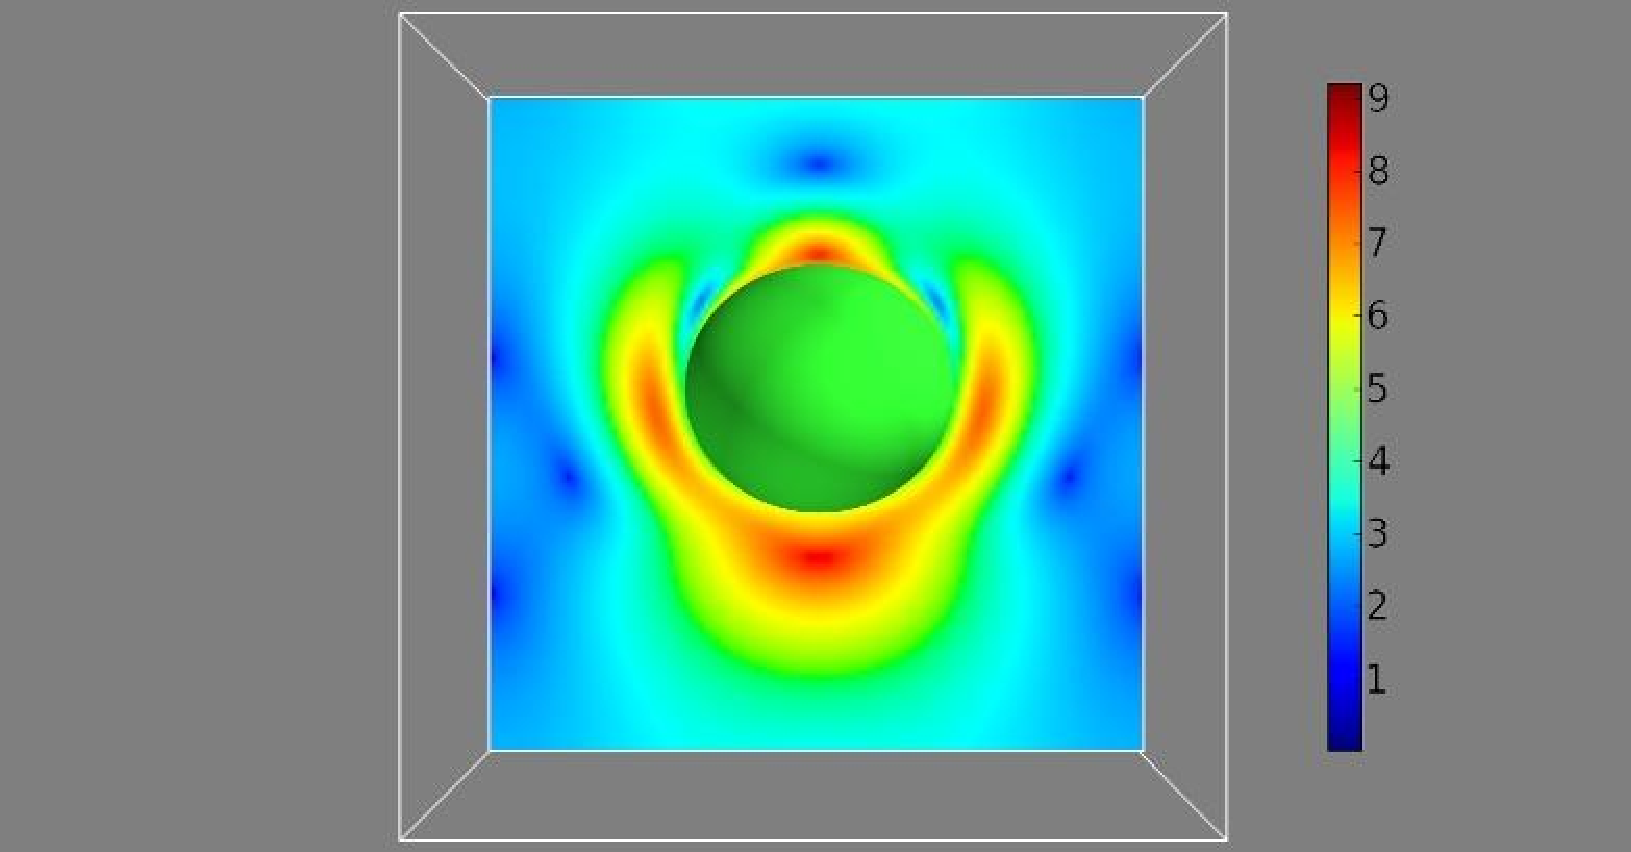
\includegraphics[bb=.0in .4in 11.5in 6.1in,width=4.4in,clip]{Images_Methodology/SpherePlot_3c.pdf}
		\hfill
		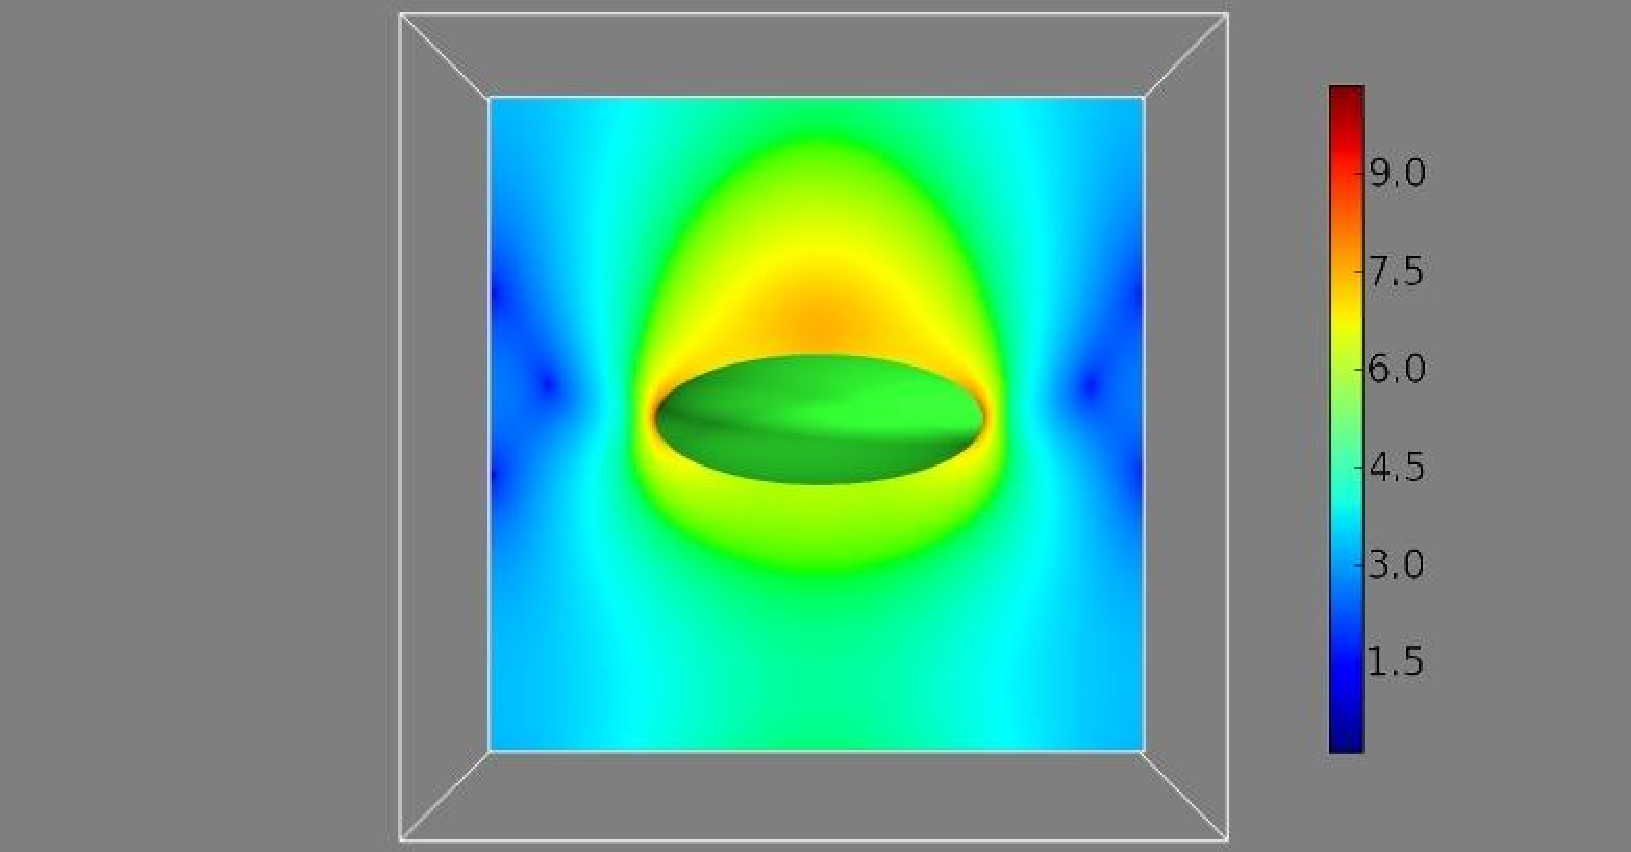
\includegraphics[bb=.0in .4in 11.5in 6.1in,width=4.4in,clip]{Images_Methodology/SpherePlot_31c.pdf}
		\hfill
		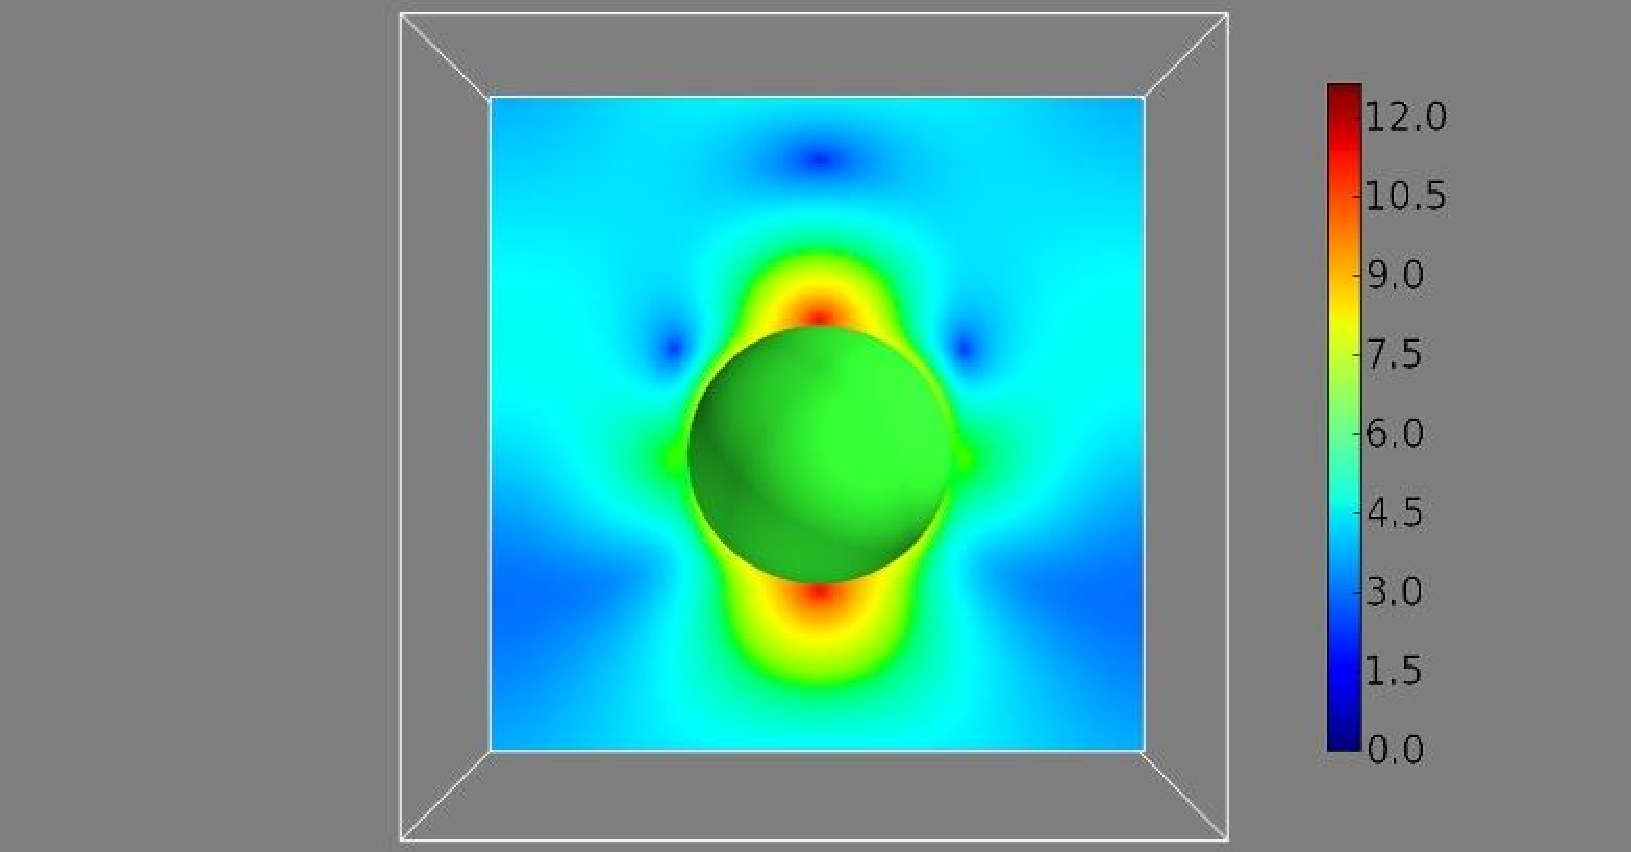
\includegraphics[bb=.0in .4in 11.5in 6.1in,width=4.4in,clip]{Images_Methodology/SpherePlot_63c.pdf}
	\end{center}
	\caption{\small Plot of the immersed spheroid, drawn in green. Cutting the spheroid is a cross-section of the velocity magnitude scalar field with an associated color bar. $N=128$, and $N_B=10406$. Frames shown at total simulation time $T=0.006$, 0.062, and 0.126, from top to bottom.}
\label{fig:TimeProgression_Sphere}
\end{figure}



\subsection{Accuracy}
There are a number of differences between our implicit methodology and the standard FE/BE explicit methodology. Each difference is a potential source of additional numerical error: the larger timestep taken, the implicit discretization itself, the assumption of translation invariance of $G_h$, the trilinear interpolation used to calculate values of the form $G_h(\B{z})$, the far field expansion of $G_h$, and approximate nature of  the Krylov subspace solvers. We have been extra careful to ensure that each of these errors is 
 no more than $O(h)$, the underlying order of the IB Method, and to verify numerically that these errors do not accumulate. 
 
To analyze error accumulation we again turn to our simulations of a plate and a sphere. For the following simulations we fix the immersed structure via tether points with spring constant $\sigma=10^6$ and induce a simple flow by adding a constant force $\B{f} = (0,0,1)$ to every point of the fluid domain. We perform the simulation first for $N=128$ using the explicit method and store the resulting fluid velocity at time $T=0.1$ as $u_{128}$. This velocity field will serve as a our standard by which we gauge the accuracy of other simulations.

We now perform the same simulation twice for $N=32$, $64$, and $96$, once using the explicit method and once using our implicit methodology. We calculate the relative error between a velocity field $\tilde{u}$ and our standard $u_{128}$ by taking the $l^2$-norm, $\norm{u_{128} - \tilde{u}}_{l^2} / \norm{u_{128}}_{l^2}$. For simplicity we downsample all velocity fields to a $32\times 32\times 32$ grid. The resulting errors can be seen in Table~\ref{table:TotalError}.

The relative errors from our implicit simulations are roughly the same as those from the explicit simulations, confirming that our fast implicit methodology is not generating any unacceptable inaccuracies.


Finally, we perform one more test to verify that approximating $G_h$ as translation invariant does not lead to a degradation of the overall accuracy. We do a simulation using an identical setup as that used for the calculation of $u_{128}$, except we shift the immersed boundary upward by a distance of $h/2$. We store the resulting fluid velocity at time $T=0.1$ as $\tilde{u}_{128}$.

If $G_h$ were exactly translation invariant then the resulting simulation would be identical to the original simulation up to a shift of the velocity field. That is, we would have $u_{128}(\B{z}) = \tilde{u}_{128}(\B{z} + (0,0,h/2))$, for any $\B{z}\in\Omega_h$. This is the case with the continuous equations.

For our discrete simulations $G_h$ is not exactly translation invariant and there is a difference between $u_{128}(\B{z})$ and $\tilde{u}_{128}(\B{z} + (0,0,h/2))$. Note that we use simple linear interpolation to calculate values of $\tilde{u}_{128}$ between grid points. 
Calculating the relative difference between $u_{128}$ and a shifted $\tilde{u}_{128}$  using the $l^2$-norm as before, we see that this difference is less than 1\%, or smaller than the error of the method. Shifts other than $(0,0,h/2)$ yield similar results.


\begin{table}
\caption{The relative error between various low resolution simulations and a high resolution explicit simulation.}
\label{table:TotalError}
\begin{center}

\begin{tabular}{c c c c c}
  &  & $N=32$ & $N=64$ & $N=96$ \\
\cline{3-5}
\multirow{2}{*}{Plate}
& \multicolumn{1}{c|}{Implicit} & \TableTopSpace
   0.160 & 0.0327 & 0.015 \\
& \multicolumn{1}{c|}{Explicit} & \TableTopSpace
   0.222 & 0.073 & 0.024 \\
\vspace{.15 cm}
\\
  &  & $N=32$ & $N=64$ & $N=96$ \\
\cline{3-5}
\multirow{2}{*}{Sphere}
& \multicolumn{1}{c|}{Implicit} & \TableTopSpace
	0.058 & 0.015 & 0.005 \\
& \multicolumn{1}{c|}{Explicit} & \TableTopSpace
  0.089 & 0.029 & 0.009 \\
\vspace{.15 cm}
\end{tabular}
   
\end{center}
\end{table}

\section{Conclusion}
In Chapter~\ref{part:Matrix}, novel expedited methods for  the semi-implicit system (\ref{meq:dmoment})-(\ref{meq:Xt}) were proposed. We showed that these methods were highly efficient for many 2D applications.
The cost of the implicit solvers presented were on the order of the cost of a fluid solve, allowing for efficient implicit timestepping with computational cost on the same order as that of an explicit timestep. The direct extension of that methodology to 3D was unfeasible due to the large number of fiber points common to 3D IB applications.

In this chapter we presented an entirely new, alternative methodology suitable for the 3D case and for when there is a large number of immersed boundary points. We showed that the efficiency of the proposed  fast  semi-implicit solver,  relative to the cost of a fluid solve,  is asymptotically superior to the solvers in the 2D case. Indeed, in our test problems, we demonstrated that solving the implicit system was not the predominant cost for the semi-implicit timestep, but was rather overshadowed by the cost of the necessary fluid solves. Thus, we have  shown that the stiffness inherent in many IB applications can be eliminated via a  robust, semi-implicit discretization  for a minimal cost. More importantly, the proposed approach scales very well as $N_B$ increases, allowing the new methodology to be applied to a wide range of complex structures.
The computational savings obtained with the new methodology are enormous. IB Method computations that would typically require weeks or months using the  standard, FE/BE approach can now be performed in just minutes.






\chapter{The Splitting Method}
\label{part:Splitting}
\noindent
In Chapter~\ref{part:Matrix} and~\ref{part:Treecode} we focused on methods to accelerate computations of the form $\C{M}_n\B{F}$, as well as iterative methods to solve the linear system (\ref{meq:Xnl}) in the case that $\C{A}_{h_B}$ or its Jacobian, $J$, is negative-semidefinite. In the more difficult case that $J$ is nondefinite we must find alternative iterative methods to solve (\ref{meq:Xnl}).

In this chapter we explore a special case where $J$ is nondefinite but has eigenvalues that are all large in magnitude. This case includes applications modeling rigid bodies. We will develop the methodology, known as the Splitting Method, in conjunction with a specific application, namely flow past a rigid valve.

\section{Case V: A model of a heart valve}
\label{Sec:valve}
\subsection{The model}
We turn now to a more challenging application of the IB Method in which there are rigid immersed
structures, tethered points, and crossed links. 
We consider a 2D model of a rigid valve immersed in blood flowing through an artery. The valve is indirectly restricted in motion by two hinges but is allowed to rotate. The valve, artery walls, and hinges will all be modeled as immersed springs. The flow-structure interaction will be captured 
via the IB Method.


We select the computational domain to be $\Omega=[0,2]\times[0,1]$  with periodic boundary conditions and  discretize it with a $2N\times N$ uniform grid. The geometry of the problem is
represented in Fig.~\ref{fig:ValveGeometry} and a detailed depiction of the valve's linked structure is shown in Fig.~\ref{fig:Valve1}. The top and bottom of the artery walls include cushions in the shape of two hills. We simulate a horizontal flow through the artery by adding a forcing vector $\B{f}_{j,k}=(v_{flow},0)$ to the right hand side of (\ref{meq:dmoment}), where in general $v_{flow}$ may be time dependent. This changes the explicit term $\B{b}^n$ in our implicit system to
\begin{equation}
\B{b}^n=\B{X}^n + \Delta t\C{S}^*_n\C{L}_h
\left[ \B{u}^n - \Delta t\B{u}^n \cdot \nabla_h \B{u}^n + \frac{\Delta t}{\rho} \B{f} \right].
\end{equation}
\begin{figure}[!b]
  \begin{center}
   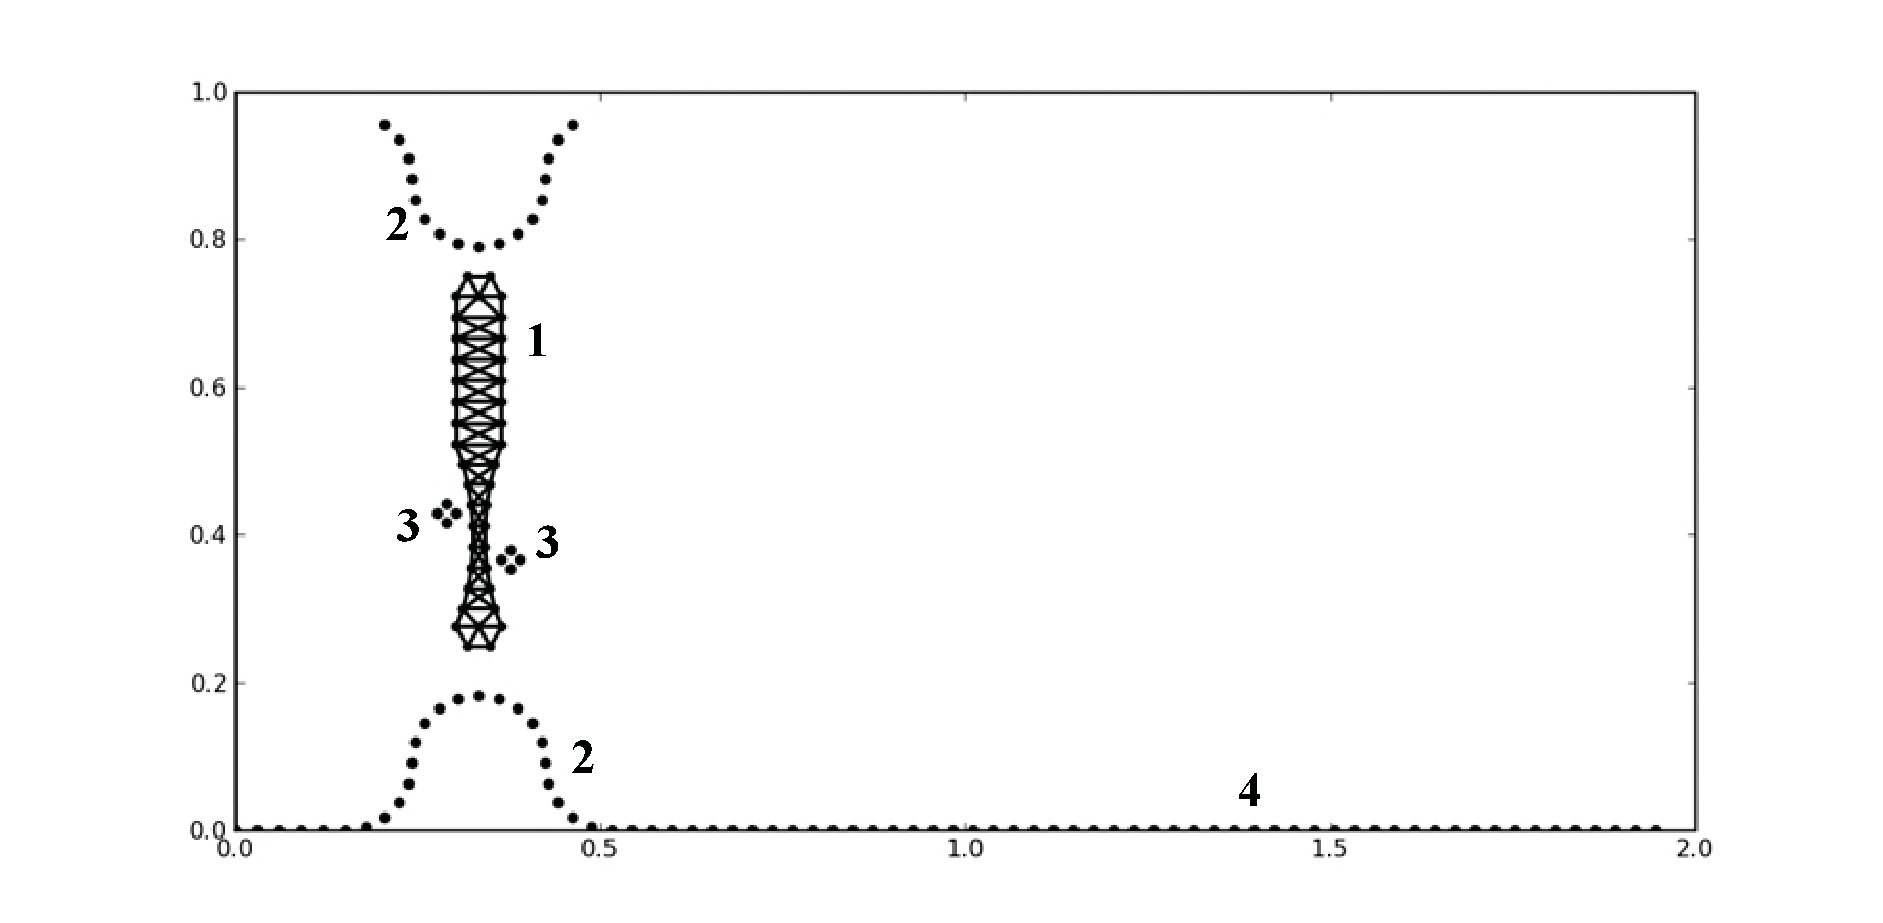
\includegraphics[bb=1in .3in 11.5in 5.85in,width=5.25in,clip]{Images_Methodology/ValveGeometry.pdf}
  \end{center}
  \caption{\small Configuration of heart valve model. Larger nodes represent tether points. 1: Valve; 2: Cushions; 3: Hinges; 4: Artery wall.}
  \label{fig:ValveGeometry}
\end{figure}
\begin{figure}[!b]
  \begin{center}
    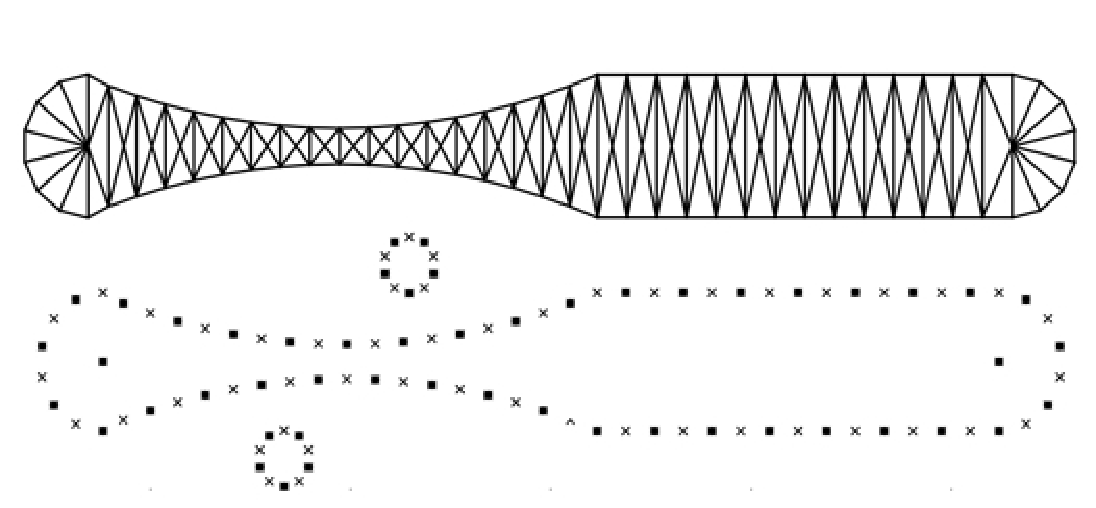
\includegraphics[bb=0in 0in 7.25in 3.3in,width=5.25in,clip]{Images_Methodology/Valve1.pdf}
  \end{center}
  \caption{\small Top: A fine grid approximation to the valve, showing only linkage. Bottom: 'x's mark the prolongation of a coarse valve marked in 'o'.}
  \label{fig:Valve1}
\end{figure}

All nodes in the wall and the two hinges are modeled as tethers, with one end of the tether fixed for all time. If $\B{X}_i$ is a tethered point with base given by $\bar{\B{X}}_i$ then the force generated by the tether is given by 
\begin{equation}
\B{f}_i = -k_i (\B{X}_i-\bar{\B{X}}_i)
\label{eqn:TetherForce}
\end{equation}
where $k_i$ is the spring constant. For the body of the heart valve we will use springs between nodes. Suppose $\B{X}_i$ is connected to multiple other nodes. If $\B{X}_i$ is connected to $\B{X}_j$ then let $k_{i,j}$ and $L_{i,j}$ be respectively the spring constant and resting length of the spring connecting them. If no connection exists between $\B{X}_i$ and $\B{X}_j$ then take $k_{i,j}$ to be zero. The force at $\B{X}_i$ then is given by
\begin{equation}
\B{f}_i = \sum_{j=1}^{N_B} -k_{i,j} \frac{\B{X}_i-\B{X}_j}{|\B{X}_i-\B{X}_j|}
(|\B{X}_i-\B{X}_j| - L_{i,j}).
\label{eqn:LinkForce}
\end{equation}
Note that the force operator (\ref{eqn:LinearForce}) employed for the elliptical membrane problem 
is exactly the force given by (\ref{eqn:LinkForce}) for a loop of fiber points connected sequentially by springs with suitable spring constants and zero resting length. 
However, for our valve model we require non-zero resting lengths to preserve the structure and as a consequence we end up with a nonlinear force density.
Additionally, the problem is severely stiff. To maintain the rigidity of a solid body,  we find that the
 spring constants must be $O(10^9h^{-2})$. Similarly, for the tether points representing the artery walls, the spring constants must also be very large to portray the tautness of the biological fibers. Furthermore, because the forcing flow acts to bend the valve as it is penned between its hinges,  larger values of $v_{flow}$ require larger spring constants to preserve the structure. 
To illustrate the stiffness, a time integration of the equations of motion with an explicit treatment 
of the interfacial force and with a modest spatial resolution ($N=256$) requires the time-step to be 
$O(10^{-7})$.  

 Removing this stiffness for this more prototypical IB Method problem is considerably  more challenging than in the case of the simple elliptical fiber. The implicit system we would like to solve is still given 
 by~(\ref{meq:Xnl}):
$$
\B{X}^{n+1} = \C{M}_n\C{A}_{h_B} (\B{X}^{n+1}) + \B{b}^n.
$$
As noted above, due to the nonzero resting lengths of the springs comprising the valve, 
$\C{A}_{h_B}$ is nonlinear. Moreover, unlike the case of the elliptical interface with
nonlinear force density,  the Jacobian $J$ of $\C{A}_{h_B}$ is not semidefinite and the resulting matrix $I - M_nJ$ can be shown to lack definiteness as well.

The breakdown of the definiteness of $J$ can be seen in a very simple case. Consider four immersed boundary points at $(1,0),(0,1),(-1,0),(0,-1)$, forming a square with side lengths $\sqrt{2}$ and with links connecting the perimeter of the square. We vary the resting length $l$ of the connecting springs and compute the eight eigenvalues of the resulting force density's Jacobian. The results are plotted in
Fig.~\ref{fig:BoxEigenvalues}. We see that as the resting length approaches and surpasses the side length of the square the Jacobian loses its negative semi-definiteness. This seems to be generic
for most immersed structures. For our 2D valve model, we take the resting length to be the starting length of the links comprising the valve. Thus,  we  lose immediately negative semi-definiteness once we perturb the valve structure.

Due to the lack of positive definiteness of $I-M_nJ$  the Conjugate Gradient Method does not converge. The Biconjugate Gradient Method converges but may take in excess of $100$ iterations to attain a satisfactory residual. A major obstacle in accelerating convergence is that the natural preconditioner $I-M_n'J$ (where $M_n'$ is the diagonal part of $M_n$) does not capture well the dynamics of this system. Indeed, Jacobi iterations have very poor convergence, requiring strong underrelaxation and thousands of iterations. Without adequate smoothers, an efficient  multigrid for the linear system in Newton's iteration is not a viable option. Smoothers for the nonlinear system (\ref{meq:Xnl}) were likewise difficult to uncover, seemingly ruling out a nonlinear multigrid. We propose next a very different approach,  which consists of splitting the 
problem to take simultaneous advantage of the fast convergence of Newton's method and the efficiency of multigrid. 
\begin{figure}[!b]
  \begin{center}
    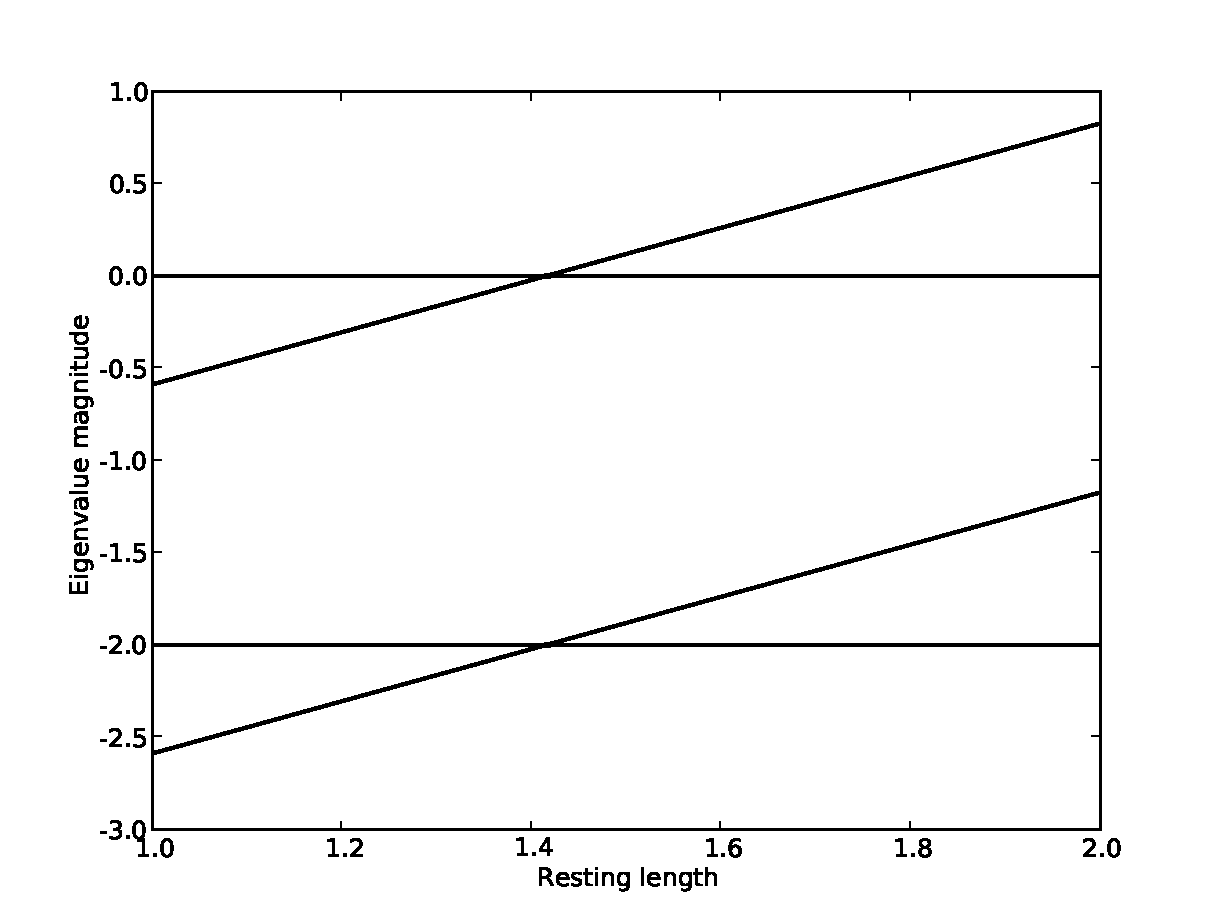
\includegraphics[bb=.15in .15in 8in 6in,width=5.25in,clip]{Images_Methodology/BoxEigenvalues.pdf}
  \end{center}
  \caption{\small Eigenvalues for the Jacobian of a fiber forcing function for four points linked as a square with varying resting length.}
  \label{fig:BoxEigenvalues}
\end{figure}

\subsection{Solving the implicit system via fixed point iterations}
Perhaps the simplest iterator for (\ref{meq:Xnl}) is the fixed point iteration given by
\begin{equation}
\B{X}^{n+1,k+1} = \mathit{M}_n\C{A}_{h_B} (\B{X}^{n+1,k}) + \B{b}^n.
\label{eqn:fixedpoint}
\end{equation}
However, this method fails spectacularly. This is not entirely surprising.
 If our initial guess is $\B{X}^{n+1,0}=\B{X}^n$ then $\B{X}^{n+1,1}$ is the explicit update provided by the FE/BE scheme which is unstable for practical $\Delta t$. Additional iterations of (\ref{eqn:fixedpoint}) exacerbate the instability: small errors in $\B{X}^{n+1,k}$ are amplified enormously by $\C{A}_{h_B}$ resulting in large errors in $\B{X}^{n+1,k+1}$.

The eigenvalues of $J$ are at least on the order of the spring constants comprising our valve. It should seem natural to take advantage of this by reversing the fixed point iteration (\ref{eqn:fixedpoint}). Consider the alternative fixed point iteration
\begin{equation}
\left\{
\begin{gathered}
\mathit{M}_n\B{F}^{k+1} = \B{X}^{n+1,k} - \B{b}^n,\\
\C{A}_{h_B}(\B{X}^{n+1,k+1}) = \B{F}^{k+1}.
\end{gathered}
\right.
\label{eqn:fixedpoint2}
\end{equation}
First, we solve for $\B{F}^{k+1}$, the force distribution that would move the fiber from $\B{X}^n$ to $\B{X}^{n+1,k}$ after a single timestep. The linear system we must solve only involves the linear positive definite operator $\C{M}_n$, thus we can efficiently solve it using (linear)multigrid. Second, we determine what configuration $\B{X}^{n+1,k+1}$ gives rise to this force through $\C{A}_{h_B}$.
In many applications there is a unique $\B{X}^{n+1,k+1}$ such that
$\C{A}_{h_B}(\B{X}^{n+1,k+1}) = \B{F}^{k+1}$. For the current problem this is not the case.

To see this note that valve is modeled as a neutrally buoyant object, detached from any fixed points, and the internal forces generated by perturbations in the valve's structure are unaffected by translation. More precisely let $\C{G}_V$ be all indices $l$ such that $\B{X}_l$ is a fiber point belonging to the valve. We consider then two translation vectors $\B{V}^1$ and $\B{V}^2$ given by
\begin{equation}
\B{V}^1_l =
\begin{cases}
(1,0)& \textrm{if } l\in \C{G}_V, \\
(0,0)& \textrm{otherwise},
\end{cases}
\end{equation}
\begin{equation}
\B{V}^2_l =
\begin{cases}
(0,1)& \textrm{if } l\in \C{G}_V, \\
(0,0)& \textrm{otherwise}.
\end{cases}
\end{equation}
$\B{V}^1$ and $\B{V}^2$ are horizontal and vertical translation vectors, $\B{X}+\B{V}^1$ representing the same configuration as $\B{X}$ with the valve shifted right by one unit. Shifting has no influence on the force density,
\begin{equation}
\C{A}_{h_B}(\B{X}+a_1 \B{V}^1) = \C{A}_{h_B}(\B{X}+a_2 \B{V}^2) = \C{A}_{h_B}\B{X},
\end{equation}
where $a_1$ and $a_2$ are arbitrary scalars.
Thus,  $\C{A}_{h_B}$ is not injective and we may not have a unique solution to (\ref{eqn:fixedpoint2}). In fact, $\C{A}_{h_B}$ is not surjective either so (\ref{eqn:fixedpoint2}) may have no solution at all. This follows physically from conservation of linear momentum and angular momentum: $\C{A}_{h_B}$ cannot directly generate forces that move or rotate the valve. Translation and rotation can only be introduced via the fluid interaction. 

To analyze rotation we introduce the operator $R_{\theta}$ which takes in a configuration $\B{X}$ and returns the configuration obtained by rotating the valve by $\theta$ about some fixed point. This point of rotation is arbitrary and we take it to be the center of the valve at the previous time-step:
\begin{equation}
\B{x}_c = 
\left(\frac{( \B{X}^n, \B{V}^1)_B}{( \B{V}^1, \B{V}^1)_B}, 
\frac{( \B{X}^n, \B{V}^2)_B}{( \B{V}^2, \B{V}^2)_B}\right).
\label{eqn:Center}
\end{equation}
We define also
\begin{equation}
\B{V}^3(\B{X}) = \frac{\partial}{\partial \theta}R_\theta(\B{X}). 
\label{eqn:e3}
\end{equation}
We may equivalently define $\B{V}^3$ via
\begin{equation}
\B{V}^3_l =
\begin{cases}
(-Y_l+y_c,X_l-x_c)& \textrm{if } l\in \C{G}_V, \\
(0,0)& \textrm{otherwise},
\end{cases}
\end{equation}
where $\B{X}_k=(X_k,Y_k)$ and $\B{x}_c = (x_c,y_c)$. $\B{V}^3$ is the Jacobian of $R_\theta$. Note that $\B{V}^3$ depends on a configuration $\B{X}$. We use the
notation $\B{V}^3(\B{X})$ to emphasize this dependence.

The vectors $\B{V}^1,\B{V}^2,\B{V}^3$ represent points outside the image of $\C{A}_{h_B}$ associated with translation and rotation. Then, 
we have that there exist solutions to (\ref{eqn:fixedpoint2}) only when $\B{F}^{k+1}$ does not act to translate or rotate the valve. That is, a vector $\B{F}$ lies in the image of $\C{A}_{h_B}$ only when 
\begin{equation}
( \B{F}, \B{V}^j )_B = 0 \quad
\textrm{ for } j=1,2,3.
\label{eqn:FCondition}
\end{equation}
Indeed, consider first the simplest case of only two immersed fiber points
\begin{equation}
\B{X}=
\left( \begin{array}{c}
(x_1,y_1)\\
(x_2,y_2)
\end{array} \right)
\end{equation}
connected with a single link. Then,  the force they generate is
\begin{equation}
\B{F}=T
\left[ \begin{array}{c}
(x_2-x_1,y_2-y_1)\\
(x_1-x_2,y_1-y_2)
\end{array} \right]
\end{equation}
for some tension scalar $T$.
The rotation vector about the origin is simply 
\begin{equation}
\B{V}^3=
\left[ \begin{array}{c}
(-y_1,x_1)\\
(-y_2,x_2)
\end{array} \right].
\end{equation}
We have then that
\begin{equation}
( \B{F},\B{V}^3 )_B =
-y_1(x_2-x_1) + x_1(y_2-y_1) - y_2(x_2-x_1) + x_2(y_1-y_2) = 0.
\end{equation}
A similar calculation shows that $( \B{V}^1,\B{F} )_B = ( \B{V}^2,\B{F} )_B = 0$.
For our more complicated valve structure  we simply have a summation of such forces, thus the
corresponding  force density must satisfy (\ref{eqn:FCondition}) where 
$\B{F}=\C{A}_{h_B}(\B{X})$ for any configuration $\B{X}$. In general, an arbitrary vector $\B{F}$ may not satisfy (\ref{eqn:FCondition}) and we would be unable to find a solution to (\ref{eqn:fixedpoint2}). To remedy this we must factor out those components  outside the image of $\C{A}_{h_B}$. This is easier to do with the linearized $\C{A}_{h_B}$, its Jacobian, where we may simply project onto the vector space free of the problematic vectors $\B{V}^1,\B{V}^2,\B{V}^3$. These 
observations suggest the modified Newton iteration to approximately solve for $\B{X}^{n+1,k+1}$ in (\ref{eqn:fixedpoint2}):
\begin{equation}
\left\{
\begin{gathered}
\B{X}^{n+1,k+1,0} = \B{X}^{n+1,k} , \\
\begin{aligned}
J(\B{X}^{n+1,k+1,l})(\B{X}^{n+1,k+1,l+1}& - \B{X}^{n+1,k+1,l})   \\
& = P(\B{F}^{k+1} - \C{A}_{h_B}(\B{X}^{n+1,k+1,l})),
\end{aligned}
\end{gathered}
\right.
\label{eqn:AnewtonProj}
\end{equation}
where
\begin{equation}
P(\B{F}) = \B{F} - \sum_{j=1}^3 \B{V}^j(\B{X}^{n+1,k})(\B{F},\B{V}^j(\B{X}^{n+1,k}))_B 
\label{eqn:project}
\end{equation}
is the projection operator onto rotation and translation free force distributions. Note that because each node in the valve is linked to only a few other nodes, $J$ is $O(N_B)$ sparse. We can solve systems involving $J$ efficiently with various sparse solvers. Additionally, the structure of $J$ never changes throughout a simulation, though its values do, so we may make additional optimizations in the sparse solver if desired.

Linear systems of the form $J\B{X}=P\B{F}$ are, strictly speaking, over determined by three degrees of freedom. To rectify this we simply isolate three degrees of freedom in $\B{X}$ and fix them. These variables must be associated with the valve but are otherwise arbitrary. We could, for instance, fix the $x$ and $y$ component of a single node in the valve as well as the $x$ component of an additional node. Once fixed,  we may proceed to solve for $\B{X}$ such that $J\B{X}=P\B{F}$ is satisfied at all other free points. What is important, however, is that iterations of (\ref{eqn:AnewtonProj}) in such a manner will converge to an $\B{X}$ that satisfies $\C{A}_{h_B}\B{X}=P\B{F}$ at all points, even at those we fixed. In this sense we arrive at an updated configuration $\B{X}^{n+1,k+1}$ which satisfies (\ref{eqn:fixedpoint2}) up to components outside the image of $\C{A}_{h_B}$.

The sequence $\B{X}^{n+1,0}, \B{X}^{n+1,1}, \B{X}^{n+1,2}, \dots$ formed by iterations of (\ref{eqn:fixedpoint2}) typically converges quadratically in the $l^2$ norm.
As an aside, it is important to note that the iterative method (\ref{eqn:fixedpoint2}) converges precisely because the standard fixed point iteration (\ref{eqn:fixedpoint}) diverges. As we modify the parameters of our simulation, for instance,  if we were to drastically decrease the spring constants, then (\ref{eqn:fixedpoint}) may converge whereas (\ref{eqn:fixedpoint2}) would diverge. There are situations with mixed large and small spring constants where neither iteration converges. The crosslinks of our valve model is one such example. In the case of large spring constants everywhere (\ref{eqn:fixedpoint2}) converges rapidly and increasing the spring constants aids in the convergence.

The limit of our iterations is a stable update of the immersed boundary configuration but is not in general a solution to (\ref{meq:Xnl}). We need to reintroduce translation and rotation to correct for this 
discrepancy. We can achieve this in many different ways. Perhaps the simplest method is  to use the location and angle of the valve configuration obtained from an explicit update. To accomplish this we may simply take our initial guess $\B{X}^{n+1,0}$ for iterations of (\ref{eqn:AnewtonProj}) to be
\begin{equation}
\B{X}^{n+1,0} = R_{\theta}\B{X}^n + \B{V}^1(\tilde{\B{X}}-\B{X}^n,\B{V}^1)_B
+ \B{V}^2(\tilde{\B{X}}-\B{X}^n,\B{V}^2)_B
\label{eqn:InitialGuess}
\end{equation}
where
\begin{equation}
\theta = (\tilde{\B{X}}-\B{X}^n
-\B{V}^1(\tilde{\B{X}}-\B{X}^n,\B{V}^1)_B
-\B{V}^2(\tilde{\B{X}}-\B{X}^n,\B{V}^2)_B
,\B{V}^3(\B{X}^n))_B
\end{equation}
and
\begin{equation}
\tilde{\B{X}} = \B{X}^n + \C{M}_n\C{A}_{h_B}\B{X}^n
\end{equation}
Here, we are taking the FE/BE predictor $\tilde{\B{X}}$ and extracting its location and angle. We then take the current configuration $\B{X}^n$ and modify the location and angle of the valve to match that in $\tilde{\B{X}}$. After this, 
 we may proceed to apply iterations of (\ref{eqn:AnewtonProj}) which will preserve the location and angle we extracted from the FE/BE predictor.

Other predictors may be employed as well. 
For instance we may rediscretize our problem on a coarser grid, solve for the updated time-step, prolong the solution to the original fine grid and extract its gross properties. 
%In fact solving (\ref{eqn:fixedpoint2}) via iterations of (\ref{eqn:AnewtonProj}) is a good nonlinear smoother, opening the possibility for a nonlinear multigrid. 
Other predictors may involve higher order explicit updates $\tilde{\B{X}}$ or treating the valve as a true rigid body and predicting its motion through rigid body motion. 

\subsection{Reintroducing translation and rotation iteratively}
Many of the explicit predictors, such as those discussed above,  behave quite satisfactorily and in conjunction with  (\ref{eqn:fixedpoint2}) provide accurate and stable solutions to (\ref{meq:Xnl}). 
 In a number of applications this is sufficient. If we employ (\ref{eqn:AnewtonProj}) after using the initial guess (\ref{eqn:InitialGuess}) we can obtain efficiently an approximate  solution to (\ref{meq:Xnl}) within truncation error with just a few iterations.

In the current application, however, extra care must be taken. The close proximity of the valve to its hinges can quickly lead to unphysical collisions  if small errors in translation propagate throughout the simulation. 
This proximity can also seriously affect the behavior of an explicit predictor, leading to highly inaccurate translation and rotation.
Of course, even exact solutions to (\ref{meq:Xnl}) with $\Delta t$ large may still produce collisions due to inaccuracies and hence
this problem is not intrinsic to the proposed methodology. 

We seek a means to reintroduce more accurately the three degrees of freedom we have removed in applying~(\ref{eqn:fixedpoint2}).
Suppose that we have a solution $\B{X}^{n+1}$ to the original nonlinear system (\ref{meq:Xnl}). We must have then
\begin{equation}
( \B{F}^{n+1}, \B{V}^j(\B{X}^{n+1}) )_B = 0
\textrm{ for } j=1,2,3.
\label{eqn:FCondition2}
\end{equation}
where $\B{F}^{n+1}$ is such that 
\begin{equation}
\C{M}_n\B{F}^{n+1}=\B{X}^{n+1}-\B{b}^n.
\end{equation}
This is because if $\B{X}^{n+1}$ solves (\ref{meq:Xnl}) then $\B{F}^{n+1} = \C{A}_{h_B}\B{X}^{n+1}$ and $\C{A}_{h_B}$ cannot generate forces with nonzero components along $\B{V}_j$, $j=1,2,3$.
Condition (\ref{eqn:FCondition2}) suggests that before each iteration of (\ref{eqn:fixedpoint2}) we simply shift and rotate $\B{X}^{n+1,k}$ such that 
$( \B{F}^{k+1}, \B{V}_j(\B{X}^{n+1,k}) )_B = 0$ for $j=1,2,3$, where $\C{M}_n\B{F}^{k+1}=\B{X}^{n+1,k}-\B{b}^n$ as before. This can be approximately accomplished by finding $(a_1,a_2)$ and $\theta$, a translation vector and an angle, such that for $j=1,2,3$
\begin{equation}
( \C{M}_n^{-1}(\B{X}^{n+1,k}+a_1\B{V}^1+a_2\B{V}^2+\theta\B{V}^3(\B{X}^{n+1,k})-\B{b}^n),  \B{V}^j(\B{X}^{n+1,k}) )_B = 0.
\label{eqn:ProjFree}
\end{equation}
Or, equivalently,
\begin{equation}
\begin{split}
\left[ \begin{array}{ccc}
(\B{W}^1,\B{V}^1)_B &
(\B{W}^2,\B{V}^1)_B &
(\B{W}^3,\B{V}^1)_B \\
(\B{W}^1,\B{V}^2)_B &
(\B{W}^2,\B{V}^2)_B &
(\B{W}^3,\B{V}^2)_B \\
(\B{W}^1,\B{V}^3)_B &
(\B{W}^2,\B{V}^3)_B &
(\B{W}^3,\B{V}^3)_B \\ 
\end{array} \right] &
\left[ \begin{array}{c}
a_1 \\ a_2 \\ \theta
\end{array} \right]
= \\
&-\left[ \begin{array}{c}
(\B{F}^{k+1},\B{V}^1)_B \\
(\B{F}^{k+1},\B{V}^2)_B \\
(\B{F}^{k+1},\B{V}^3)_B \\
\end{array} \right],
\end{split}
\end{equation}
where $\C{M}_n\B{W}^j = \B{V}^j$ for $j=1,2,3$.
Then, we construct an updated configuration 
\begin{equation}
\B{X}^{n+1,k} \leftarrow R_{\theta}\B{X}^{n+1,k}+a_1\B{V}^1+a_2\B{V}^2
\label{eqn:Rotate}
\end{equation}
after which we proceed to calculate $\B{X}^{n+1,k+1}$ via (\ref{eqn:AnewtonProj}) using an unmodified $\B{F}^{k+1}$.
In this manner we obtain an iteration which converges rapidly to a solution of (\ref{meq:Xnl}).
This iteration converges nearly as quickly as (\ref{eqn:fixedpoint2}) does for a fixed valve with no rotation or translation. There is an additional cost per iteration though. The predominant cost comes from solving the linear systems involving $\C{M}_n$, which we must now do four times to calculate $\B{W}^j$ for $j=1,2,3$ as well as $\B{F}^{k+1}$.

Fortunately, these added costs are not significant in practice. The vectors $\B{W}^1$ and $\B{W}^2$ only need to be calculated once per timestep. For our simulations, we calculate $\B{W}^3$ only once per timestep as well, even though $\B{V}^3$ depends on the current guess $\B{X}^{n+1,k}$. We find that this does not degrade the final residual beyond the limits of accuracy provided by our multigrid solver. Moreover,  $\B{W}^j$ for $j=1,2,3$ will change only incrementally from one time-step to the next and hence these same vectors can be reused  as good initial guesses in the following several time-steps. 
At the end, the predominant cost of  the proposed iterators is that of initializing the linear system and multigrid itself.

\subsection{Near boundary-boundary interactions}
There is an additional subtlety that we wish to point out. The prolongation and restriction operators we use in our multigrid for solving 
$\C{M}_n\B{W}^j = \B{V}^j$  are geometrically inspired, relying on the underlying structure of the immersed boundary configuration. However, this approach fails to give adequate weight to the fluid interactions \textit{between} immersed boundaries, in particular the interaction between the ends of the valve and the cushions as well as the interaction between the middle of the valve and the hinges.

The linear multigrid we employ still converges in the current situation but not sufficiently fast at key points.  
To capture accurately all the required dynamics between the valve and hinges to prevent collision and protrusion
it is necessary to increase significantly the number of multigrid cycles. While a robust algebraic multigrid algorithm with more
appropriate  prolongation and restriction operators might remedy this problem we opt here for a simple yet effective local alteration to our smoother.

We maintain the standard Gauss-Seidel relaxation but in addition we also perform a direct solve, via Gaussian elimination,  of a small subset of the problem. Because we are only concerned with the high accuracy needed to prevent collision between the valve and hinge we isolate those points close to the hinge (see Fig.~\ref{fig:Box}). Holding all other points outside this region fixed we then proceed to solve the resulting reduced system. Afterward we perform the standard Gauss-Seidel sweep to smooth the interface between the points inside and outside the solved region. Because of the small size of the selected local region, 
 this procedure is quite inexpensive and does not contribute in a significant manner to the cost of the multigrid iteration.

\begin{figure}[!b]
  \begin{center}
    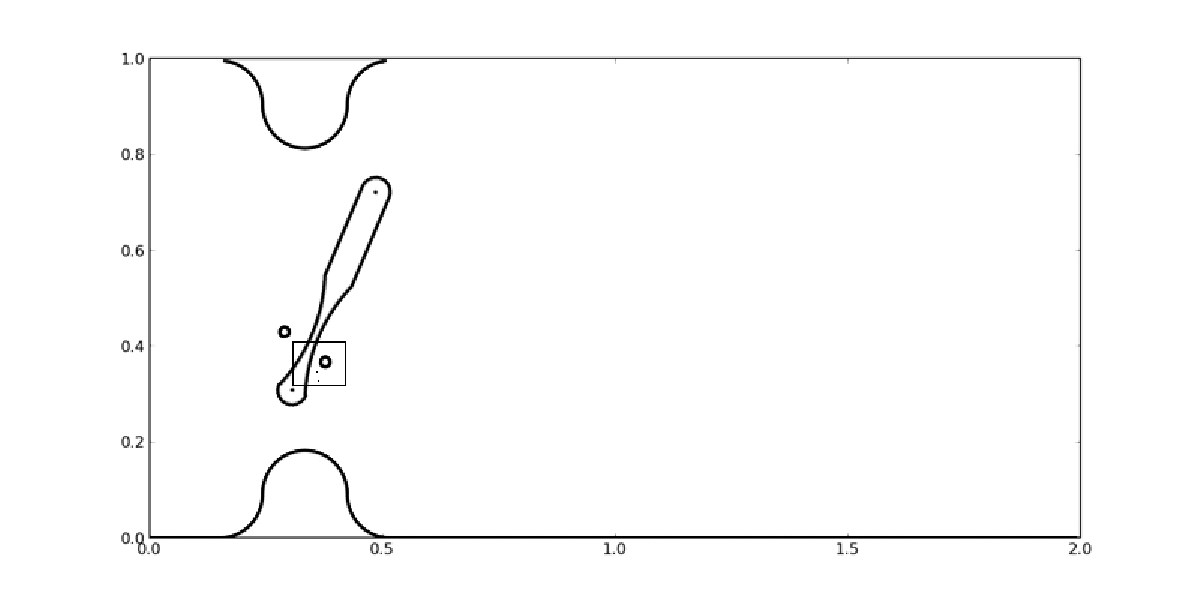
\includegraphics[bb=.5in .25in 7.35in 3.75in,width=5.25in,clip]{Images_Methodology/Box.pdf}
  \end{center}

  \caption{\small Configuration of our valve system after some period of time. The small box contains the subsystem of fiber points we solve exactly.}
  \label{fig:Box}
\end{figure}


\subsection{Numerical results}
The initial condition is a rest configuration of all links and tethers. The valve rests between the two hinges and is parallel to the $y$-axis. The imposed flow is $v_{flow}=100$ and all spring constants are taken to be $k=10^9l^{-2}$, where $l=h/2$ is the length between nodes in our valve. The magnitude of the velocities here reaches approximately 10 units,  much smaller than that in the elliptical membrane case. Taking a characteristic length to be the length of the heart valve we obtain a Reynolds number of about $5$. The smaller speeds lead to a mild CFL constraint and this allows our  semi-implicit approach to show its power, even though now $N_B \approx 4N$ and the cost of an implicit time-step is roughly $20$ times that of an explicit one.

For the FE/BE simulation $\Delta t$ is again taken to be the maximum allowable while retaining stability, with $\Delta t = 30h k^{-1/2}$. For the proposed semi-implicit approach we fix $\Delta t=0.0025$, well below the CFL restraint. 
With the
constant imposed flow, the valve will simply open. The CPU times for the explicit simulations are given in Table~\ref{table:ValveFEBESims} with the results from the implicit simulations following in 
Table~\ref{table:ValveImplicitSims}. With a less restrictive CFL constraint the semi-implicit approach becomes $O(1000)$
faster than FE/BE. Stability-wise,  $\Delta t$ may be taken even larger for the semi-implicit method,  up to the limit of the CFL restraint, leading to even greater savings in CPU time. However, this will typically increase leakage through the immersed boundary and eventually allow the valve to collide and pass through the hinges.

To open and close the valve we consider a time dependent imposed flow $v_{flow}(t)$.
We define
\begin{equation}
v_{flow}(t) =
\left\{
\begin{array}{cccc}
&60000t(0.1-t)& &t<0.1 \\
&-60000(t-0.1)(0.2-t)& &t\geq 0.1
\end{array}
\right. .
\label{eqn:VariableFlow}
\end{equation}
A sequence of snap-shots of the motion of the valve as it opens and closes is depicted in Fig.~\ref{fig:TimeProgression}
where also flooded contours of the vorticity are shown. Initially, there is a noticeable generation of (positive) vorticity at the upper and lower tips of the valve as the valve opens as well as in the upper cushion. As the valve reverses its motion the vorticity in those same
areas evolves toward positive values and becomes large and localized as the valve closes. 
 


\begin{table}
\caption{The number of Lagrangian nodes $N_B$ and the maximum stable timestep $\Delta t$ for a FE/BE method are given for increasing values of $N$.}
\label{table:ValveSimData}
\begin{center}
\begin{tabular}{|c|c c|}
\hline
$N$ & $N_B$ & $\Delta t$ \\
\hline
128 & 520 & $1.15\cdot 10^{-7}$ \\
256 & 1053 & $2.89\cdot 10^{-8}$ \\
384 & 1592 & $1.29\cdot 10^{-8}$ \\
512 & 2122 & $7.24\cdot 10^{-9}$ \\
\hline
\end{tabular}
\end{center}

\caption{Heart valve simulation with Forward Euler/Backward Euler scheme. The total CPU time taken to run the simulation up to time $T$ is given, with the average CPU time per timestep given. $^*$ denotes an extrapolated value.}
\label{table:ValveFEBESims}
\begin{center}
\begin{tabular}{|c|c c c c c|}
\hline
$N$ & Average & $T=0.01$ & $T=0.05$ &$T=0.1$ &$T=0.5$\\
\hline
128 & 0.024 & 2110.49 & 10508.95 & $21017.90^*$ & $105089.54^*$ \\
256 & 0.109 & $37687.16^*$ & $188435.83^*$ & $376871.66^*$ & $1884358.32^*$ \\
384 & 0.249 & $193168.57^*$ & $965842.85^*$ & $1931685.70^*$ & $9658428.53^*$ \\
512 &0.503 & $694291.69^*$ & $3471458.49^*$ & $6942916.98^*$ & $34714584.93^*$\\
\hline
\end{tabular}
\end{center}

\caption{Heart valve simulation with implicit scheme. The total CPU time taken to run the simulation up to time $T$ is given, with the average CPU time per timestep given. $\Delta t = 0.0025$.}
\label{table:ValveImplicitSims}
\begin{center}
\begin{tabular}{|c|c c c c c|}
\hline
$N$ & Average & $T=0.01$ & $T=0.05$ &$T=0.1$ &$T=0.5$\\
\hline
128 & 0.588 & 2.001 & 10.436 & 21.155 & 117.767\\
256 & 2.014 & 7.640  & 38.171 & 76.297 & 402.749\\
384 & 4.747 & 18.735 & 93.266 & 186.270 & 949.409\\
512 & 9.538 & 34.984 & 174.702 & 348.531 & 1907.635\\
\hline
\end{tabular}
\end{center}
\end{table}

\begin{figure}[p]
\begin{center}
%\includegraphics[bb=1.3in .5in 13.5in 6in,width=4.2in,clip]{Images_Methodology/fig_c10_n512.pdf}
%\hfill
\includegraphics[bb=1.3in .5in 13.5in 6in,width=4.2in,clip]{Images_Methodology/fig_c25_n512.pdf}
\hfill
\includegraphics[bb=1.3in .5in 13.5in 6in,width=4.2in,clip]{Images_Methodology/fig_c45_n512.pdf}
\hfill
\includegraphics[bb=1.3in .5in 13.5in 6.3in,width=4.2in,clip]{Images_Methodology/fig_c70_n512.pdf}
\hfill
\includegraphics[bb=1.3in .5in 13.5in 6.5in,width=4.2in,clip]{Images_Methodology/fig_c80_n512.pdf}
\end{center}
\caption{\small Vorticity field of our valve system through time. $N=512,N_B=2082,\Delta t=0.0025$. Frames shown at total simulation time $T=0.0625,0.1125,0.1750,0.2000$}
\label{fig:TimeProgression}
\end{figure}



\chapter{Peristaltic pumping, an application}
\noindent
We turn now to a fully featured application of the developed implicit methodology: peristalsis of a viscoelastic fluid.
Peristaltic pumping is a mechanism for transporting fluid prevalently utilized in both biological organisms and human designed systems. The mechanism induces flow in a channel by contracting the channel's walls in a set pattern. Peristaltic pumping of Newtonian fluids is well understood, and recent investigations have begun exploring the nature of peristalsis of non-Newtonian fluids. Here we investigate the particular case of peristalsis of an Oldroyd- B fluid via an Immersed Boundary method. Previous studies have investigated this same model, but have been hampered by stiffness constraints. Our intent here is to more fully explore the entire parameter regime pertaining to the model, including regimes where the polymeric stress is many orders of magnitude larger than previously accessible to numerical experiments. In particular,  we consider large Weissenberg numbers and high channel occlusions. A new dynamic behavior is observed with substantial effects on the pumping flow rate, including evidence for a finite-time blow up of the Oldroyd- B equations.

\graphicspath{./Images/}

\graphicspath{./Images/ResolutionStudy/}
\graphicspath{./Images/FullJaffrin/}
\graphicspath{./Images/Chi.8_Study/}

\graphicspath{./Images/Chi.8/_2000/}
\graphicspath{./Images/Chi.8/_6000/}
\graphicspath{./Images/Chi.8/_18000/}
\graphicspath{./Images/Chi.8_N512/_3000/}
\graphicspath{./Images/Chi.8_Newtonian/_3000/}

\graphicspath{./Images/W55/_2800/}
\graphicspath{./Images/W55/_16800/}
\graphicspath{./Images/W55/_37800/}


\section{Introduction}
Peristalsis is the predominant mechanism of action in a plethora of biological phenomena, from earthworm mobility to gastrointestinal and esophageal transport. Peristalsis is utilized in many mechanical fluid pumps, often because of their ability to effectively transport highly viscous fluids. In both biological and mechanical systems,  the fluid internal to the pump may be non-Newtonian. Such is the case for peristalsis in the oviduct and uterus where the transported biological fluid is highly complex.

Recent work has begun the investigation of peristalsis of an Oldroyd B (OB) fluid~\cite{teran2008peristaltic, chrispell2010peristaltic}. 
A marked difference has been reported with respect to the Newtonian flow counterpart, particularly the non-linear relationship between mean flow through the pump and the Weissenberg number of the fluid. It has been noted in these works that the polymeric stress of the transported fluid can lead to very strong normal stresses at the interface with the pump. These stresses present a difficult numerical problem. In order to correctly model the structure of the pump wall very stiff forces must be employed, leading to very small time-step constraints. Such numerical constraints (stiffness) are particularly pernicious for explicit Immersed Boundary (IB) methods, as used in~\cite{teran2008peristaltic, chrispell2010peristaltic}. There,  the numerical stiffness  limited the range of parameters ameanable to investigate. In Section~\ref{Sec:Methodology},  we present a new numerical method coupling a viscoelastic fluid solver to a novel, highly efficient semi-implicit implementation of the IB method, presented in more detail in~\cite{IBM_Implicit2D, IBM_Implicit3D}. The implicit methodology allows us to explore extreme parameter regimes previously out of reach of numerical algorithms. In particular, when the waves of peristalsis have very large amplitude, nearly occluding the channel, the normal stresses on the wall become extremely large. In addition, for very large Weissenberg numbers the transported fluid can develop very strong stresses, even for moderate occlusions. The implicit methodology allows us to robustly probe both of these regimes. Previous work has hinted at interesting behavior as the pump occlusion is increased, including substantial effects on the pump's rate of flow. We probe these effects  for substantially larger occlusions than previously possible. In Section~\ref{sec:Results} we detail new behavior observed, including evidence for a finite-time blow up of the OB equations.




\section{The Peristaltic Pump and Viscoelastic Fluid Models}
\label{Sec:Models}
We consider a peristaltic pump immersed in a period 2D domain $\Omega=[0,1]^2$.
We model the peristaltic pump as two disconnected sinusoidal curves,
\begin{equation}
\B{X}(t) =
\label{eq:Pump2D}
\left\{
\left(\xi, \frac{1}{2} + d(\xi,t)\right) \Big{|} \xi\in[0,1]
\right\}
\cup
\left\{
\left(\xi, \frac{1}{2} - d(\xi,t)\right) \Big{|} \xi\in[0,1]
\right\}
\end{equation}
where
\begin{equation}
\label{eq:d}
d(x,t) = \frac{\alpha}{2\pi}[1 + \chi \sin 2\pi(\xi - t)].\\
\end{equation}
Both the spatial and temporal period of the pump is fixed at $1$. As time progresses the waves of peristalsis move from left to right, forcing the fluid to flow to the right (in aggregate). The parameter $\chi$ represents the occlusion ratio of the pump. The value $\chi=0$ corresponds to a straight channel , with no waves of peristalsis, while $\chi=1$ correspond to a completely occluded channel, with the peaks of each sinusoidal curve meeting at some point along the horizontal line $y=1/2$. The parameter 
$\alpha$ controls  the aspect ratio of the channel. For this work we fix $\alpha=1.5$.

We model the interior and exterior of the valve as one continuous Oldroyd B (OB) incompressible fluid. The interaction between the valve and the fluid is captured via the Immersed Boundary Method. The continuous equations are then
\begin{align}
Re \left(\frac{\partial \B{u}}{\partial t} + \B{u}\cdot\nabla\B{u} \right) &= -\nabla p +  \nabla^2 \B{u} + \beta\nabla\cdot\B{S} + \B{f}, \label{eq:OB_momentum}\\ 
\nabla \cdot \B{u} &= 0, \label{eq:OB_incompressibility}\\
\frac{\partial \B{X}}{\partial t}  &= \B{u}(\B{X},t), \label{eq:OB_noslip}\\
\B{S}^\nabla &= -{We}^{-1}(\B{S} - \B{I}). \label{eq:OB_stress}
\end{align}
Here $\B{f}$ can be seen as a Lagrange multiplier used to enforce the prescribed motion of the peristaltic waves. Due to the no slip boundary condition (\ref{eq:OB_noslip}) we can only modulate $\B{X}$ by modifying the fluid velocity $\B{u}$. In practice,  we will only enforce the prescribed position of $\B{X}$ approximately by taking $\B{f}$ to be  a very stiff force binding the current configuration $\B{X}$ to the desired prescribed position given by (\ref{eq:Pump2D}).

In (\ref{eq:OB_momentum}), $Re$ is the Reynolds number which is a measure of the viscous dissipation relative to inertial forces. The dimensionless term $\beta$  specifies the strength of the viscoelastic force $\nabla\cdot\B{S}$. Here, $\B{S}$ is the deviatoric part of of the viscoelastic stress tensor and evolves according to the OB constitutive equation, given in (\ref{eq:OB_stress}). $\B{S}^\nabla$ denotes the upper convected derivative of $\B{S}$, namely
\begin{equation}
\B{S}^\nabla = \frac{d\B{S}}{dt} + \B{u}\cdot\nabla\B{S} - \nabla \B{u} \cdot \B{S} - \B{S} \cdot \nabla\B{u}^T.
\end{equation}
 $We$ is a dimensionless parameter giving the ratio of the relaxation time of the polymeric stress $\B{S}$ against some characteristic time scale of the fluid. $We$ is referred to as the Weissenberg number of the fluid. In the limit as $We\to 0$ the polymeric stress is fixed as the identity tensor $\B{I}$ and the fluid becomes Newtonian. In general the larger the value of $We$ the larger the non-Newtonian effect on the fluid.

Finally, the product $\beta We$ is the ratio of the polymeric viscosity to the solvent viscosity. Following Teran, Fauci, Shelly~\cite{teran2008peristaltic}
we fix $\beta We=\frac{1}{2}$. As mentioned above, we choose the characteristic length scale to be $1$, the width of our fluid domain $\Omega$ and the characteristic timescale we also take it  to be $1$, the period of the peristaltic pump. We fix the Reynolds number of our fluid at $Re=1$. Throughout this work the only fluid parameter we change is the Weissenberg number $We$.





\section{Methodology}
\label{Sec:Methodology}
We discretize the peristaltic pump $\B{X}$ as a collection of $N_B$ immersed points $\left\{\B{X}_j\right\}$. The position of these points are not directly prescribed, rather we construct an artificial force to approximately constrain the immersed points to their respective positions. For each point $\B{X}_j$ we define $\B{T}_j$ to be the desired target position. We then induce a force $\B{F}$ defined on immersed points given by
\begin{equation}
\B{F} = \sigma(\B{T} - \B{X}).
\label{eq:Force}
\end{equation}
The scalar variable $\sigma$ is a numerical parameter. In the limit as $\sigma\to\Inf$ we exactly constrain $\B{X}$ to the desired configuration. In practice we take $\sigma$ to be some large value. This can lead to instability in the resulting numerical simulations. We counter this by employing a new semi-implicit methodology as detailed in~\cite{IBM_Implicit2D, IBM_Implicit3D}. With the semi-implicit method we can use values of $\sigma$ multiple orders of magnitude larger than previously possible. For the large values of $We$ and $\chi$ explored in this work we are required to take $\sigma=O(10^6)$ to maintain the structure of the pump. This large stiffness coefficient would lead to prohibitively small time-steps for previous explicit methods. In our numerical experiments our choice of $\sigma$ reduces deviations in $\B{X}$ from the target position $\B{T}$ to less than $.0005$ units, even when the normal polymeric stresses at the boundary rise to values of $1000$ and more.

We briefly overview the semi-implicit method here. The method is based on a semi-implicit discretization of the Navier-Stokes equations given by
\begin{align}
\frac{\B{u}^{n+1}-\B{u}^n}{\Delta t} + \B{u}^n\cdot\nabla\B{u}^n &= -\B{D}_h p^{n+1}+ L_h \B{u}^{n+1} + \B{f}, \label{eq:dmoment} \\
\B{D}_h \cdot \B{u}^{n+1} &= 0, \label{eq:ddivergence} \\
\frac{\B{X}^{n+1}-\B{X}^n}{\Delta t} &= \C{S}^*_n\B{u}^{n+1}. \label{eq:Xt}
\end{align}
Here a superscript $n$ denotes a numerical approximation taken at the time $n \Delta t$ and $\Delta t$ is the timestep. The spatial operators $\B{D}_h$ and $L_h$ are the standard,  second order approximations to the gradient and the Laplacian, respectively. The convection term $\B{u}^n\cdot\nabla\B{u}^n$ is handled separately via a third-order essentially non-oscillatory (ENO) scheme.
The force $\B{F}$ in (\ref{eq:Force}) is defined at the immersed points and can not be directly used in the fluid equations (\ref{eq:OB_momentum})-(\ref{eq:OB_stress}). First we must {\em spread} the force onto the surrounding Eulerian grid. Likewise in equation (\ref{eq:Xt}) the fluid velocity is not given at the immersed points, so we must {\em interpolate} the fluid velocity. To achieve the spreading and interpolation we define
\begin{align}
(\C{S}_n G) (\B{x})&= \sum_{s \in \C{G}_B }G(s) \delta_h(\B{x}-\B{X}^n(s))h_B,
\label{eq:S} \\
(\C{S}^*_n w)(s) &= \sum_{ \B{x} \in \C{G}_\Omega} w(\B{x})\delta_h(\B{x}-\B{X}^n(s))h^2,
\label{eq:S*}
\end{align}
known as the spreading and interpolation operators, respectively.
Here $\delta_h(\B{x}) \equiv d_h(\B{x}_0)d_h(\B{x}_1)$ is an approximation to the two-dimensional Dirac delta distribution and $d_h$ is given by
\begin{equation}
d_h(r) = \begin{cases}
\frac{1}{4h}\left( 1+\cos(\frac{\pi r}{2h})\right)& \textrm{if } |r|\leq 2h, \\
0& \textrm{otherwise}.
\end{cases}
\end{equation}
We refer to these operators as lagged because the interface configuration $\B{X}^n$ is used 
instead of the future configuration $\B{X}^{n+1}$.

Utilizing $\C{S}_n$ and $\C{S}^*_n$ we now specify the form of $\B{f}$ in (\ref{eq:dmoment}).
\begin{equation}
\B{f} = \sigma\C{S}_n(\B{T}^{n+1} - \B{X}^{n+1}) + \beta\B{D}_h\cdot\B{S}^n,
\end{equation}
encapsulating both the artificial force on the immersed points, as well as the additional force coming from the polymeric stress. We thus consider the polymeric stress fixed as we update the fluid. Once we have an updated fluid velocity $\B{U}^{n+1}$ we will then calculate an updated value for the stress $\B{S}^{n+1}$.

We may formally eliminate $\B{u}^{n+1}$ from the equations (\ref{eq:OB_momentum})-(\ref{eq:OB_stress}), arriving at a {\em linear} system of the form
\begin{equation}
\B{X}^{n+1} = \sigma\C{M}_n(\B{T}^{n+1} - \B{X}^{n+1}) + \B{b}^n, \label{eq:LagrangianSystem}.
\end{equation}
We refer to this as the Lagrangian system. $\C{M}_n$ is an operator acting on a force distribution $\B{F}$ and returning the resulting displacement of immersed points due to the induced fluid flow from the spread force $\C{S}_n\B{F}$. Critically, both $\C{M}_n$ and $\B{b}^n$ can be explicitly constructed in an efficient manner, yielding a $2N_B\times 2N_B$ matrix and $2N_B$ vector respectively. We detail this construction in our previous papers~\cite{IBM_Implicit2D, IBM_Implicit3D}. The resulting system can be rewritten as a simple matrix inversion problem
\begin{equation}
(I + \sigma\C{M}_n)\B{X}^{n+1} = \sigma \B{T}^{n+1} + \B{b}^n, \label{eq:MatrixProblem}.
\end{equation}
The matrix $I + \sigma\C{M}_n$ is positive-definite and the system (\ref{eq:MatrixProblem}) can be inverted in a number of ways, the most efficient being multigrid. For the present work conjugate gradient suffices to provide a nearly optimal solver. Once we have solved (\ref{eq:MatrixProblem}) for the updated configuration $\B{X}^{n+1}$ we may then calculate the updated fluid velocity via (\ref{eq:OB_momentum})-(\ref{eq:ddivergence}).

\Comment{
We note that other work done investigating the peristaltic pump via the Immersed Boundary Method has utilized staggered marker and cell (MAC) grids. While our implicit methodology easily extends to MAC grids, we instead employ a simple Eulerian grid so as to utilize a Fast Fourier Transform (FFT) based fluid solver to solve (\ref{eq:dmoment})-(\ref{eq:ddivergence}). There may be advantages to a MAC grid, however, such as better volume conservation~\cite{griffithvolume}.
}

Finally we must calculate the updated polymeric stress $\B{S}^{n+1}$. Recall the constitutive equation (\ref{eq:OB_stress}) given as $\B{S}^\nabla = -{We}^{-1}(\B{S} - \B{I})$. We discretize this in space as
\begin{equation}
\frac{d\B{S}}{dt} + \B{u}^{n+1}\cdot\nabla\B{S}^n
 = \B{D}_h \B{u}^{n+1} \cdot \B{S}^n + \B{S}^n \cdot \B{D}_h(\B{u}^{n+1})^T + \frac{1}{We}(\B{I} - \B{S}^n).
\end{equation}
Here the convective term $\B{u}^{n+1}\cdot\nabla\B{S}^n$ is calculated via the third-order ENO scheme, as with the convection in the momentum equation (\ref{eq:dmoment}). We further discretize in time via a second-order total variation diminishing (TVD) Runge-Kutta method. If we define the Euler update operator
\begin{equation}
E(\B{S}) = \B{S} + \Delta t \left[\B{D}_h \B{u}^{n+1} \cdot \B{S} + \B{S} \cdot \B{D}_h(\B{u}^{n+1})^T + \frac{1}{We}(\B{I} - \B{S}) - \B{u}^{n+1}\cdot\nabla\B{S}\right],
\end{equation}
then our Runge-Kutta update is given as $\B{S}^{n+1} = (\B{S}^n + E(E(\B{S}^n))) / 2$.

\subsection{Summary of algorithm}
Given $\B{X}^n$, $\B{u}^n$, $\B{S}^n$ at time $t=n\Delta t$, a complete timestep may be summarized as follows
\begin{enumerate}
\item Calculate the fluid matrix $\C{M}_n$ and the explicit term $\B{b}^n$.
\item Solve for the updated pump configuration $\B{X}^{n+1}$ via the matrix problem $(I + \sigma\C{M}_n)\B{X}^{n+1} = \sigma \B{T}^{n+1} + \B{b}^n$.
\item Calculate the updated fluid velocity $\B{u}^{n+1}$ via the Stokes problem (\ref{eq:dmoment})-(\ref{eq:ddivergence}).
\item Calculate the updated polymeric stress $\B{S}^{n+1}$ via the second-order TVD Runge-Kutta method, $\B{S}^{n+1} = (\B{S}^n + E(E(\B{S}^n))) / 2$.
\end{enumerate}



\section{Results}
\label{sec:Results}
Here we summarize the results of our numerical simulations. We first present evidence to validate our methodology and then proceed to explore the extreme parameter regimes corresponding to very large wave amplitudes (occlusions) and very large Weissenberg numbers. We observe a new rich behavior which includes the potential formation of a finite time blow-up in the Oldroyd B model.

Two important values we will be observing are the flux and the normalized mean flow. We define the flux as
\begin{equation}
\label{eq:Flux}
Q(x,t) = \int^{0.5+d(x,t)}_{0.5-d(x,t)}u(x,y)dy,
\end{equation}
which is the total mass flux within the peristaltic pump across a specified vertical line. In this work we always take $x=0.5$ and write $Q(t)=Q(x,t)$ for convenience. Closely related to the flux is the normalized mean flow, given by
\Comment{
\begin{equation}
\label{eq:MeanFlow}
\Theta = \frac{\pi}{\alpha\chi(T_2-T_1)}
\int^{T_2}_{T_1} Q(t) dy dt.
\end{equation}
Here we simply average and normalize the flux over the time period $[T_1,T_2]$.}
\begin{equation}
\label{eq:MeanFlow}
\Theta(t) = \frac{\pi}{\alpha\chi}
\int^{t+1}_{t} Q(t) dt.
\end{equation}
Here we simply average and normalize the flux over one period of the peristaltic pump. The normalization leads to a dimensionless value, and is chosen such that $\Theta=1$ when $\chi=1$, regardless of the nature of the underlying fluid.

\Comment{
\begin{equation}
\label{eq:MeanFlowExpanded}
\Theta = \frac{\pi}{\alpha\chi(T_2-T_1)}
\int^{T_2}_{T_1} 
\int^{0.5+d(x,t)}_{0.5-d(x,t)}u(x,y)dy
 dt
\end{equation}
}


\subsection{Resolution study and comparison to analytical results}
We seek to validate our simulations through two approaches, by performing a spatial resolution study as well as by comparing simulations to known analytical results.

For the resolution study we consider the case when $\chi=0.25$ and $We=1$. We fix the time-step $\Delta t=0.00025$ and run the simulation for a range of $N$ from $N=256$ up to $N=2048$. We consider the $N=2048$ run as our reference solution ("exact")
and compute the errors of the other simulations in relation to this $N=2048$ case. The results are given in Figure~\ref{fig:ResolutionStudy}. In Figure~\ref{fig:ResolutionStudy_flow} we examine the difference in flow $Q$ at time $t=1$. We observe less than a $1\%$ relative error in $Q$ for $N \geq 1024$. In Figure~\ref{fig:ResolutionStudy_supS} we consider the sup norm of the difference of the $xx$-component of the stress. In both cases we observe slightly better than first order convergence, as expected from the convergence of the IB method. 

There is a known analytic approximation of the mean flow $\Theta$ for the case of a Newtonian Stokes flow ($Re=0$ and $We=0$) due to Jaffrin and Shapiro~\cite{jaffrin1971peristaltic}. The formula is given as
\begin{equation}
\label{eq:Jaffrin}
\Theta_J = \frac
{15\chi^2 + 2\alpha^2[4(1-\chi^2)^{5/2} + (7\chi^2-4)(1-\chi^2)]}
{\chi[5(2+\chi^2) + 6\alpha^2\chi^2(1-\chi^2)]}
\end{equation}
In the Newtonian Stokes case $\Theta$ is a constant, thus the time of evaluation is not important so long as $T\geq 1$. In contrast our Navier-Stokes fluid has convection and takes a finite amount of time ($t < 1$) to reach a steady state. We take $t=1$ and calculate $\Theta$ for a full range of $\chi$, from $0$ up to $0.95$. We note that as $\chi\to 1$ the normal stresses on the walls of the pump become enormous. While the value $\sigma=10^6$ is sufficient for $\chi=0.95$, we note that for the case $\chi=1$ even the extremely large value $\sigma=10^8$ is insufficient to maintain the shape of the pump. In this extreme case the implicit methodology remains stable but the distortion of the geometry is great enough to warrant omitting the calculated mean flow.

The comparison of our simulated results, which have been checked under time and space refinement,  to Jaffrin and Shapiro's formula can be seen in Figure~\ref{fig:Jaffrin}. We see reasonably good agreement. We note, however, that for small to moderate occlusion ratios,  the Stokes-OB results in~\cite{teran2008peristaltic}  and our own results from explicit simulations provide slightly better agreement with the analytic formula. From our experience,  we tend to believe that this small difference might be attributed to the somewhat better volume conservation of the explicit method. Importantly, however, explicit simulations for the cases when $\chi>0.5$ become impractical. 


% Resolution study
\Comment{
\begin{figure}[p]
\begin{center}
\doublefigure{ResolutionStudy/ResolutionStudy_flow_vs_N_log.png}
\doublefigure{ResolutionStudy/ResolutionStudy_supS_vs_N_log.png}
\end{center}
\caption{\small .}
\label{fig:ResolutionStudy}
\end{figure}
}

\begin{figure}
    \centering
    \subfigure[Error of normalized flow $|Q - \tilde{Q}|$, $m=-1.479$.]
    {
			\singlefigure{ResolutionStudy/ResolutionStudy_flow_vs_N_log.png}
			\label{fig:ResolutionStudy_flow}
    }
    \subfigure[Error of maximum stress $\norm{S_{xx} - \tilde{S}_{xx}}_\Inf$, $m=-1.800$.]
    {
			\singlefigure{ResolutionStudy/ResolutionStudy_supS_vs_N_log.png}
			\label{fig:ResolutionStudy_supS}
    }
    \caption{Spatial resolution study for decreasing values of $h$. Value specified is plotted against $h$ in a log-log plot. Variables with a tilde, $\tilde{\Box}$, refer to values coming from an $N=2048$ simulation taken to be an exact solution. Dashed lines are linear fits with specified slope $m$.}
    \label{fig:ResolutionStudy}
\end{figure}

% Jaffrin's curve and comparison
\singlefigureall{FullJaffrin/Jaffrin.png}{Normalized mean flow calculated both via Jaffrin and Shapiro's formula and numerical simulation for the full range of $\chi=0$ to $\chi=1$.}{Jaffrin}


\subsection{High occlusion, $\chi$=.8}
Previous investigations utilizing the IB method to study peristaltic pumping have been limited to occlusions $\chi \leq 0.5$. With
our implicit methodology we are able to explore for the first time occlusions in the range $0.5 < \chi <1$ which induce extremely large polymeric stress forces  on the peristaltic pump. Here we focus specifically on the case $\chi=0.8$ and $We=5$.

In Figures~\ref{fig:TimeProgression_Chi.8_xx} through~\ref{fig:TimeProgression_Chi.8_vorticity} we plot the polymeric stress evolution over time, for $N=1024$ and $\Delta t=0.00025$. We see first that the $xx$ component of stress develops a strong concentration at the channel's neck, reaching a value of $360$ at time $t=0.5$. Soon after, at time $t=1.5$, the $xx$-component is further concentrated into a nearly horizontal line, reaching a peak value of $18000$. The two additional components $\B{S}_{xy}$ and $\B{S}_{yy}$ develop strong interfaces in identical locations, reaching values of $2400$ and $6400$ respectively. These strong interfaces effectively block off the inner interior of the peristaltic pump from any outside influences. This can be clearly seen in the vorticity plot, where the vorticity inside the interfaces is nearly zero. Outside the interfaces, near the boundary of peristaltic pump, we see strong, nearly uniform vorticity. As time progresses further, up to $t=4.5$, we see the formation of more complex localized structures which again have strong effects on the vorticity. These fine structures eventually leads to instabilities and we are unable to reliably compute for longer than $t=7$ for $N\geq 512$.

An important observation is that the strong thin line observed in the $xx$-component of the stress at time $t=1.5$ dissipates over time and is significantly weaker at time $t=4.5$. We suspect that this dissipation is due to numerical diffusion inherent to the ENO advection scheme. To investigate this further we perform a resolution study, focusing on the peak value of $\B{S}_{xx}$ over the time interval $t=0$ to $t=1.5$.

First, in Figure~\ref{fig:Chi8Study_supmid} we plot $\B{S}_{xx}$ over time for values of $N$ ranging from $N=256$ to $N=2048$. We see that there is fast, nearly exponential growth, that levels off near $t=1.5$. As $N$ increases the maximum stress increases as well. We analyze the dependence on $N$ in Figure~\ref{fig:Chi8Study_log}. Here we plot $\norm{\B{S}_{xx}}_{\Inf}$ at $t=1.25$ versus $\log N$. We see that $\norm{\B{S}_{xx}}_{\Inf}$ grows almost exactly proportional to $\log N$, yielding the approximate formula
%$\norm{\B{S}_{xx}}_{\Inf} \approx 5286\log N$.
\begin{equation}
\norm{\B{S}_{xx}}_{\Inf} \approx 5286\log N.
\label{eq:ApproxGrowth}
\end{equation}
It is unclear if the relationship (\ref{eq:ApproxGrowth}) persists for arbitrarily large $N$. If this were the case then it would be evidence for a finite time blow up in the Oldroyd-B model for peristaltic pumping. To provide additional evidence we attempt to fit an exponential growth model of the form $C_Ne^{\beta_N t}$ to the stress $\norm{\B{S}_{xx}}_{\Inf}$ over the time interval $(0.36,0.70)$. For $N=2048$ the best fit is given by $C=10, \beta=7.68$. The fit is qualitatively good, as seen in Figure~\ref{fig:Chi8Study_GrowthFit_Exponential}. We proceed to compute the best fit for various values of $N$ and investigate the sequence $\{\beta_N\}$. In Figure~\ref{fig:Chi8Study_GrowthFitVsN_C_beta} we plot $\beta_N$ with respect to $\log N$ and notice a distinct linear trend. A linear fit yields $\beta_N\approx 0.3533\log N$. We thus again see sharper growth as $N\to\Inf$. This apparently unbounded behavior for the exponent points in the direction of a potential finite-time singularity in the polymeric stress. 

The simulation for $\chi=0.8$ is very challenging, involving very large stress and equally large restorative forces from the immersed structure. Very sharp interfaces develop in both the vorticity and stress. We present evidence that we are properly resolving these sharp interfaces. In Figure~\ref{fig:Chi8Compare} we plot a simulation at time $t=1.5$ for the case $\chi=0.8, We=5$. We compare the vorticity fields for both $N=512$ and $N=1024$ and note that the structure is qualitatively identical. Closer examination of the $N=512$ plot reveals slightly blurred interfaces, indicative of the greater numerical diffusion at lower resolutions. We observe similar results when we investigate the stress $\B{S}$. We look at the Newtonian case in Figure~\ref{fig:Chi8Compare_Newtonian} and note that the vorticity is well resolved. Indeed, we have observed that for the Newtonian case the vorticity is well resolved even for substantially lower resolutions, down to $N=256$. The difference between the vorticity distributions of Newtonian and viscoelastic cases is striking. 
\input

\clearpage

\begin{figure}
\doublefigure{Chi.8_N512/_3000/_vorticity.png}{Chi.8/_6000/_vorticity.png}
\caption{A comparison of the vorticity for a valve with $\chi=.8$ and $We=5$  at time $t=1.5$ for $N=512$ and $N=1024$ on the left and right respectively.}
\label{fig:Chi8Compare}
\end{figure}

\singlefigureall
{Chi.8_Newtonian/_3000/_vorticity.png}
{Vorticity for a valve with occlusion $\chi=.8$ in a Newtonian flow at time $t=1.5$.}
{Chi8Compare_Newtonian}


\Comment{
\begin{figure}
    \centering
    \subfigure[$N=1024, We=5$]
    {
			\singlefigure{Chi.8/_6000/_vorticity.png}
			\label{fig:Chi8Compare_1024}
    }
    \subfigure[$N=512, We=5$]
    {
			\singlefigure{Chi.8_N512/_3000/_vorticity.png}
			\label{fig:Chi8Compare_512}
    }
    \subfigure[$N=1024$, Newtonian]
    {
			\singlefigure{Chi.8_Newtonian/_3000/_vorticity.png}
			\label{fig:Chi8Compare_Newtonian}
    }
    \caption{A comparison of the vorticity for a valve with occlusion $\chi=.8$ at time $t=1.5$. For $We=5$ we look at $N=512$ and $N=1024$. For the Newtonian case we look at $N=1024$.}
    \label{fig:Chi8Compare}
\end{figure}
}



\Comment{
We provide a simple linear analysis to suggest otherwise.

Suppose that the maximum value of $\B{S}_{xx}$ at time $t$ occurs at position $\B{x}(t)$, and that this location is fixed, save for convection due to the fluid. We note that for the time range we are considering this is indeed what we observe. Then, for very large $S\equiv\B{S}_{xx}(\B{x})$, the OB constitutive equation for $S$ should be approximated well by
\begin{equation}
\frac{dS}{dt} \approx \frac{\partial u}{\partial x}S + \frac{1}{We}[1-S],
\end{equation}
where we have dropped the convection term since $\B{x}$ is convected with the fluid, and we have dropped the $\partial u / \partial y$ term because it is zero along the horizontal line $y=0.5$ due to symmetry. We empirically observe that $\partial u / \partial x \gg 1/We$, and, furthermore, that $\partial u / \partial x$ remains relatively close to some constant $C$. Thus for large $S$ we have that $dS/dt \approx CS$ yielding simple exponential growth. While this growth would not lead to finite time blow ups, it does not appear that any term in the constitutive equation (\ref{eq:OB_stress}) can ever balance the growth of $S$, thus we still expect $S\to\Inf$ as $t\to\Inf$, an unphysical result.
}


% \Chi = .8 study
\begin{figure}
    \centering
    \subfigure[$\norm{\bar{S}_{xx}(t)}_\Inf$ over the time interval $(0,1.5)$ for various values of $N$.]
    {
			\singlefigure{Chi.8_Study/Chi.8_supmid.png}
			\label{fig:Chi8Study_supmid}
    }
    \subfigure[$\norm{\bar{S}_{xx}(t)}_\Inf$ at time $t=1.25$, plotted against $-\log h$, as $N$ varies from $256$ to $2048$. Dashed line is a linear fit with slope $m=5286$]
    {
			\singlefigure{Chi.8_Study/Chi.8_T1.25_log.png}
			\label{fig:Chi8Study_log}
    }
    \caption{Resolution study of the sup norm of the stress component $S_{xx}$ along the horizontal line of symmetry, denoted as $\norm{\bar{S}_{xx}(t)}_\Inf$ at time $t$.}
    \label{fig:Chi8Study}
\end{figure}


\begin{figure}
    \centering
    \subfigure[$\norm{\bar{S}_{xx}(t)}_\Inf$ over the time interval $(0.36,0.70)$ for $N=2048$. Matched fit is the exponential curve $10e^{7.68t}$.]
    {
			\singlefigure{Chi.8_Study/Chi.8GrowthFit_Exponential.png}
			\label{fig:Chi8Study_GrowthFit_Exponential}
    }
    \subfigure[$\beta_N$ $(\circ)$ and $C_N$ $(\square)$ with respect to $\log N$. The solid line is a linear fit with slope $m=0.3533$]
    {
			\singlefigure{Chi.8_Study/Chi.8GrowthFitVsN_C_beta.png}
			\label{fig:Chi8Study_GrowthFitVsN_C_beta}
    }
    \caption{Consider $\norm{\bar{S}_{xx}(t)}_\Inf$ over the timer interval $(0.36,0.70)$ for a specified resolution $N$. We compute a best fit of the form $C_Ne^{\beta_N t}$, in the $L^2$ sense.}
\end{figure}


\subsection{High Weissenberg number}
Large values of $We$ lead to large normal forces on the walls of the peristaltic pump. These forces in turn require large stiffness constants $\sigma$ to properly maintain the prescribed shape of the walls. Previous investigations by Teran, Fauci and Shelley~\cite{teran2008peristaltic} and Chrispell and Fauci~\cite{chrispell2010peristaltic} were limited to Weissenberg numbers $We\leq 5$. With our superior methodology we are able to investigate for the first time higher Weissenberg numbers, up to and beyond $We=100$.

We investigate first the case $We=55$, $\chi=0.5$.
In Figures~\ref{fig:TimeProgression_W55_xx} through~\ref{fig:TimeProgression_W55_vorticity} we plot the polymeric stress evolution over time, for $N=1024$ and $dt=.00025$. We note first that all components of the stress $\B{S}_{xx}, \B{S}_{xy}, \B{S}_{yy}$ develop multilayered interfaces by time $t=8.4$. As time progresses, however, these interfaces merge into smooth, simple regions. By time $t=18.9$ no indication is left of the intricate, multilayered interfaces. We suspect that this smoothing is due to the numerical diffusion inherent to the ENO convection scheme.

An interesting question is how the normalized mean flow $\Theta$ responds to changes in $We$ and $\chi$. In Figure~\ref{fig:FullJaffrin} we plot $\Theta$ at time $t=15$ (Figure~\ref{fig:FullJaffrin_15}) and $t=50$ (Figure~\ref{fig:FullJaffrin_50}) for $We=0$ up to $We=105$, and for $\chi=0$ up to $\chi=0.75$. We note a modest effect of the Weissenberg number on $\Theta$, with higher values of $We$ corresponding to higher mean flows. The dependence of $\Theta$ on $t$ is more complicated. For $We\leq 5$ it appears that a semi-steady state is eventually reached. The time required to reach this semi-steady state was given to be $3We$ in~\cite{teran2008peristaltic, chrispell2010peristaltic}. When we examine the same regimes as studied in ~\cite{teran2008peristaltic, chrispell2010peristaltic} ($\chi\leq 0.5$, $We\leq 5$), we see a similar requirement.

For higher $We$ we report substantially different behavior. We examine the mean flow over time in Figure~\ref{fig:FlowOverTime}. For $\chi=0.4$ and $We=5$, displayed in Figure~\ref{fig:FlowOverTime_Chi.4}, we see relatively little variation in mean flow over time, consistent with previous results. For $We\geq 25$, however, we see substantially more complex behavior. For $We=25$ the mean flow appears to become reasonably consistent after $t=70$, despite large variations. For $We=55$ and $We=105$ no semi-steady state is reached for our simulation times ($T<150$). For $\chi=0.6$ we see long term variation in the mean flow even for the small value of $We=5$. The flow appears to reach and maintain a semi-steady state for a long duration of time, from $t=20$ to $t=70$ ($50$ periods of the pump), but then has a sudden drop in mean flow at time $t=70$.

Examining the structure of the stress over time we see that there is symmetry breaking in the stress field at approximately the same time as the drop in mean flow. We observe a similar break in symmetry for the other long time scale simulations. Such an instability is noted as well in~\cite{thomases2009transition}. There symmetry breaking is noted for higher Weissenberg numbers $We\geq 5$, as we observe here. We suspect that it is this instability that is preventing a semi-steady behavior from emerging in the mean flow, and expect that the behavior will not become semi-steady even for greatly longer simulations.

% Full Jaffrin
\begin{figure}
    \centering
\Comment{ t = 8.5
    \subfigure[Normalized mean flow at time $t=8.5$ for various values of $We$ and $\chi$.]
    {
			\singlefigure{FullJaffrin/FullJaffrinVerbose_850.png}
			\label{fig:FullJaffrin_8.5}
    }
}
    \subfigure[Normalized mean flow at time $t=15$ for various values of $We$ and $\chi$.]
    {
			\singlefigure{FullJaffrin/FullJaffrinVerbose_1500.png}
			\label{fig:FullJaffrin_15}
    }
    \subfigure[Normalized mean flow at time $t=50$ for various values of $We$ and $\chi$.]
    {
			\singlefigure{FullJaffrin/FullJaffrinVerbose_5000.png}
			\label{fig:FullJaffrin_50}
    }
    \caption{Normalized mean flow at times $t=15$ and $t=50$ for various values of $We$ and $\chi$.}
    \label{fig:FullJaffrin}
\end{figure}

% Over time
\Comment{ Double figure
\begin{figure}[p]
\doublefigure{FullJaffrin/FullJaffrinOverTime_Chi0.4.png}{FullJaffrin/FullJaffrinOverTime_Chi0.6.png}
\caption{Mean flow $\Theta$ over time for various values of $We$. $\chi=0.4$ and $\chi=0.6$ on the left and right respectively.}
\label{fig:FlowOverTime_Chi.4.6}
\end{figure}
}

\Comment{ Stacked figures }
\begin{figure}
    \centering
    \subfigure[$\chi=0.4$]
    {
			\singlefigure{FullJaffrin/FullJaffrinOverTime_Chi0.4.png}
			\label{fig:FlowOverTime_Chi.4}
    }
    \subfigure[$\chi=0.6$]
    {
			\singlefigure{FullJaffrin/FullJaffrinOverTime_Chi0.6.png}
			\label{fig:FlowOverTime_Chi.6}
    }
\Comment{
    \subfigure[$\chi=0.7$]
    {
			\singlefigure{FullJaffrin/FullJaffrinOverTime_Chi0.7.png}
			\label{fig:FlowOverTime_Chi.7}
    }
}
    \caption{\small Mean flow $\Theta$ over time for various values of $We$. Top and bottom plot are for $\chi=0.4$ and $\chi=0.6$ respectively.}
    \label{fig:FlowOverTime}
\end{figure}



% Time progression for \Chi = .8
\clearpage

\newcommand{\threeplotchi}[1]{
\onethirdtopspace
\begin{center}
\onethirdfigure{Chi.8/_2000/#1}
\onethirdspace
\onethirdfigure{Chi.8/_6000/#1}
\onethirdspace
\onethirdfigure{Chi.8/_18000/#1}
\end{center}
\onethirdbottomspace
}

\newcommand{\tvalues}{$t=.5$, $t=1.5$, $t=4.5$}

\begin{figure}[p]
\threeplotchi{_xx.png}
\caption{\small $S_{xx}$ at times \tvalues.}
\label{fig:TimeProgression_Chi.8_xx}
\end{figure}

\begin{figure}[p]
\threeplotchi{_xy.png}
\caption{\small $S_{xy}$ at times \tvalues.}
\label{fig:TimeProgression_Chi.8_xy}
\end{figure}

\begin{figure}[p]
\threeplotchi{_yy.png}
\caption{\small $S_{yy}$ at times \tvalues.}
\label{fig:TimeProgression_Chi.8_yy}
\end{figure}

\begin{figure}[p]
\threeplotchi{_vorticity.png}
\caption{\small Vorticity of the fluid velocity at times \tvalues.}
\label{fig:TimeProgression_Chi.8_vorticity}
\end{figure}


% Time progression for W = 55
\clearpage

\newcommand{\threeplotW}[1]{
\onethirdtopspace
\begin{center}
\onethirdfigure{W55/_2800/#1}
\onethirdspace
\onethirdfigure{W55/_16800/#1}
\onethirdspace
\onethirdfigure{W55/_37800/#1}
\end{center}
\onethirdbottomspace
}

\renewcommand{\tvalues}{$t=1.4$, $t=8.4$, $t=18.9$}

\begin{figure}[p]
\threeplotW{_xx.png}
\caption{\small $S_{xx}$ at times \tvalues.}
\label{fig:TimeProgression_W55_xx}
\end{figure}

\begin{figure}[p]
\threeplotW{_xy.png}
\caption{\small $S_{xy}$ at times \tvalues.}
\label{fig:TimeProgression_W55_xy}
\end{figure}

\begin{figure}[p]
\threeplotW{_yy.png}
\caption{\small $S_{yy}$ at times \tvalues.}
\label{fig:TimeProgression_W55_yy}
\end{figure}

\begin{figure}[p]
\threeplotW{_vorticity.png}
\caption{\small Vorticity of the fluid velocity at times \tvalues.}
\label{fig:TimeProgression_W55_vorticity}
\end{figure}


\clearpage


\section{Conclusion}
\label{Sec:Conclusion}

Previous investigations into peristaltic pumping of OB fluids have revealed that the gross transport properties of the pump are highly sensitive to the underlying fluid parameters. Making use of a new implicit methodology we are able to explore a much broader parameter regime, observing new behavior both for high occlusion ratios and high Weissenberg numbers.

Future work will focus on extending this investigation to three dimensions, where preliminary results suggest new and different behavior. Importantly, in 3D we can investigate a plethora of novel asymmetrical pump geometries, including cork-screw like shapes. Preliminary results also suggest interesting differences when the OB fluid is replaced with a FENE-P fluid. Future work will explore these differences.




\chapter{Concluding Remarks}
\noindent
Implicit methods for alleviating the stiffness of the IB Method have been around for some time. Their implementation involves solving systems of equations typically thought to be prohibitively expensive. In this work we have explored new methods that allow for the efficient solution of the pertinent systems in a wide range of IB applications. In many cases we saw that the new methods allowed speedups of multiple orders of magnitude.

The approach used in this work was two fold. First, we developed new methods to accelerate computations of the form $\C{M}_n\B{F}$, either through a matrix method, shown in Chapter~\ref{part:Matrix} to be well suited for many 2D applications, or through a treecode method, shown in Chapter~\ref{part:Treecode} to be well suited for many 3D applications.

Second, we explored new iterative techniques for solving the linear system (\ref{meq:Xnl}). In Chapter~\ref{part:Matrix} we explored a multigrid approach, and in Chapter~\ref{part:Splitting} we explored the splitting method, suitable to cases where simple Krylov methods are inapplicable.

Ultimately, however, the specific form of $\C{A}_{h_B}$ can lead to an arbitrarily difficult system of equations to solve. In particular, if the Jacobian of $\C{A}_{h_B}$ is nondefinite and has eigenvalues of mixed magnitude, the iterative methods developed here will be ineffective. We are confident, however, that future work, by ourselves and others, will fill in such gaps in the methodology.
